\documentclass[a4paper]{article}
%AMDG
\usepackage{amsmath, amsthm, amssymb}
\usepackage{hyperref}
\usepackage[slovene]{babel}
\usepackage[utf8]{inputenc}
\usepackage[T1]{fontenc}
\usepackage{epigraph}
\usepackage{pdftexcmds}
\usepackage{fancyref, nameref}
\usepackage{epigraph}
\usepackage{cleveref}
\usepackage{verbatim}
\usepackage{enumitem}
\usepackage{multicol}
\usepackage[nomessages]{fp}
\usepackage{fancyhdr}
\usepackage{multirow}
\usepackage{mathtools}

\usepackage{tikz}


\parindent=0pt


% \epigraphsize{\small}% Default
\setlength\epigraphwidth{8cm}
\setlength\epigraphrule{0pt}

\usepackage{etoolbox}

\makeatletter
\patchcmd{\epigraph}{\@epitext{#1}}{\itshape\@epitext{#1}}{}{}
\makeatother


\newcounter{environment:definition_counter}

\newenvironment{definition}[1][\unskip]
{\vspace{0.5cm}\refstepcounter{environment:definition_counter}\textbf{Definicija \arabic{environment:definition_counter}: \textbf{#1}}}
{\bigskip}

\newcounter{environment:theorem_counter}

\newenvironment{theorem}[1][\unskip]
{\refstepcounter{environment:theorem_counter}\textbf{Izrek \arabic{environment:theorem_counter}:\textit{#1}}\itshape\\}
{\bigskip}

\newcounter{environment:statement_counter}

\newenvironment{statement}[1][\unskip]
{\refstepcounter{environment:statement_counter}\textbf{Trditev \arabic{environment:statement_counter}:\textit{#1}}}
{\bigskip}

\newcounter{example:example_counter}

\newenvironment{example}
{\textbf{Primer:}\\}
{\setcounter{example:example_counter}{0}}

\newenvironment{example_case}
{\refstepcounter{example:example_counter} \arabic{example:example_counter}.}
{\\}

\newenvironment{remark}
{\textbf{Opomba:}}
{}

\newenvironment{corollary}
{\underline{\textbf{Posledica:}}}
{}

%should rethink this
\newtheorem{lemma}{Lema}

\newcommand{\subscript}[2]{$#1 _ #2$}

\newcommand{\twopartdef}[4]
{
	\left\{
		\begin{array}{ll}
			#1 & \mbox{; } #2 \\
			#3 & \mbox{; } #4
		\end{array}
	\right.
}


\pagestyle{headings}
\pagestyle{fancy}
%\fancyhead[LE,RO]{\itshape \nouppercase \rightmark}
%\fancyhead[LO,RE]{\itshape \nouppercase Chapter \arabic{chapter}}


\lfoot{Skripta za Algebro 2}
\rfoot{Filip Koprivec}

%operatorji
\newcommand{\ord}{\ensuremath{\operatorname{red}}} % red grupe/elementa
\renewcommand{\ker}{\ensuremath{\operatorname{Ker}}} % red grupe/elementa
\newcommand{\Mod}[1]{ \ (\text{mod}\ #1)}



\begin{document}	
\title{Skripta za algebro 2}
\author{Filip Koprivec}

\date{\today}
\maketitle

\epigraph{“If I find in myself desires which nothing in this world can satisfy, the only logical explanation is that I was made for another world.”}{--- \textup{C. S. Lewis}}
\newpage

\tableofcontents

\newpage

\begin{comment}
Start of text
\end{comment}

\section{Osnovne algebrske strukture}
\subsection{Binarne operacije}
\begin{definition}[Binarna Operacija]
\label{def:binary_operation}
(tudi dvočlena operacija) $\circ$ na množici $\mathcal{S}$ je preslikava iz $\mathcal{S} \times \mathcal{S} \  v \ \mathcal{S}$.\\ Torej $\circ : \mathcal{S} \times \mathcal{S} \ \to \ \mathcal{S}$
\end{definition}

\begin{example}
Osnovna zgleda binarnih operacij na $\mathbb{Z}$ sta:

\begin{example_case}
Seštevanje: $(n,m) \mapsto n+m$
\end{example_case}
\begin{example_case}
Množenje: $(n,m) \mapsto n \times m$
\end{example_case}

\end{example}

Skalarni produkt v $\mathbb{R}^{2}$ \textbf{ni} binarna operacija.

Vektorski produkt v $\mathbb{R}^{3}$ \textbf{je} binarna operacija.
\\\\
\begin{definition}
\label{def:asociative_operation}
Operacija $\circ$ je \textbf{asociativna}, če ustreza enačbi
\begin{equation}
\label{eq:asociative_law}
\forall x,y,z \in \mathcal{S}.\ (x \circ y) \circ z = x \circ (y \circ z)
\end{equation}

\end{definition}

Enakost \ref{eq:asociative_law} imenujemo \textbf{Zakon o asociativnosti}\\
Operacije, ki jih bomo obravnavali bodo praviloma asociativne.

\begin{definition}
\label{def:comutative_operation}
Elementa $x,y \in \mathcal{S}$ \textbf{komutirata}, če velja 
\begin{equation}
x,y \in \mathcal{S}. x \circ y = y \circ x
\end{equation}
Če za poljubna dva elementa iz $\mathcal{S}$ velja
\begin{equation}
\label{eq:comutative_law}
\forall x,y \in \mathcal{S}. x \circ y = y \circ x
\end{equation}
pravimo, da je operacija $\circ$ komutativna.
Enakost \ref{eq:comutative_law} imenujemo \textbf{Zakon o komutativnosti}

\end{definition}
\begin{remark}
Kadar je iz konteksta razvidno, o kateri operaciji govorimo, pogosto namesto "$\circ$ je komutativna rečemo tudi $\mathcal{S}$ je komutativna"
\end{remark}

\begin{example}
\begin{example_case}
Operacija + na $\mathbb{Z}$ je tako asociativna in komutativna
\end{example_case}
\begin{example_case}
Operacija * na $\mathbb{Z}$ je tako asociativna in komutativna
\end{example_case}
\begin{example_case}
Operacija - na $\mathbb{Z}$ \textbf{ni} niti asociativna niti komutativna
\end{example_case}
\begin{remark}
Na operacijo odštevanja gledamo kot na izpeljano operacijo in ne kot na samostojna operacijo, saj jo vpeljemo preko seštevanja in pojma nasprotnega elementa.
\end{remark}

\begin{example_case}
Naj bo $\mathcal{X}$ poljubna neprazna množica. Z $F(\mathcal{X})$ označimo množico vseh preslikav iz $\mathcal{X}$ v $\mathcal{X}$. Naj bosta $f, g \in \mathcal{X}$, potem je $(f,g) \mapsto f \circ g$ (kompozitum funkcij) binarna operacija na $F(\mathcal{X})$.

\begin{remark}
Operacija je asociativna, in kadar $|\mathcal{X}| \geq 2$ ni komutativna
\end{remark}
\end{example_case}
\end{example}

\begin{definition}
\label{def:identity_element}
Naj bo $\circ$ binarna operacija na na $\mathcal{S}$ in $e \in \mathcal{S}$. $e$ se imenuje \textbf{nevtralni element}, če velja 
\begin{equation}
\label{eq:identity_element}
\forall x \in \mathcal{S}. e \circ x = x \circ e = x
\end{equation}

\end{definition}

\begin{example}
\begin{example_case}
$0$ je nevtralni element za seštevanje na $\mathbb{Z}$.
\end{example_case}
\begin{example_case}
$1$ je nevtralni element za množenje na $\mathbb{Z}$.
\end{example_case}
\begin{example_case}
$id_{x}$ (identična preslikava) je nevtralni element za $F(\mathcal{X})$
\end{example_case}
\end{example}

\begin{remark}
Nevtralni element nima zagotovljenega obstoja (recimo $+$ na $\mathbb{N}$ ali $*$ na sodih celih številih).
\end{remark}

\begin{statement}
\label{st:identity_unique}
Če nevtralni element obstaja, je en sam.
\begin{proof}
\label{pr:identity_unique}
Naj bosta $f,e \in \mathcal{S}$ nevtralna elementa.
$$e = e \circ f \text{\ \ // Ker je f nevtralni element}$$
$$e \circ f = f \text{\ \ // Ker je e nevtralni element}$$
$$e = f $$
\end{proof}
\end{statement}

\begin{definition}
\label{def:left_identity}
Element $e'$ je \textbf{levi nevtralni element}, če velja:
\begin{equation}
\label{eq:left_identity_element}
\forall x \in \mathcal{S}. e' \circ x = x
\end{equation}
\end{definition}

\begin{definition}
\label{def:right_identity}
Element $e''$ je \textbf{desni nevtralni element}, če velja:
\begin{equation}
\label{eq:right_identity_element}
\forall x \in \mathcal{S}. x \circ e'' = x
\end{equation}
\end{definition}

\begin{remark}
Levih in desnih nevtralnih elementov je lahko več

\begin{example}
\begin{example_case}
$\circ : (x,y) \mapsto y$.

Vsak element je levi nevtralni element
\end{example_case}
\begin{example_case}
$0$ je desni nevtralni element za odštevanje v $\mathbb{Z}$
\end{example_case}
\end{example}
\end{remark}

\begin{statement}
\label{st:identity_left_right_both}
Naj bo za operacijo $\circ$ $e'$ levi nevtralni element, $e''$ pa desni nevtralni element. Tedaj velja $e' = e'' = e$ (Sta si levi in desni nevtralni element enaka in je(sta) nevtralni element)
\begin{proof}
\label{pr:identity_left_right_both}
$$e' = e' \circ e'' = e''$$
\end{proof}
\end{statement}

\begin{definition}
\label{def:inner_operation}
Naj bo $\circ $ operacija na $\mathcal{S}$ in naj bo $\mathcal{T} \subseteq \mathcal{S}$. Rečemo, da je $\circ$ \textbf{notranja operacija na $\mathcal{T}$} ali da je množica \textbf{$\mathcal{T}$ zaprta za $\circ$ na $\mathcal{T}$} , če velja
\begin{equation}
\label{eq:inner_operation}
\forall t, t' \in \mathcal{T}. t \circ t' \in \mathcal{T}
\end{equation}

\end{definition}

\begin{example}
Množica $\mathbb{N}$ je zaprta za operaciji $+$ in $*$, ni pa zaprta za operacijo $-$.
\end{example}

\begin{definition}
\label{def:outer_operation}
Preslikavi iz $\mathcal{K} \times \mathcal{S}$ v $\mathcal{S}$ kjer $\mathcal{K} \neq \mathcal{S}$ rečemo \textbf{Zunanja binarna operacija}
\end{definition}

\begin{example}
\begin{example_case}
Množenje vektorja s skalarjem\\
$(\lambda, \vec{x}) \mapsto \lambda\vec{x}$, kjer je $(K = \mathbb{R}, S = \mathbb{R}^n)$\\
$\lambda (x_1, x_2, \dots , x_n) = (\lambda x_1, \lambda x_2, \dots ,\lambda x_n)$
\end{example_case}
\end{example}

\subsection{Polgrupe in monoidi}

\begin{definition}
\label{def:algebraic_structure}
\textbf{Algebrska struktura} je množica, opremljena z eno ali več operacijami (notranjimi ali zunanjimi), ki imajo določene lastnosti
\end{definition}

\begin{definition}
\label{def:semigroup}
\textbf{Polgrupa} je par množice $\mathcal{S}$ skupaj z \textbf{asociativno binarno operacijo}. Pišemo: $(\mathcal{S}, \circ)$
\end{definition}

\begin{remark}
Kadar je jasno o kateri operaciji govorimo, pogosto govorimo kar o polgrupi $\mathcal{S}$
\end{remark}

\begin{example}
\begin{example_case}
$(\mathbb{N}, +), \underbrace{(\mathbb{Z}, +), (\mathbb{Q}, +), (\mathbb{R}, +), (\mathbb{C}, +),\dots}_{Niso\ samo\ polgrupe\ ampak\ kar\ grupe}$
\end{example_case}
\end{example}
\\
\\
Naj bo $(\mathcal{S}, \circ)$ polgrupa, po zakonu \ref{eq:asociative_law} o asociativnosti velja:
$$\forall x,y,z \in \mathcal{S}.\ (x \circ y) \circ z = x \circ (y \circ z)$$zato lahko oklepaje spuščamo in vse to pišemo kot $x \circ y \circ z$. 
Kaj pa če imamo več kot tri elemente. Ali velja tudi:\\
$(x_1 \circ x_2) \circ (x_3 \circ x_4) = ((x_1 \circ x_2) \circ x_3) \circ x_4 = x_1 \circ (x_2 (\circ x_3 \circ x_4)) = \dots$

\begin{statement}
\label{def:semigroup_asociativity_operation}
Naj bo $(\mathcal{S}, \circ)$ polgrupa, $n \in \mathbb{N}$ in naj bo $x_1, x_2,\dots,x_n \in \mathcal{S}$. Tedaj je za vsak $n$ enakost izpolnjena na glede na postavitev oklepajev (izraz ima smisel, tudi kadar ne pišemo oklepajev).\\
$x_1 \circ x_2 \circ \dots \circ x_n = (\dots(x_1 \circ x_2) \circ \dots \circ x_n) = x_1 \circ (x_2 (\circ \dots \circ x_n)\dots) = \dots$
\end{statement}

\begin{proof}
\label{pr:semigroup_asociativity_operation}
Zgolj skica dokaza\\
Definirajmo:
$x:= x_1 \circ (x_2 (\circ \dots \circ x_n)\dots)$ in \\
$y:= $ naj bo kombinacija elementov $x_1 \dots x_n$, z drugače postavljenimi oklepaji\\
Indukcija na $n$:\\
$n \leq 3$: Očitno\\
Ker $n \leq 2$ velja $y = \underbrace{(u)}_{x_1, \dots, x_k} \circ \underbrace{(v)}_{x_{k+1}, \dots, x_n}$ Iz $k < n$ sledi:\\ $ y = (x_1 \circ w) \circ v \underbrace{=}_{Asociativnost (\ref{eq:asociative_law})} x_1 \circ ( w \circ v) $\\
Po I.P. ($w \circ v$ ima $n-1$ elementov):
$x = x_1 \circ (x_2 \circ \dots \circ x_{n})$
\end{proof}
Zato lahko oklepaje izpuščamo in pišemo kar:
$x_1 \circ x_2 \circ \dots \circ x_n$

\begin{definition}
\label{def:power_operation}
\textbf{Potenca elementa $x$.} Naj bo  $n \in \mathbb{N} - \{0\}$ in $x \in \mathcal{S}$
\begin{equation}
\label{eq:power_operation_natural}
x^n := \underbrace{x \circ x \circ \dots \circ x}_{n \text{elementov}}
\end{equation} 
\end{definition}

\begin{remark}
Brez asociativnosti ni definirano niti $x^3$
\end{remark}

\begin{remark}\\
Očitno velja:\\
$\forall n, m \in \mathbb{N}. x^n \circ x^m = x^{n+m}$ in \\
$\forall n, m \in \mathbb{N}. (x^n)^m = x^{n m}$
\end{remark}

\begin{definition}
\label{def:monoid}
\textbf{Polgrupa} z \textbf{nevtralnim elementom} se imenuje \textbf{monoid}.
\end{definition}
\begin{example}
\begin{example_case}
$(\mathbb{N}, +)$ \textbf{ni} monoid, $(\mathbb{N} \cup \{0\}, +)$ pa je.
\end{example_case}
\begin{example_case}
$(\mathbb{N}, *)$ je monoid
\end{example_case}
\begin{example_case}
$(F(\mathcal{X}), \circ)$ je monoid, nevtralni element je $id_{\mathcal{X}}$
\end{example_case}
\end{example}

\begin{definition}
\label{def:left_inverse}
Naj bo $( \mathcal{S}, \circ )$ monoid z nevtralnim elementom $e$. Element $y$ je \textbf{levi inverz}  elementa $x$, če velja: $y \circ x = e$.
\end{definition}

\begin{definition}
\label{def:right_inverse}
Naj bo $(\mathcal{S}, \circ)$ monoid z nevtralnim elementom $e$. Element $y$ je \textbf{desni inverz}  elementa $x$, če velja: $x \circ y = e$. 
\end{definition}

\begin{remark}
Levi in desni inverz nimata zagotovljenega obstoja, če pa obstajata ni nujno, da sta enolično določena.
\end{remark}

\begin{example}
\begin{example_case}
$f \in F(\mathcal{X})$ ima levi inverz $\iff f$ je injektivna\\
Če $f$ ni surjektivna ima lahko več levih inverzov, ki so izven $\mathcal{Z}_f$ lahko poljubno definirani.
\end{example_case}
\begin{example_case}
$f \in F(\mathcal{X})$ ima desni inverz $\iff f$ je surjektivna
\end{example_case}
\begin{example_case}
$f \in F(\mathcal{X})$ ima levi in desni inverz $\iff f$ je bijektivna
\end{example_case}
\end{example}

\begin{definition}
\label{def:inverse_element}
Element $y $ iz monoida $\mathcal{S}$ je inverz elementa $x$ Če velja:
\begin{equation}
x \circ y = y \circ x = e
\end{equation}
Elementu, ki ima inverz rečemo da je \textbf{obrnljiv} in njegov inverz označimo z $x^{-1}$(To ni čisto korektno, saj bomo šele malo naprej pokazali, da ima vsak element en sam inverz). In tako dobimo 
\begin{equation}
\label{eq:inverse_element}
x \circ x^{-1} = x^{-1} \circ x = e
\end{equation}
\end{definition}

\begin{remark}
Če je operacija $\circ$ komutativna potem levi inverz, desni inverz in inverz za posamezen element sovpadajo
\end{remark}
\\
\\
\begin{statement}
\label{st:inverse_left_right_both}
Naj bo $(\mathcal{S}, \circ)$ monoid, Če je $y$ levi inverz elementa $x$ in je $z$ njegov desni inverz, potem $z=y=x^{-1}$
\end{statement}
\begin{proof}
$y = y \circ e = y \circ (x \circ z) = (y \circ x) \circ z = e \circ z = z$
\end{proof}
\begin{corollary}
Obrnljiv element monoida ima natanko en inverz.
\end{corollary}

\begin{corollary}
Če je $x$ obrnljiv element monoida $\mathcal{S}$ potem iz $y \circ x = e$ sledi $x \circ y = e$.
\end{corollary}
\\
\begin{statement}
\label{st:pairwise_inverse}
Če sta $x$ in $y$ obrnljiva, potem je obrnljiv tudi element $(x \circ y)$ in je njegov inverz $y^{-1} \circ x^{_1}$
\end{statement}
\begin{proof}
\label{pr:pairwise_inverse}
To je desni inverz:\\
$(x \circ y)  \circ (y^{-1} \circ x^{-1}) = x \circ (y  \circ y^{-1}) \circ x^{-1} = x \circ e \circ x^{-1} = x \circ x^{-1} = e$\\
in tudi levi inverz:\\
$(y^{-1} \circ x^{-1}) \circ (x \circ y) = y^{-1} \circ (x^{-1} \circ x) \circ y = y^{-1} \circ e \circ y = y^{-1} \circ y = e$
\end{proof}
\begin{remark}
\label{rem:n_wise_inverse}
Seveda velja za $n$ elementov
\begin{equation}
\label{eq:n_wise_inverse}
(x_1 \circ  x_2 \circ \dots \circ x_n)^{-1} = x_{n}^{-1} \circ \dots \circ x_{2}^{-1} \circ x_{1}^{-1}
\end{equation}
\end{remark}

\begin{remark}
Poseben primer, kadar je $x$ obrnljiv je tudi: $(x^n)^{-1} = (x^{-1})^n$ za $n \in \mathbb{N}$
\end{remark}

\begin{example}
\begin{example_case}
$(\mathbb{N} \cup \{0\}, +)$: edini obrnljiv element je 0.
\end{example_case}
\begin{example_case}
$(\mathbb{N}, *)$: edini obrnljiv element je 1
\end{example_case}
\begin{example_case}
$(\mathbb{Z}, *)$: edina obrnljiva elementa sta 1 in -1 
\end{example_case}
\begin{example_case}
$(\mathbb{Q}, *)$: Obrnljivi so vsi element razen 0
\end{example_case}
\begin{example_case}
$(F(\mathcal{X}), \circ)$: obrnljive so vse bijektivne preslikave
\end{example_case}
\end{example}


\begin{definition}
\label{def:integer_power}
\begin{equation}
\label{eq:integer_power}
n \in \mathbb{N}. x^{-n} := (x^n)^{-1} = (x^{-1})^n
\end{equation}
\end{definition}

\begin{definition}
\label{def:null_power}
\begin{equation}
\label{eq:null_power}
x^0 := e
\end{equation}

\end{definition}

Tako kadar je $x$ \textbf{obrnljiv} veljata enačbi

\begin{equation}
\label{eq:sum_of_powers}
\forall n, m \in \mathbb{Z}. x^n \circ x^m = x^{n+m}
\end{equation}

\begin{equation}
\label{eq:product_of_powers}
\forall n, m \in \mathbb{Z}. (x^n)^m = x^{n m}
\end{equation}

\begin{statement}
\label{st:reduction_rule}
Če je $x$ obrnljiv element monoida $\mathcal{S}$ potem velja \textbf{pravilo krajšanja}:
\begin{equation}
\label{eq:reduction_rule}
x \circ y = x \circ z \implies y = z
\end{equation}
In tudi
\begin{equation}
\label{eq:reduction_rule2}
y \circ x = z \circ x \implies y = z
\end{equation}
\begin{proof}
$$x \circ y = x \circ z \implies x^{-1} \circ x \circ y = x^{-1} \circ x \circ z \implies y = z$$
Druga enačba podobno
\end{proof}
\end{statement}

\begin{remark}
Iz enačbe $x \circ y = z \circ x$ v splošnem \textbf{ne} sledi $y = z$
\end{remark}

\subsection{Grupe}

\textbf{Dogovor:} V grupi bomo namesto $\circ$ uporabljali kar operacijo 'krat', torej se bo operacija imenovala kar množenje. Prav tako bomo izpuščali operator, ko bo le mogoče in pisali kar $xy$.

Tako $xy$ imenujemo 'produkt' $x$ in $y$, nevtralni element pa označimo z $1$ in mu rečemo kar \underline{enota}.

\begin{definition}
\label{def:group}
\textbf{Monoid} v katerem je \textbf{vsak element obrnljiv}, se imenuje \textbf{grupa}. Grupa, v kateri vsaka dva elementa komutirata, se imenuje \textbf{komutativna grupa} ali \textbf{Abelova grupa}.
\end{definition}

Ki je ekvivalenta bolj čisti definiciji:

\begin{definition}
\label{def:group_clean}
Množica $\mathbb{G}$ skupaj z binarno operacijo $* : \mathbb{G} \times \mathbb{G} \to \mathbb{G},\\ (x,y) \mapsto xy$ je \textbf{grupa} če zanjo velja:
\begin{enumerate}[label=\subscript{G}{\arabic*}:]
\item $$\forall x,y,z \in \mathbb{G}. \ (xy)z = x(yz)$$
\item $$\exists 1 \in \mathbb{G}. \ \forall x \in \mathbb{G}. \ 1x = x1 = x$$
\item $$\forall x \in \mathbb{G}. \ \exists x^{-1} \in \mathbb{G}. \  xx^{-1} = x^{-1}x = 1$$
\end{enumerate}
Če velja tudi:
$$\forall x,y \in \mathbb{G}. \ xy = yx$$
Potem grupo $\mathbb{G}$ imenujemo \textbf{Abelova} grupa.
\end{definition}



Grupe delimo na komutativne in nekomutativne (glede na lastnosti operacije) ter na končne in neskončne(glede na število elementov).

\begin{example}
\begin{example_case}
$(\mathbb{Z}, +)$, $(\mathbb{Q}, +)$,$(\mathbb{R}, +)$,$(\mathbb{C}, +)$
\end{example_case}
\begin{example_case}
$(\mathbb{N} \cup \{0\}, +)$ \textbf{ni} grupa
\end{example_case}
\begin{example_case}
$(\mathbb{R}, *)$: \textbf{ni} grupa, ker 0 ni obrnljiv
\end{example_case}
\end{example}

\begin{remark}
Vsak monoid 'skriva' grupo.
\end{remark}

\begin{definition}
\label{def:monoid_invertible_elements}
S \textbf{$\mathcal{S}^*$} označujemo množico vseh obrnljivih elementov monoida $\mathcal{S}$.
\end{definition}

\begin{statement}
\label{st:subgroup_of_monoid}
Če je $\mathcal{S}$ monoid je $\mathcal{S}^*$ grupa.
\end{statement}

\begin{proof}
\label{pr:subgroup_of_monid}
$x, y \in \mathcal{S}^* \implies x \circ y \in \mathcal{S}^*$ // Obrnljiv je tudi njun produkt, torej je množica je zaprta za $*$ \\
Ker je $*$ asociativen na $\mathcal{S}$ je asociativen tudi na $\mathcal{S}^*$\\
$e \in \mathcal{S}^*$ saj je enota inverz sami sebi\\
$x \in \mathcal{S}^* \implies x^{-1} \in \mathcal{S}^*$ // Inverz inverza je kar element sam
\end{proof}

\begin{example}
\begin{example_case}
$(\mathbb{N} \cup \{0\}, +)$: $(\mathbb{N} \cup \{0\}, +)^* = {0}$
\end{example_case}
\begin{example_case}
$(\mathbb{Z}, +)$: $(\mathbb{Z}, +)^* = {-1,1}$ 
\end{example_case}
\begin{example_case}
$(\mathbb{Q}, *)$: $(\mathbb{Q}, *)^* = \mathbb{Q} - \{0\}$
\end{example_case}
\begin{remark}
Grupam z enim elementom pravimo \textbf{trivialne} grupe.
\end{remark}

\begin{example_case}
$(F(\mathcal{X}), \circ)$: $(F(\mathcal{X}), \circ)^* = \{f: \mathcal{X} \to \mathcal{X} | f \ \text{je bijekcija}\}$
\end{example_case}
\end{example}

\begin{definition}
\label{def:symetric_group}
Množico $Sim(\mathcal{X})$ imenujemo \textbf{simetrična grupa} (množice $\mathcal{X}$). 
\begin{equation}
\label{eq:general_symetric_group}
Sim(\mathcal{X}) := \{f: \mathcal{X} \to \mathcal{X} | f \ \text{je bijekcija}\}
\end{equation}
Njene elemente(bijektiven preslikave iz $\mathcal{X}$ v $\mathcal{X}$ pa imenujemo \textbf{permutacije} (množice $\mathcal{X}$).
\end{definition}

\begin{remark}
Če je množica končna jo praviloma označimo z $\{1,2,\dots, n\}$, njej pripadajočo grupo permutacij pa z
\begin{equation}
\label{eq:finite_symetric_group}
\mathcal{S}_n := Sim(\{1,2,\dots,n\})
\end{equation}
\end{remark}

Včasih bomo operacije na grupah vendarle označevali s $+$ ('seštevanje'). Taki grupi bomo rekli \textbf{aditivna grupa}. Nevtralni element bomo označevali z $0$, inverzni element pa bomo imenovali 'nasprotni element' in ga označevali z $-x$. Namesto $x+(-y)$ bom tako pisali $x-y$ (razlika $x$ in $y$). S tem smo v aditivno grupo vpeljali odštevanje. Prav tako bom namesto $x^n$ pisali $nx$. 

Primer takih grup so Abelove grupe. ($x+y = y+x$)

\subsection{Kolobarji}
$\mathbb{Z}, \mathbb{Q}, \mathbb{R}, \mathbb{C}$ so aditivne grupe, v katerih je naravno definirano tudi množenje, za katerega so monoidi.

\begin{definition}
\label{def:ring}
Množica $\mathcal{K}$ skupaj z binarnima operacijama seštevanja $+ : (x,y) \mapsto x+y$ in množenja $* : (x,y) \mapsto xy$ se imenuje \textbf{kolobar} če velja
\begin{enumerate}[label=\subscript{K}{\arabic*}:]
\item $(K, +)$ je \textbf{Abelova grupa}
\item $(K, *)$ je \textbf{monoid}
\item Izpolnjena sta oba distributivnostna zakona
\begin{equation}
\label{eq:left_distributive_law}
\forall x,y,z \in \mathcal{K}. \ z(x+y) = zx + zy
\end{equation}
\begin{equation}
\label{eq:right_distributive_law}
\forall x,y,z \in \mathcal{K}. \ (x+y)z = xz + yz
\end{equation}

\begin{remark}
Oba zakona potrebujemo zaradi ne nujne komutativnosti množenja v monoidu.
\end{remark}
\end{enumerate}

\end{definition}

\begin{remark}
Poznamo tudi kolobarje brez enote (kjer je $(\mathcal{K}, *)$ zgolj monoid). Recimo $$2\mathbb{Z} := \{2n | n\in \mathbb{Z}\}$$
\end{remark}

\begin{statement}
V poljubnem kolobarju veljajo naslednje lastnosti:
\begin{enumerate}[label=(\alph*)]
\item 
$$\forall x \in \mathcal{K}. \ 0x = x0 = 0$$
\begin{proof}
$$0x = (0 + 0)x = 0x + 0x$$
$$\Downarrow$$
$$0 = 0x$$
Podobno za $x0=0$
\end{proof}
\item 
$$\forall x,y \in \mathcal{K}. \ (-x)y = x(-y) = -(xy)$$
\begin{proof}
$$0 = 0y = (x+(-y))y = xy + (-x)y$$
$$\Downarrow$$
$$-(xy) = (-x)y$$
\end{proof}
\item
$$\forall x,y,z \in \mathcal{K}. \ x(y-z) = xy -xz  \ \land \ (y-z)x = yx -zx$$
\begin{proof}
$$x(y-z) = x(y+(-z)) = xy + x(-z)$$
Podobno za drugo stran
\end{proof}
\item 
$$\forall x,y \in \mathcal{K}. \ (-x)(-y) = xy$$
\begin{proof}
$$(-x)(-y) = -(x(-y)) = -(-xy) = xy$$
\end{proof}
\item
$$\forall x \in \mathcal{K}. \ (-1)x = x(-1) = -x$$
Sledi iz (b) če vzamemo $y=-1$
\end{enumerate}
\end{statement}

Kolobar K je \textbf{komutativen}, če za množenje velja zakon komutativnosti (\ref{eq:comutative_law}).
\\

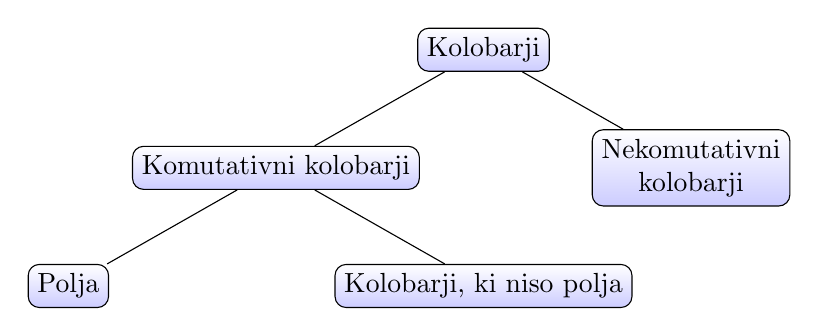
\begin{tikzpicture}[sibling distance=15em,
  every node/.style = {shape=rectangle, rounded corners,
    draw, align=center,
    top color=white, bottom color=blue!20}]]
  \node {Kolobarji}
    child { node {Komutativni kolobarji}
      child { node {Polja} }
      child { node {Kolobarji, ki niso polja} }
    }
    child { node {Nekomutativni \\ kolobarji} };
\end{tikzpicture}
\\
\\
\begin{example}
\begin{example_case}
$\mathbb{Z}$ (tipičen primer kolobarja)
\end{example_case}
\begin{example_case}
$\mathbb{Q}, \mathbb{R}, \mathbb{C}$ (to niso tipični primeri kolobarjev, saj so kar polja)
\end{example_case}
\begin{example_case}
\textbf{Trivialni} ali \textbf{ničelni kolobar}:
$$\{0\}$$
\end{example_case}
\begin{statement}
$$\text{Kolobar} \ \mathcal{K} \ \text{je ničelen} \iff 1=0$$

\begin{proof}\leavevmode \\
$\implies$: Očitno\\
$\impliedby$: $\forall x \in \mathcal{K}. \ x = 1x = 0x = 0$
\end{proof}
\end{statement}
\begin{example_case}
Matrični kolobarji ($M_{n}(\mathbb{R})$, $M_{n}(\mathbb{C})$) z običajnim seštevanjem in množenjem,
$$0 =
	\underbrace{\begin{bmatrix} 
		0 & 0 & \cdots & 0 \\
		0 & \ddots & \ddots & \vdots \\
		\vdots & \ddots & \ddots & 0 \\
		0 & \cdots & 0 & 0		
	\end{bmatrix}}_n; \ 
		1 =	\underbrace{\begin{bmatrix} 
		1 & 0 & \cdots & 0 \\
		0 & \ddots & \ddots & \vdots \\
		\vdots & \ddots & \ddots & 0 \\
		0 & \cdots & 0 & 1
	\end{bmatrix}}_n
$$
Ta kolobar je nekomutativen za $n \geq 2$\\
$ A = \begin{bmatrix}
		1 & 0 \\
		0 & 0
	  \end{bmatrix}
$;
$ B = \begin{bmatrix}
		0 & 1 \\
		0 & 0
	  \end{bmatrix}
$	
$\implies$
$AB = B, \ BA = 0$ \\
$A$ in $B$ ne komutirata, prav tako pa smo videlo da je lahko produkt dveh neničelnih elementov $0$.
\end{example_case}

\begin{definition}
\label{def:left_zero_divisor}
Element $x \neq 0$ kolobarja $\mathcal{K}$, je \textbf{levi delitelj niča}, če obstaja tak $y \neq 0, \in  \mathcal{K}$, da velja: $xy = 0$.
\end{definition}

\begin{definition}
\label{def:right_zero_divisor}
Element $x \neq 0$ kolobarja $\mathcal{K}$, je \textbf{desni delitelj niča}, če obstaja tak $y \neq 0, \in  \mathcal{K}$, da velja: $yx = 0$.
\end{definition}

\begin{definition}
Element $x$ je \textbf{delitelj niča}, če je \textbf{hkrati levi in desni delitelj niča}.
\end{definition}

\begin{remark}
\begin{equation}
\label{eq:left_zero_divisor_iff_right}
\mathcal{K} \ \text{ima leve deljitelje niča} \iff \mathcal{K} \  \text{ima deljitelje niča}
\end{equation}
\begin{proof}\leavevmode \\
$\implies$: Obstajata taka $y \neq 0, x \neq 0$, da je $xy = 0$. Imamo dve možnosti
\begin{enumerate}
\item $yx=0 \implies$ Dokaz je končan.
\item $yx \neq 0$: $x(yx) = 0 = (yx)y$ in je $yx$ desni delitelj niča .
\end{enumerate} 
$\impliedby$: Očitno.
\end{proof}
\end{remark}

V \textbf{Kolobarju brez deliteljev niča} velja:
\begin{equation}
\label{eq:xy_is_zero_implies_one_zero}
\forall x,y \in \mathcal{K}. \ xy = 0 \implies x = 0 \lor y = 0
\end{equation}

V takih kolobarjih velja pravilo krajšanja:
$$ xy = xz \land x  \neq 0 \implies y = z$$
$$ yx = zx \land x  \neq 0 \implies y = z$$
$$ xy = xz \iff x(y-z) = 0$$
$$ yx = zx \iff (y-z)x = 0$$
\end{example}

Kolobar je monoid za množenje zato lahko govorimo o obrnljivih elementih.
\begin{example}
\begin{example_case}
V $\mathbb{Z}$ sta obrnljiva $1, -1$.
\end{example_case}
\begin{example_case}
V $\mathbb{Q}, \mathbb{R}, \mathbb{C}$ so obrnljivi vsi elementi razen $0$
\end{example_case}
\end{example}

\begin{definition}
\label{def:skew_field}
Kolobar, v katerem $1 \neq 0$ in v katerem so \textbf{vsi neničelni elementi obrnljivi} se imenuje \textbf{obseg}.
\end{definition}

\begin{definition}
\label{def:field}
Komutativni obseg se imenuje \textbf{polje}
\end{definition}

\begin{example}
\begin{example_case}
$\mathbb{Q}, \mathbb{R}, \mathbb{C}$, so polja
\end{example_case}
\begin{example_case}
Nekomutativne obsege bomo dodali kasneje
\end{example_case}
\end{example}

\begin{statement}
\label{st:invertible_element_is_not_zero_divisor}
Obrnljiv element kolobarja ni levi(ali desni) delitelj niča.\\
Obsegi so zato kolobarji brez deliteljev niča.
\end{statement}
\begin{proof}
$x$ je obrnljiv: $xy=0$\\
$y = 1y = (x^{-1}x)y =  x^{-1}(xy) = x^{-1}0 = 0$ Torej $x$ ni delitelj niča.
\end{proof}

\subsection{Vektorski prostori}

\begin{definition}
\label{def:vector_space}
Naj bo $\mathcal{F}$ polje. Množica $\mathcal{V}$ skupaj z (notranjo) binarno operacijo seštevanje $+: \mathcal{V} \times \mathcal{V} \to \mathcal{V}$ in zunanjo binarno operacijo $\mathcal{F} \times \mathcal{V} \to \mathcal{V}$ imenovano \textbf{množenje s skalarji} in označeno z $(\lambda, v) \mapsto \lambda v$, se imenuje \textbf{vektorski prostor nad poljem $\mathcal{F}$}, če zanj velja:
\begin{enumerate}[label=\subscript{V}{\arabic*}:]
\item Za seštevanje je $\mathcal{V}$ Abelova grupa
\item Velja distributivnost v vektorskem faktorju
\begin{equation}
\label{eq:vector_space_vector_distributivity}
\forall \lambda \in \mathcal{F}. \  \forall u,v \in \mathcal{V}. \ \lambda(u+v) = \lambda u + \lambda v
\end{equation}
\item Velja distributivnost v skalarnem faktorju
\begin{equation}
\label{eq:vector_space_scalar_distributivity}
\forall \lambda, \mu \in \mathcal{F}. \  \forall v \in \mathcal{V}. \ (\lambda +\mu)v = \lambda v + \mu v
\end{equation}
\item Velja zakon homogenosti
\begin{equation}
\label{eq:vector_space_homogenous}
\forall \lambda, \mu \in \mathcal{F}. \  \forall v \in \mathcal{V}. \ (\lambda \mu)v = \lambda( \mu v)
\end{equation}
\item Enota
\begin{equation}
\label{eq:vector_space_unit}
 \forall v \in \mathcal{V}. \ 1v = v
\end{equation}
\end{enumerate}
\end{definition}

Za vsak vektorski prostor očitno veljajo naslednje trditve

\begin{itemize}
\item $$\forall \lambda \in \mathcal{F}. \ \lambda 0 = 0$$
\item $$\forall u,v \in \mathcal{V}. \  0x = 0$$
\item $$\forall \lambda, \mu \in \mathcal{F}. \  \lambda \mu = 0 \implies \lambda = 0 \lor \mu = 0$$
\item $$\forall \lambda, \mu \in \mathcal{F}. \ (-\lambda) \mu = \lambda(- \mu) = -(\lambda \mu) $$
\end{itemize}

\begin{remark}
Elementom polja $\mathcal{F}$ pravimo \textbf{skalarji}, elementom $\mathcal{V}$ pa vektorji
\end{remark}

\begin{itemize}
\item $\mathcal{F} = \mathbb{R}$: Realni vektorski prostor
\item $\mathcal{F} = \mathbb{C}$: Kompleksni vektorski prostor

\end{itemize}

\begin{example}
\begin{example_case}
Splošni prostor $\mathcal{F}^n$, kjer vpeljemo operaciji:\\
\textbf{Seštevanje}
\begin{equation}
\label{eq:vector_space_addition}
(u_1, u_2, \dots , u_n) + (v_1, v_2, \dots, v_n) \mapsto (u_1 + v_1, u_2 + v_2, \dots, u_n + v_n)
\end{equation}
\textbf{Množenje s skalarjem}
\begin{equation}
\label{eq:vector_space_scalar_multiplication}
\lambda (u_1, u_2, \dots , u_n) \mapsto (\lambda u_1 , \lambda u_2 , \dots, \lambda u_n)
\end{equation}
\end{example_case}
\begin{example_case}
Trivialni vektorski prostor: $\{0\}$
\end{example_case}
\begin{example_case}
Vektorski prostor polinomov stopnje največ $n$, kjer seštevanje in množenje definiramo na običajen način
\end{example_case}
\begin{example_case}
$\mathbb{C}$ je vektorski prostor nad $\mathbb{R}$ ( za $+$ je Abelova grupa, množenje pa definiramo po komponentah, tako je nad $\mathbb{R}$ to $2$-dimenzionalen, nad $\mathbb{C}$ pa $1$-dimenzionalen)
\end{example_case}
\end{example}

\subsection{Algebre}
Mnogi pomembni primeri kolobarjev so hkrati tudi vektorski prostori, dejansko so algebre.

\begin{definition}
\label{def:algebra}
Naj bo $\mathcal{F}$ polje (komutativen obseg). Množica $\mathcal{A}$ skupaj z (notranjima) binarnima operacijama $+$ (seštevanje) in $*$ (množenje) ter zunanjo binarno operacijo $\mathcal{F} \times \mathcal{A} \to \mathcal{A}$ (množenje s skalarji) je \textbf{Algebra na poljem $\mathcal{F}$ ali $\mathcal{F}$-algebra}, če velja:
\begin{enumerate}[label=\subscript{V}{\arabic*}:]
\item Za seštevanje in množenje s skalarji je $\mathcal{A}$ vektorski prostor
\item Za množenje je $\mathcal{A}$ monoid
\item Veljata neke vrste levi in desni distributivnostni zakon
$$\forall x,y,z \in \mathcal{A}. \ \forall \lambda, \mu \in \mathcal{F}. \ (\lambda x + \mu y) z = \lambda(xz) + \mu(yz)$$
$$\forall x,y,z \in \mathcal{A}. \ \forall \lambda, \mu \in \mathcal{F}. \ z(\lambda x + \mu y) = \lambda(zx) + \mu(zy)$$

\begin{remark}
Za $\lambda = \mu = 1$ je to navadna distributivnost. Torej je algebra kolobar, ki je hkrati vektorski prostor, v katerem velja še:
$$\lambda(xz) = (\lambda x)z = x(\lambda z)$$
\end{remark}

\end{enumerate}

\end{definition}


\begin{example}
\begin{example_case}
Vektorski prostor $\mathcal{F}^n$ postane algebra, če definiramo množenje, najlažje kar po komponentah:
\begin{equation}
\label{eq:vector_space_to_algebra_component_mulitplication}
(x_1, x_2, \dots, x_n) (y_1, y_2, \dots, y_n) \mapsto (x_1 y_1,, x_2 y_2, \dots, x_n y_n)
\end{equation} 
\end{example_case}
\begin{example_case}
Kolobar $M_n(\mathbb{R})$ postane algebra, če definiramo množenje s skalarji
\begin{equation}
\label{eq:matrix_scalar_multiplication}
\lambda (a_{ij}) = (\lambda a_{ij})
\end{equation}
\end{example_case}
\begin{example_case}
Vektorski prostor polinomov postane algebra, če vpeljemo množenje polinomov na standardni način
\end{example_case}
\end{example}

\begin{remark}
'Teorija kolobarjev' in 'teorija kolobarjev in algeber' se razlikujeta zgolj v poudarku.
\end{remark}

\subsection{Podgrupe, podkolobarji in druge podstrukture}
$(\mathbb{R}, +)$ in $(\mathbb{C}, +)$ sta različni strukturi, a očitno povezani Abelovi grupi. Operacija je seštevanje in $\mathbb{R} \subseteq \mathbb{C}$. Rečemo: $(\mathbb{R}, +)$ je podgrupa $(\mathbb{C}, +)$. \\
Podobno rečemo 
$(\mathbb{R}, +, *)$ je podkolobar $(\mathbb{C}, +, *)$\\
In ker sta to tudi polji rečemo kar kar $(\mathbb{R}, +, *)$ je podpolje $(\mathbb{C}, +, *)$\\

\subsubsection{Podgrupe}

\begin{definition}
\label{def:subgroup}
\textbf{Neprazna} podmnožica $\mathcal{H}$ grupe $\mathcal{G}$ je \textbf{podgrupa} grupe $\mathcal{G}$, če je za isto operacijo (zožitev na $\mathcal{H} \times \mathcal{H}$) tudi sama grupa. 
\end{definition}

\begin{example}
\begin{example_case}
Vsaka grupa $\mathcal{G}$ ima vsaj dve podgrupi: $\mathcal{G}$ in $\{1\}$\\
\begin{remark}
$\{1\}$ se imenuje \textbf{trivialna podgrupa}
\end{remark}

\begin{remark}
Vsaka od $\mathcal{G}$ različna podgrupa se imenuje \textbf{prava podgrupa}
\end{remark}
\end{example_case}

\end{example}

\begin{statement}
\label{st:subgroup_equivalent_defintions}
Za neprazno podmnožico $\mathcal{H}$ grupe $\mathcal{G}$ so naslednje trditve ekvivalentne:
\begin{enumerate}[label=(\roman*)]
\item $$\mathcal{H} \ \text{je podgrupa} \ \mathcal{G}$$
\item $$\forall x,y \in \mathcal{H}. \ x y^{-1} \in \mathcal{H}$$ 
\item $$\forall x,y \in \mathcal{H}. \ x y \in \mathcal{H} \land x^{-1} \in \mathcal{H}$$ 
\end{enumerate}
\end{statement}
\begin{proof}
\label{pr:subgroup_equivalent_defintions}\leavevmode \\
(i) $\implies$ (ii) : Očitno iz definicije da je $\mathcal{H}$ grupa \\
(ii) $\implies$ (iii) : \\
$$x \in \mathcal{H} \Longrightarrow 1 = x x^{-1} \in \mathcal{H} \Longrightarrow x^{-1} = 1 x^{-1} \in \mathcal{H} \ \text{// Zaprta za inverz}$$
$$x,y \in \mathcal{H} \Longrightarrow x y = x (y^{-1})^{-1} \in \mathcal{H} \ \text{Zaprta za poljubna dva}$$
(iii) $\implies$ (i):\\
Očitno zaprta za množenje, asociativna, ker velja na večji množici ($\mathcal{G}$)
$$1 = x x^{-1} \in \mathcal{H}$$
$$x \in \mathcal{H} \implies x^{-1} \in \mathcal{H}$$
\end{proof}

Govorimo 'grupa $\mathcal{H}$' ali 'podgrupa $\mathcal{H}$' označimo:

$$\mathcal{H} \leq \mathcal{G}$$

\begin{example}
\begin{example_case}
$\mathbb{R} - \{0\}$ je podgrupa $(\mathbb{C}-\{0\})$
\end{example_case}
\begin{example_case}
$\{x \in \mathbb{R} | x < 0\}$ je podgrupa $(\mathbb{C}-\{0\})$
\end{example_case}
\begin{example_case}
$\{1, -1, i, -i\}$ je podgrupa $(\mathbb{C}-\{0\})$
\end{example_case}
\begin{example_case}
$\{z \in \mathbb{C} | \ |z| = 1\}$ je podgrupa $(\mathbb{C}-\{0\})$
\end{example_case}
\begin{example_case}
$\{x \in \mathbb{R} | \ |x| > 1\}$ \textbf{ni} podgrupa $(\mathbb{C}-\{0\})$
\end{example_case}
\begin{example_case}
$\{z \in \mathbb{C} - \{0\} | \ |z| \leq 1\}$ \textbf{ni} podgrupa $(\mathbb{C}-\{0\})$
\end{example_case}
\end{example}

\begin{remark}\\
V aditivni grupi velja \\(ii) :  $\forall x,y \in \mathcal{H}. \ x - y \in \mathcal{H}$ in \\
(iii): $\forall x,y \in \mathcal{H}. \ x + y \in \mathcal{H} \land -x \in \mathcal{H}$
\end{remark}
\\

\begin{example}
Podgrupe $(\mathbb{Z}, +)$\\
\begin{example_case}
Trivialna primera podgrup sta $\mathbb{Z}$ in $\{0\}$
\end{example_case}
\begin{example_case}
$2\mathbb{Z} = \{2n | n \in \mathbb{Z}\}$
\end{example_case}
\begin{example_case}
$k\mathbb{Z} = \{kn | n \in \mathbb{Z}\}$ // $k \in \mathbb{Z}$
\end{example_case}
\end{example}

\begin{definition}
\label{def:conjugate_elements_group}
Elementa $a, b$ iz grupe $\mathcal{G}$ sta si \textbf{konjugirana}, če velja:
\begin{equation}
\label{eq:conjugate_element_group}
\exists c \in \mathcal{G}. \ b = c a c^{-1}
\end{equation}
\begin{remark}
Relacija 'elementa sta si konjugirana' je ekvivalenčna.
\end{remark}
\end{definition}

\begin{statement}
\label{def:conjugate_subgroup}
Če je $c \in \mathcal{H} \leq \mathcal{G}$, je 
\begin{equation}
\label{eq:conjugate_subgroup}
c \mathcal{H} c^{-1} := \{ chc^{-1} | \ h \in \mathcal{H}\}
\end{equation}
\textbf{konjugirana podgrupa} podgrupe $\mathcal{H}$.
\end{statement}

\begin{proof}
\label{st:conjugate_subgroup_is_subgroup}
$$chc^{-1} c h' c^{-1} = c\underbrace{hh'}_{\in \mathcal{H}}c^{-1} \in \mathcal{H}$$
$$(chc^{-1})^{-1}  = (c^{-1})^{-1}h^{-1}c^{-1} = c \underbrace{h^{-1}}_{ \in \mathcal{H}} c^{-1} \in \mathcal{H}$$
\end{proof}

\begin{remark}
Pojem konjugiranih podgrup ima smisel v nekomutativnih grupah
\end{remark}

\subsubsection{Podkolobarji}

\begin{definition}
\label{def:sub_ring}
Podmnožica $\mathcal{L}$ kolobarja $\mathcal{K}$ je \textbf{podkolobar} kolobarja $\mathcal{K}$, če vsebuje enoto \{1\} kolobarja $\mathcal{K}$ in če je kolobar za isti operaciji. 
\end{definition}

\begin{example}
\begin{example_case}
$\mathcal{L} = \{ \begin{bmatrix}
		x & 0 \\
		0 & 0
	  \end{bmatrix} | \ x \in \mathbb{R}\}$\\
	  Sicer je kolobar za isti operaciji, a ne podeduje enote (ima svojo), torej \textbf{ni} podkolobar.
\end{example_case}
\end{example}

\begin{statement}
\label{st:sub_ring_closed_for_inverse}
Podmnožica $\mathcal{L}$ kolobarja $\mathcal{K}$ je podkolobar natanko tedaj, ko velja
\begin{equation}
\label{eq:sub_ring_closed_for_inverse}
1 \in \mathcal{L} \land 
\forall x, y \in \mathcal{L}. \ x-y \in \mathcal{L}
\end{equation}
\end{statement}

\begin{proof}\leavevmode \\
\label{pr:sub_ring_closed_for_inverse}
$\implies$: Sledi iz definicije\\
$\impliedby$ Iz predpostavke sledi, da je $\mathcal{L}$ podgrupa za $+$.\\ Prav tako je $(\mathcal{L}, *)$ monoid\\ Izpolnjevanje distributivnih zakonov pa sledi iz tega da so izpolnjeni tudi na $\mathcal{K}$
\begin{remark}
Uporabili smo trditev (\ref{st:subgroup_equivalent_defintions}) in (ii) pogoj zamenjali z (iii)
\end{remark}
\end{proof}

\begin{example}
\begin{example_case}
Kolobar $\mathbb{Z}$ je podkolobar $\mathbb{Q}$.
\end{example_case}
\begin{example_case}
Kolobar $\mathbb{Q}$ je podkolobar $\mathbb{R}$.
\end{example_case}
\end{example}

\subsubsection{Podprostori}
\begin{definition}
\label{def:vector_subspace}
Podmnožica $\mathcal{U}$ vektorskega prostora $\mathcal{V}$ je \textbf{podprostor} $\mathcal{V}$, če je za isti operaciji tudi sama vektorski prostor.
\end{definition}

\begin{statement}
Za neprazno podmnožico $\mathcal{U}$ vektorskega prostora $\mathcal{V}$ so naslednje trditve ekvivalentne
\begin{enumerate}[label=(\roman*)]
\item $$\mathcal{U} \ \text{je podprostor} \ \mathcal{V}$$
\item $$\forall x, y \in \mathcal{U}. \ \forall \lambda, \mu \in \mathcal{F}. \ \lambda x + \mu y \in \mathcal{U}$$
\item $$\forall x, y, \in \mathcal{U}. \  x + y \in \mathcal{U} \land \forall x \in \mathcal{U}. \  \forall \lambda \in \mathcal{F}. \ \lambda x  \in \mathcal{U}$$
\end{enumerate}	
\end{statement}

\begin{proof}
Očitno
\end{proof}

\begin{example}
Edini podprostori vektorskega prostora $\mathbb{R}^3$ so:
\begin{itemize}
\item $\{0\}$, $\mathbb{R}^3$
\item premice skozi izhodišče
\item ravnine skozi izhodišče
\end{itemize}
\end{example}

\subsubsection{Podalgebre}
\begin{definition}
\label{def:subalgebra}
Podmnožica $\mathcal{B}$ algebre $\mathcal{A}$ je \textbf{podalgebra} $\mathcal{A}$, če je za iste operacije tudi sama algebra in vsebuje enoto \{1\} iz algebre $\mathcal{A}$.
\end{definition}

\begin{statement}
Neprazna podmnožica $\mathcal{B}$ algebre $\mathcal{A}$ je \textbf{podalgebra} algebre $\mathcal{A}$ natanko tedaj ko zanjo velja:
\begin{equation}
\label{eq:is_subalgebra}
1 \in \mathcal{B} \land \forall x, y \in \mathcal{B}. \ \forall \lambda \in \mathcal{F}. \ \underbrace{x+y, \lambda x}_{podprostor}, xy \in \mathcal{B}
\end{equation}
Torej je zaprta za seštevanje, množenje in množenje s skalarji
\end{statement}

\begin{proof}
Enako kot za podkolobarje
\end{proof}

\begin{example}
\begin{example_case}
$A = \mathcal{M}_2(\mathbb{R})$, 
$B = \{ \begin{bmatrix}
		a_{11} & a_{12} \\
		0 	   & a_{22}
	  \end{bmatrix} | a_{ij} \in \mathbb{R} \}$
\leavevmode
\end{example_case}
\end{example}

\subsubsection{Podpolje}

\begin{definition}
\label{def_subfield}
Podmnožica $\mathcal{F}$ polja $\mathcal{E}$ je \textbf{podpolje} polja $\mathcal{E}$, če je za isti operaciji tudi sama polje
\end{definition}

\begin{remark}
Podpolje nujno vsebuje isto enoto $1$ kot polje $\mathcal{E}$, naj bo $e \in \mathcal{F}$ enota.
$e^2 = e \implies e(\underbrace{1}_{enota \ \mathcal{E}}- \ e) = 0$ Ker v poljih ni deliteljev niča, velja $e=1$.
\end{remark}

\begin{statement}
Podmnožica $\mathcal{F} \neq \{0\}$ polja $\mathcal{E}$ je podpolje natanko tedaj ko velja
\begin{equation}
\label{eq:subfield_equivalent_definition}
\forall x, y \in \mathcal{F}. \ xy, x-y \in \mathcal{F} \land 0 \neq x \in \mathcal{F}. \ x^{-1} \in \mathcal{F} 
\end{equation}
\end{statement}

\begin{proof}Podobno kot prej
	
\end{proof}

\begin{statement}
$\mathcal{F} = \{0\} \iff 1 = 0$
\begin{proof}\leavevmode\\
$\implies$

$\forall x \in \mathcal{F}. \ 0x = x$ torej je $0$ nevtralni element

$\impliedby$

$\forall x \in \mathcal{F}. \ x = 1x = 0x = 0$ vsi elementi so ničelni
\end{proof} 
\end{statement}


\begin{definition}
\label{def:field_extension}
Polje $\mathcal{E}$ je \textbf{razširitev} polja $\mathcal{F}$ če je $\mathcal{F}$ podpolje $\mathcal{E}$.
\end{definition}

\begin{example}
\begin{example_case}
$\mathbb{R}$ je podpolje $\mathbb{C}$
\end{example_case}
\begin{example_case}
$\mathbb{C}$ je razširitev $\mathbb{R}$, ki je razširitev $\mathbb{Q}$
\end{example_case}
\end{example}


\subsubsection{Logične operacije nad (pod)strukturami}
Če so $\mathcal{H}_i$ podgrupe grupe $\mathcal{G}$ je tudi njihov presek $\cap \mathcal{H}_i$ podgrupa.

\begin{remark}
Družina $\mathcal{H}_i$ je \textbf{lahko končna ali neskončna} torej poljubna
\end{remark}\\

\textbf{Presek} algebrskih struktur (podgrup, podkolobarjev, podprostorov, podalgeber, podpolj) \textbf{ohrani lastnosti} te algebrske strukture.\\

\textbf{Unija} algebrskih struktur praviloma \textbf{ne ohrani} lastnosti te algebrske strukture.

\begin{example}
\begin{example_case}
$2\mathbb{Z} = \{2n | n \in \mathbb{Z}\}$ in $3\mathbb{Z} = \{3n | n \in \mathbb{Z}\}$ sta podgrupi $\mathbb{Z}$, njuna unija pa ni podgrupa (saj ni grupa), ker $2+3=5 \notin 2\mathbb{Z} \cup 3\mathbb{Z}$
\end{example_case}
\end{example}

\subsection{Generatorji}
$\mathbb{R}^3$ je generiran z vektorji: $(1,0,0), (0,1,0), (0,0,1)$. Edini podprostor, ki te vektorje vsebuje je namreč $\mathbb{R}^3$ sam. Seveda je generiran tudi z drugimi vektorji: $(1,1,0), (0,1,0), (0,0,1)$.\\
Vektorja $(1,0,0),(0,1,0)$ pa generirata ravnino: $z=0$.

\subsubsection{Generatorji grup}
Naj bo $\mathcal{X}$ neprazna podmnožica grupe $\mathcal{G}$, Vzemimo množico vseh elementov oblike $x_1 x_2 \dots x_n$, kjer velja $x, x^{-1} \in \mathcal{X}$ in jo označimo z $<\mathcal{X}>$.
 
Če je $\mathcal{X} = \{y_1, y_2, \dots , y_n\}$ pišemo tudi $\mathcal{X} = <y_1, y_2, \dots , y_n>$. 

Tako $<x,y>$ sestoji iz elementov kot so: $1, x, y, x^2, x^3, x^{-1}, x^{-2}, x^{-1}y, y^{-1}, x^5y^{-1}x^3y^{-3}xy^2, \dots$
\textbf{Opazimo}, da je $<\mathcal{X}>$ podgrupa
$$u,v \in <x> \implies uv \in <\mathcal{X}> \land u^{-1} \in <x>$$
$(x_1,\dots, x_n)^{-1} = x_{1}^{-1} \dots x_n^{-1}$, ki vsebuje množico $\mathcal{X}$.

Velja pa tudi obratno: vsaka podgrupa grupe $\mathcal{G}$, ki vsebuje $\mathcal{X}$ vsebuje tudi to podgrupo($<\mathcal{X}>$).

Torej je $<\mathcal{X}>$ najmanjša podgrupa, ki vsebuje $\mathcal{X}$. Pravimo ji \textbf{podgrupa, generirana z $\mathcal{X}$}.

Če velja $<\mathcal{X}> = \mathcal{G}$, rečemo, da je $\mathcal{G}$ generirana z množico $\mathcal{X}$, elemente iz $\mathcal{X}$ pa imenujemo \textbf{generatorji} grupe $\mathcal{G}$, množici $\mathcal{X}$ pa \textbf{množica generatorjev}.\\

\begin{example}
\begin{example_case}
$\mathbb{Q}^+$ je grupa za množenje. Velja: $<\mathbb{N}> = \mathbb{Q}^+$
\end{example_case}
\begin{example_case}
$<2,3> = \{2^i 3^j | i,j \in \mathbb{Z}\}$
\end{example_case}
\end{example}

\begin{remark}
V aditivni grupi $<\mathcal{X}>$ za komponiranje elementov uporabljamo drugo operacijo, vse ostalo ostane isto.
\end{remark}\\

\begin{example}
\begin{example_case}
Grupa $(\mathbb{Z}, +)$ je generirana z $<1>$ in prav tako tudi z $<-1>$. Velja $\mathbb{Z} = <1> = <-1>$.
\end{example_case}
\end{example}

\begin{remark}
Grupe generirane z enim samim elementom imenujemo \textbf{ciklične}.($<2> = <4,6> = 2\mathbb{Z}$)

\end{remark}

Cilj je poiskati najmanjše množice generatorjev(očitno $<\mathcal{G}> = \mathcal{G}$).

\begin{definition}
\label{def:finitly_generated_group}
Grupa je \textbf{končno generirana} če je generirana s kako končno množico.
\end{definition}

\subsubsection{Generatorji kolobarja}
Naj bo $\mathcal{K}$ kolobar, $\emptyset \neq \mathcal{X} \subseteq \mathcal{K}$.

Označimo z $\overline{\mathcal{X}}$ podgrupo za seštevanje $\mathcal{K}$, ki vsebuje vse produkte elementov iz $\mathcal{X} \cup \{1\}$.

Opazimo: $\overline{\mathcal{X}}$ je podkolobar, ki vsebuje $\mathcal{X}$ in je vsebovan v vsakem podkolobarju, ki $\mathcal{X}$ vsebuje. Zato mu rečemo \textbf{podkolobar generiran z množico $\mathcal{X}$}.

\begin{example}
\begin{example_case}
$\mathcal{K} = \mathbb{C}$
\begin{itemize}
\item $\overline{\{1\}} = \mathbb{Z}$
\item $\overline{\{i\}} = \{ n + mi | n,m \in \mathbb{Z}\} = \mathbb{Z}[i]$ (Kolobar \textbf{Gaussovih celih števil})
\end{itemize}\leavevmode
\end{example_case}
\end{example}

\begin{remark}
Pojme, kot so \textbf{generator kolobarja, končno generiran kolobar,\dots} definiramo enako kot za grupo.
\end{remark}

\subsubsection{Generatorji vektorskih prostorov}

\begin{definition}
\label{def:linear_combination}
Naj bo $\mathcal{V}$ vektorski prostor nad $\mathcal{F}$. Vsakemu vektorju $v$ oblike
\begin{equation}
\label{eq:linear_combination}
v = \lambda_1 v_1 + \dots + \lambda_n v_n; \lambda_i \in \mathcal{F} \land v_i \in \mathcal{V}
\end{equation}
pravimo \textbf{linearna kombinacija} vektorjev $v_1, v_2, \dots, v_n$.
\end{definition}


\begin{definition}
\label{def:linear_spang_enerated}Naj bo 
$\emptyset \neq \mathcal{X} \subseteq \mathcal{V}$. Podprostor generiran z $\mathcal{X}$, torej podprostor, ki $\mathcal{X}$ vsebuje in je vsebovan v vsakem podprostoru, ki vsebuje $\mathcal{X}$, je množica $\mathcal{L}(\mathcal{X})$, vseh linearnih kombinacij vektorjev iz $\mathcal{X}$, $\mathcal{L}(\mathcal{X})$ imenujemo \textbf{linearna lupina množice $\mathcal{X}$}.
\end{definition}


\begin{definition}
Naj bo $\mathcal{X}$ množica generatorjev za $\mathcal{V}$, tedaj $\mathcal{X}$ imenujemo \textbf{ogrodje $\mathcal{V}$}. Velja še $\mathcal{L}(\mathcal{X}) = \mathcal{V}$.
\end{definition}

\begin{remark}
Posebnost vektorskega prostora je v tem, da imamo pojem \textbf{linearne neodvisnosti}, preko katerega vpeljemo pojem \textbf{baze} vektorskega prostora.
\end{remark}


\subsubsection{Generatorji algeber}

\begin{definition}
\label{def:subalgebra_generated}
Naj bo $\mathcal{A}$ algebra na $\mathcal{F}$, naj bo $\emptyset \neq \mathcal{X} \subseteq \mathcal{A}$. \textbf{Podalgebra generirana z $\mathcal{X}$} je množica, ki sestoji iz elementov $x$ oblike
\begin{equation}
\label{eq:subalgebra_generated_element}
x = \lambda_1 x_{11} x_{12} \dots x_{1n_1} + \dots + \lambda_r x_{r1} x_{rn_r}; \lambda_i \in \mathcal{F} \land x_i \in \mathcal{X} \cup \{1\}
\end{equation}
\end{definition}



\begin{example}
\begin{example_case}
$\mathcal{A} = \mathcal{M}_2(\mathbb{R})$ 
\begin{itemize}
\item Podalgebra generirana z:

$e_{11} = \begin{bmatrix}
		1 & 0 \\
		0 & 0
	  \end{bmatrix}$, 
$e_{22} = \begin{bmatrix}
		0 & 0 \\
		0 & 1
	  \end{bmatrix}$
	  
je algebra diagonalnih matrik: 
$$\begin{bmatrix}
	   \lambda & 0 \\
		0 & \mu
		
	  \end{bmatrix}; \ \lambda, \mu \in \mathbb{R}$$ 
\item Podalgebra generirana z:

$e_{11} = \begin{bmatrix}
		0 & 1 \\
		0 & 0
	  \end{bmatrix}$, 
$e_{22} = \begin{bmatrix}
		0 & 0 \\
		1 & 0
	  \end{bmatrix}$
	  
pa je celotna algebra $\mathcal{M}_2(\mathbb{R})$ (torej je generirana samo z dvema elementoma).

Ker velja:

$e_{12} e_{21} = e_{11}$ in $e_{21} e_{12} = e_{22}$, vidimo, da $e_{12}, e_{21}$ generirata algebro $\mathcal{M}_2(\mathbb{R})$.  
$\{e_{12}, e_{21}, e_{11}, e_{22} \}$ je baza algebre $\mathcal{M}_2(\mathbb{R})$

\begin{remark}

Za primerjavo: podkolobar $\mathcal{M}_2(\mathbb{R})$ generiran z $e_{12}$ in $e_{21}$ pa je 

$\mathcal{M}_2(\mathbb{Z})= \begin{bmatrix}
		u_{11} & u_{12} \\
		u_{21} & u_{22}
	  \end{bmatrix}; u_{ij} \in \mathbb{Z}$
\end{remark}
\end{itemize}\leavevmode
\end{example_case}
\end{example}

\subsubsection{Generatorji podpolj}
\begin{definition}
\label{def:subfield_generated}
Naj bo $\mathcal{X} \neq \emptyset$ podmnožica polja $\mathcal{F}$. \textbf{Podpolje generirano z $\mathcal{X}$} je množica
\begin{equation}
\label{eq:subfield_genrated_element}
\{uv^{-1} | u,v \in \overline{\mathcal{X}} \land v \neq 0\}
\end{equation}
\end{definition}

\begin{remark}
Podkolobar $\overline{\mathcal{X}}$ generiran z $\mathcal{X}$ ni nujno polje.
\end{remark}

Očitno vsako podpolje, ki $\mathcal{X}$ vsebuje, vsebuje tudi podpolje generirano z $\mathcal{X}$, toda zakaj ta množica je podpolje?.

Pomembno je dokazati, da je podgrupa za seštevaje (zaprtost za množenje, inverz, in 1 so očitne)
\begin{statement}
\label{st:generated_subfield_is_subgroup}
$$uv^{-1} - wz^{-1} = \underbrace{(uz - vw)}_{\in \overline{\mathcal{X}}} \underbrace{(vz)^{-1}}_{\in \overline{\mathcal{X}}}$$
\end{statement} 

\begin{example}
$\mathcal{F} = \mathbb{C}$

\begin{example_case}
$\mathcal{X} = \{1\}$ Podpolje generirano z $\mathcal{X}$ je $\mathbb{Q}$, medtem, ko $\overline{\mathcal{X}} = \mathbb{Z}$
Vsako podpolje $\mathbb{C}$ vsebuje $1$ in zato vsako podpolje vsebuje tudi $\mathbb{Q}$
\end{example_case}
\begin{example_case}
$\mathcal{X} = {i}$:  $\overline{\mathcal{X}} = \mathbb{Z}[i]$(Gaussova cela števila), podpolje generirano z $\mathcal{X}$ je 
\begin{equation}
\label{eq:rational_imag_generated}
\mathbb{Q}[i] := \{p + qi | p,q \in \mathbb{Q}\}
\end{equation}
\end{example_case}
\end{example}

\begin{remark}
Med drugim smo pokazali, da najmanjša podgrupa (podkolobar $\dots$), ki vsebuje dano množico, res obstaja. Zadevo pa lahko dokažemo tudi hitreje, tako da vzamemo presek vseh podstruktur, ki to strukturo vsebujejo.
\end{remark}

\subsection{Direktni produkti in vsote}
Iz danih struktur lahko konstruiramo nove na različne načine.
\subsubsection{Direktni produkti grup}

\begin{definition}
\label{def:outer_direct_product_of_groups}
Naj bodo $\mathcal{G}_1, \dots, \mathcal{G}_n$ grupe. Grupi $$\mathcal{G} := \mathcal{G}_1 \times \dots \times \mathcal{G}_n$$ ki jo dobimo kot kartezični produkt teh grup, pravimo \textbf{(zunanji) direktni produkt}.
\end{definition}

\begin{remark}
Da je ta struktura res grupa, operacijo definiramo po komponentah. Brez težav se prepričamo, da je to res grupa.
$$(x_1, x_2, \dots, x_n) * (y_1, y_2, \dots, y_n) := (x_1 y_1, x_2 y_2, \dots, x_n y_n)$$
Očitno:
$$1 = (1,1, \dots, 1)$$
$$(x_1, x_2, \dots, x_n)^{-1} = (x_1^{-1}, x_2^{-1}, \dots, x_n^{-1})$$
\end{remark}

\begin{remark}
Če so vse grupe v produktu aditivne, potem namesto $\mathcal{G} := \mathcal{G}_1 \times \dots \times \mathcal{G}_n$ pišemo $\mathcal{G} := \mathcal{G}_1 \oplus \dots \oplus \mathcal{G}_n$ in govorimo o \textbf{(zunanji) direktni vsoti grup}.
\end{remark}

\subsubsection{Direktni produkti kolobarjev}

\begin{definition}
\label{def:outer_direct_product_of_rings}
Naj bodo $\mathcal{K}_1, \dots, \mathcal{K}_n$ kolobarji. Kolobarju $$\mathcal{K} := \mathcal{K}_1 \times \dots \times \mathcal{K}_n$$ ki ga dobimo kot kartezični produkt teh kolobarjev, pravimo \textbf{(zunanji) direktni produkt}.
\end{definition}

\begin{remark}
Da je ta struktura res kolobar, operacijo definiramo po komponentah. Brez težav se prepričamo, da je to res kolobar.
$$(x_1, x_2, \dots, x_n) + (y_1, y_2, \dots, y_n) := (x_1 + y_1, x_2 + y_2, \dots, x_n + y_n)$$
$$(x_1, x_2, \dots, x_n) * (y_1, y_2, \dots, y_n) := (x_1 y_1, x_2 y_2, \dots, x_n y_n)$$
\end{remark}

\begin{remark}
Temu rečemo tudi \textbf{direktna (zunanja) vsota kolobarjev}.
\end{remark}

\subsubsection{Direktna vsota vektorskih prostorov}

\begin{definition}
\label{def:direct_sum_of_vector_spaces}
Naj bodo $\mathcal{V}_1, \dots, \mathcal{V}_n$ vektorski prostori nad $\mathcal{F}$. Vektorskemu prostoru $$\mathcal{V} := \mathcal{V}_1 \times \dots \times \mathcal{V}_n$$ ki ga dobimo kot kartezični produkt teh vektorskih prostorov, pravimo \textbf{direktna vsota} prostorov $\mathcal{V}_1, \dots, \mathcal{V}_n$ in ga označujemo kot $\mathcal{V}_1 \oplus \dots \oplus \mathcal{V}_n$.
\end{definition}

\begin{remark}
Da je ta struktura res vektorski prostor, operacijo definiramo po komponentah. Brez težav se prepričamo, da je to res vektorski prostor.
$$(x_1, x_2, \dots, x_n) + (y_1, y_2, \dots, y_n) := (x_1 + y_1, x_2 + y_2, \dots, x_n + y_n)$$
$$\lambda(x_1, x_2, \dots, x_n) := (\lambda x_1, \lambda x_2, \dots, \lambda x_n)$$
\end{remark}

\begin{remark}
$\mathcal{F}^{n}$ je direktna vsota $n$-kopij enorazsežnega prostora $\mathcal{F}$
\end{remark}



\subsubsection{Direktni produkt algebr}

\begin{definition}
\label{def:direct_product_of_vector_algebras}
Naj bodo $\mathcal{A}_1, \dots, \mathcal{A}_n$ algebre nad $\mathcal{F}$. Algebri $$\mathcal{A} := \mathcal{A}_1 \times \dots \times \mathcal{A}_n$$ ki jo dobimo kot kartezični produkt teh algebr, pravimo \textbf{direktni produkt}.
\end{definition}

\begin{remark}
Da je ta struktura res algebra, operacijo definiramo po komponentah. Brez težav se prepričamo, da je to res algebra.
$$(x_1, x_2, \dots, x_n) + (y_1, y_2, \dots, y_n) := (x_1 + y_1, x_2 + y_2, \dots, x_n + y_n)$$
$$(x_1, x_2, \dots, x_n) * (y_1, y_2, \dots, y_n) := (x_1 y_1, x_2 y_2, \dots, x_n y_n)$$
$$\lambda(x_1, x_2, \dots, x_n) := (\lambda x_1, \lambda x_2, \dots, \lambda x_n)$$
\end{remark}

\begin{remark}
Lahko govorimo tudi o direktnem produktu(direktni vsoti) neskončne družine struktur
\end{remark}

\begin{example}
\begin{example_case}
$\mathbb{R}$ glejmo kot algebro nad $\mathbb{R}$. Direktni produkt števno kopij z operacijami po komponentah je algebra $\mathbb{R} \times \mathbb{R} \times \dots$.

Operacije po komponentah točno sovpadajo z operacijami po komponentah za zaporedja. To je torej algebra realnih zaporedij.
\end{example_case}
\begin{example_case}
Naj bodo $\mathcal{F}_1, \dots, \mathcal{F}_n$ polja nad ne nujno istimi kolobarji. Definiramo operacije po komponentah in opazimo, da za $n \geq 2$ ima direktni produkt(polj ali kolobarjev) delitelje niča.
$$(x_1, 0, \dots , 0) * (0, x_2, x_3, \dots, x_n) = 0$$
\end{example_case}

\end{example}

\section{Primeri grup in kolobarjev}
\subsection{Cela števila}
Ker so $\mathbb{N}$ zgolj polgrupa za $+$, imamo v algebri raje $\mathbb{Z}$.

\begin{definition}
\label{def:total_ordering}
Množica $\mathcal{A}$ zadostuje \textbf{načelu dobre urejenosti}, če vsaka neprazna navzdol omejena podmnožica množice $\mathcal{A}$, vsebuje najmanjši element.
\end{definition}

\begin{remark}
Je ekvivalentno:

Če v množici $\mathcal{A}$, ki ustreza načelu dobre urejenosti, množica $\mathcal{B} \subseteq \mathcal{A}$ nima najmanjšega elementa, potem velja $\mathcal{B} = \emptyset$
\end{remark}

\begin{statement}
$\mathbb{N}$ ustreza načelu dobre urejenosti.
\end{statement}
\begin{proof}\leavevmode\\
Z indukcijo na $n$:
$n=1$: $1 \notin \mathbb{N}$

$n \implies n+1$: $1 \notin \mathbb{N}, 2 \notin \mathbb{N}, \dots, n \notin \mathbb{N} \underbrace{\implies}_{\text{Ker nima najmanjšega elementa}} n+1 \notin \mathbb{N}$
\end{proof}

Po indukciji isto velja tudi za $\mathbb{N} \cup \{0\}$, $\mathbb{N} \cup \{0, -1\}$, $\mathbb{N} \cup \{0, -1, -2\}$ $\dots$


Torej: Vsaka neprazna navzdol omejena podmnožica $\mathbb{Z}$ vsebuje najmanjše število.

Analogno: Vsaka neprazna navzgor omejena podmnožica $\mathbb{Z}$ vsebuje največje število.
\\

\begin{theorem}[Osnovni izrek o deljenju]
\label{th:fundamental_theorem_of_division}
Za poljubna $m,n \in \mathbb{Z}$ obstajata taki števili $p,q \in \mathbb{Z}$, da velja:
$$m = qn + r \land 0 \leq r < n$$
\end{theorem}

\begin{proof}
Vpeljimo
$$\mathcal{S}_{(n,m)} := \{k \in \mathbb{Z} | kn \leq m\}$$
Če $\mathcal{S} = \emptyset $ $\checkmark$ 
$\mathcal{S}$ je navzgor omejena, ker lahko najdemo tako število $k$, tako da je $kn > m$ in to velja tudi za vsako od $k$ večje število, zato $\mathcal{S}$ vsebuje največje število $q$. Tako velja
$$qn \leq m \ \ // \ \text{saj} \ q \in \mathcal{S}$$
$$(q + 1)n > m \ \ // \ \text{saj} \ (q + 1) \notin \mathcal{S}$$
$$r:= m-qn \geq 0$$
$$qn + n > m \ \ // \ \text{torej} \ n > r$$
\end{proof}

\begin{remark}
$r$ imenujemo \textbf{ostanek} pri deljenju $m$ z $n$.
\end{remark}
\\

$(\mathbb{Z}, +)$
Primeri podgrup

\begin{example}
\begin{example_case}
Trivialni primeri: $\{0\}$, $\mathbb{Z}$
\end{example_case}
\begin{example_case}
$n\mathbb{Z} = \{nk | k \in \mathbb{Z}\}$ // $n \in \mathbb{Z}$ je podgrupa za seštevanje

\begin{remark}
Ker $n\mathbb{Z} = (-n)\mathbb{Z}$, praviloma izberemo $n \in \mathbb{N}$
\end{remark}
\end{example_case}
\end{example}

\begin{theorem}
\label{th:only_aditive_subgroup_of_integers}Podmnožica $\mathcal{H}$ množice $\mathbb{Z}$ je podgrupa za seštevanje natanko tedaj, ko obstaja tak $n \geq 0$, da je $\mathcal{H} = n\mathbb{Z}$.
\end{theorem}

\begin{proof}\leavevmode\\
$\implies$\\
$\mathcal{H}$ je podgrupa $\mathbb{Z}$\\ $\mathcal{H} = \{0\} \implies n = 0$\\
$\mathcal{H} \neq \{0\}$, $k \in \mathcal{H} \iff -k \in \mathcal{H} \implies \mathcal{H} \cap \mathbb{N} \neq \emptyset$
Po načelu dobre urejenosti obstaja najmanjše število v $\mathcal{H}$, recimo mu $n$.\\
$n \in \mathcal{H} \implies n\mathbb{Z} \subseteq \mathcal{H} \ //\text{ker je podgrupa}$\\
Vzemimo sedaj: $m \in \mathcal{H} \implies \underbrace{r}_{\in \mathcal{H}} = \underbrace{m}_{\in \mathcal{H}} - \underbrace{qn}_{\in \mathcal{H}}$\\
In dobimo $r = 0$, ker iz $1 \leq r \leq n-1$ sledi, da $\mathcal{H}$ vsebuje od $n$ manjše število, kar je protislovje.\\
Torej
$m = qn \in \mathcal{H}$\\
$\impliedby$\\
$n\mathbb{Z}$ je podgrupa $\implies (nk - nl) = n(k-l) \in n\mathbb{Z}$

\end{proof}

\begin{definition}
\label{def:divisor_integers}
Naj bosta $m,k \in \mathbb{Z}$. Rečemo, da \textbf{$k$ deli $m$} (pišemo tudi $k|m$), če obstaja tak $q \in \mathbb{Z}$, da velja $m = qk$.
\end{definition}

\begin{remark}
Rečemo tudi $m$ \textbf{je deljiv} s $k$ ali $k$ je \textbf{delitelj} $m$. Prav tako uporabljamo $k \nmid m$, da povemo, da $k$ \textbf{ne deli} $m$.
\end{remark}


\begin{definition}
\label{def:gcd_integers}
Naj bosta $m,n \in \mathbb{Z}$, naravno število $d$ je \textbf{največji skupni delitelj} $m$ in $n$, če velja:
\begin{enumerate}
\item $d|m \land d|n$
\item $\forall d' \in \mathbb{N}. \ d'|m \land d'|n \implies d'|d \ //$ Vsak drugi skupni delitelj deli največji skupni delitelj
\end{enumerate} 
\end{definition}


\begin{remark}
Če sta $\mathcal{H}$ in $\mathcal{K}$ podgrupi aditivne grupe $\mathcal{G}$, je podgrupa tudi
$$\mathcal{H} + \mathcal{K} := \{h+k | h \in \mathcal{H}, k \in \mathcal{K}\}$$
Očitno $\mathcal{H}, \mathcal{K} \subseteq \mathcal{H} + \mathcal{K}$, to je tudi najmanjša podgrupa, ki vsebuje obe podgrupi.
\end{remark}

\begin{proof}
$$(h+k) - (h' + k') = (h - h') + (k - k') \in \mathcal{H} + \mathcal{K}$$
\end{proof}

\begin{theorem}
\label{th:existance_of_gcd}Za vsak par celih števil $m,n$, od katerih vsaj eno ni enako $0$, obstaja največji skupni delitelj $d$, ki ga označimo z $gcd(m,n)$, in je oblike $d= mx + ny$ za neka $x,y \in \mathbb{Z}$.
\end{theorem}

\begin{proof}
$m\mathbb{Z}$ in $n\mathbb{Z}$ sta podgrupi $\mathbb{Z}$, zato je tudi njuna vsota podgrupa. Po opombi zgoraj obstaja tak $d \in \mathbb{N}$, da velja $d\mathbb{Z} = m\mathbb{Z} + n\mathbb{Z}$ in ker eno izmed $m,n$ ni $0$ velja $d \neq 0$. Torej velja\\
$d = mx + ny$ za neka $x,y \in \mathbb{Z}$ Torej velja:\\ $d \mathbb{Z} \supseteq m\mathbb{Z} \implies m \in m\mathbb{Z} \subseteq d\mathbb{Z} \implies d|m$ in podobno za $n$.
Dokazali smo, da je $d$ skupni delitelj števil $m$ in $n$. Potrebno je še dokazati, da je največji.\\
Naj velja $c|m$ in $c|n$, potem $m=cz$ in $n=cw$.\\
Vemo da $d = mx + ny = c(zx + wy) \implies c|d$
\end{proof}

\begin{remark}
Dokaz za to se pojavi že v Evklidovi knjigi Elementi, približno 300 let pr. Kr.
\end{remark}

\begin{definition}
\label{def:coprime_integers}
Števili $m,n \in \mathbb{Z}$, ne obe enaki $0$, sta si \textbf{tuji}, če je njun največji skupni delitelj enak $1$. 
\end{definition}


\begin{corollary}
Celi števili $m,n$ sta si tuji natanko tedaj, ko obstajata taki celi števili $x,y$, ki zadostita enačbi:
$$1=mx + ny$$
\end{corollary}

\begin{proof}\leavevmode\\
$\implies$ \\Sledi iz izreka o obstoju največjega skupnega delitelja (\ref{th:existance_of_gcd})\\
$\impliedby$\\
$c|m \land c|n \implies c|1$ Torej je njun največji skupni delitelj 1 in sta si tuji. 
\end{proof}

\begin{remark}
Splošneje lahko definiramo največji skupni delitelj števil $n_1, n_2, \dots, n_k \in \mathbb{Z}$ na enak način ter njegovo eksistenco dokažemo na enak način ($d=n_1x_1 + n_2x_2 + \dots n_kx_k$). To seveda ne pomeni, da so si števila paroma tuja ($2,3,6$ so si tuja, ne pa tudi paroma tuja).
\end{remark}

\begin{definition}
\label{def:prime}
Naravno število $p$ je \textbf{praštevilo}, če sta $1$ in $p$ edini naravni števili, ki ga delita in velja $p \neq 1$.
\end{definition}

\begin{lemma}
\label{lem:prime_divisibility}
Naj bo $p$ praštevilo in $mn \in \mathbb{Z}$, tedaj velja:
$$p |mn \implies p|m \lor p|n$$
\end{lemma}

\begin{proof}
Predpostavimo, da $p\nmid m$.\\
$gcd(p,m) = 1 \implies 1 = px + my \implies n = pxn + \underbrace{mn}_{pz}y = p(xn + zy)$ \\
Podobno za drugo možnost.
\end{proof}

\begin{remark}
Tudi ta dokaz je bil poznan že Evklidu.
\end{remark}

\begin{theorem}[Osnovni izrek aritmetike]
\label{th:fundamental_theroem_of_arithmetics}Vsako naravno število $n \geq 2$ lahko zapišemo kot produkt praštevil. Ta zapis je do vrstnega reda faktorjev natančno enoličen.
\end{theorem}

\begin{proof}
Indukcija na $n$:\\
$n = 2 \ \checkmark$\\
$n-1 \implies n$\\
Če je $n$ praštevilo je dokaz zaključen. Če ni, ima vsaj dva delitelja ki nista $1$ ali $p$ (lahko sta enaka).\\
$n = kl;\  l,k < n$ \\
Po indukcijski predpostavki sta $l$ in $k$ produkta praštevil, torej je tudi $p$ produkt praštevil.\\
In še edinost zapisa:\\
$n = p_1 * p_2 * \dots * p_r = q_1 * q_2 * \dots * q_s$, produkt samih praštevil\\
$p_1 | q_1 * q_2 * \dots * q_s$ torej po lemi (\ref{lem:prime_divisibility}) deli natančno enega izmed faktorjev $q_i$. Brez škode za splošnost: $p_1|q_1 \underbrace{\implies}_{\text{ker sta praštevili}} p_1 = q_1$ Krajšamo s $p_1$ in nadaljujemo dokler ne pridemo do $1=1$.\\
Če pa imamo $s > r \implies q_{r+1}\dots q_s = 1$, kar pa je protislovje.
\end{proof}

\begin{theorem}
\label{th:infinite_number_of_primes}
Množica praštevil je neskončna.
\end{theorem}

\begin{proof}
Predpostavimo, da jih je končno, torej da so $p_1, p_2, \dots, p_n$ vsa praštevila. Tedaj $p_1*p_2*\dots * p_n + 1$ ni praštevilo in je zato gotovo deljivo z nekim praštevilom $p_i$.\\
$p_1*p_2*\dots * p_n + 1 = k*p_i \implies p_i(k - p_1*p_2*\dots *p_{i-1} * p_{i+1} * \dots * p_n) = 1$, protislovje.
\end{proof}

\subsection{Grupa in kolobar ostankov}

\begin{definition}
\label{def:modulo_congruent}
Celi števili $a$ in $b$ sta \textbf{kongruenti modulo $n$}, če $$n|(a-b)$$
\end{definition}

\begin{example}
\begin{example_case}
$13 \equiv  1 \ (\textrm{mod}\ 12)$, $21 \equiv -3 \ (\textrm{mod}\ 12)$
\end{example_case}
\begin{example_case}
$a \equiv b \ (\textrm{mod}\ 1)$
\end{example_case}
\end{example}

\begin{lemma}
\label{lem:modulo_equivalence_addition}
$$a \equiv a' \ (\textrm{mod}\ n) \land b \equiv b' \ (\textrm{mod}\ n) \implies a+b \equiv a'+b' \ (\textrm{mod}\ n) \land ab \equiv a'b' \ (\textrm{mod}\ n)$$
\end{lemma}

\begin{proof}
$$(a+b) - (a' + b') = \underbrace{(a-a') + (b-b')}_{\text{sta si kongruentna}}$$
$$(ab) - (a' b') = \underbrace{b(a-a') + a'(b-b')}_{\text{sta si kongruentna}}$$
\end{proof}

\begin{statement}
Relacija $a \equiv b \ (\textrm{mod}\ n)$ je ekvivalenčna:
\end{statement}

\begin{proof}\leavevmode\\
Refleksivna: $\checkmark$\\
Simetrična: $\checkmark$\\
Tranzitivna:\\
$a \equiv b \ (\textrm{mod}\ n)$ in $b \equiv c \ (\textrm{mod}\ n)$ $\implies c-a = \underbrace{(c-b) + (b-a)}_{\text{sta si kongruentna}}$
\end{proof}

Ker je relacija ekvivalenčna, lahko vpeljemo ekvivalenčne razrede. Z $[a]$ označimo ekvivalenčni razred, ki mu pripada $a$.

\begin{definition}
\label{def:equivalence_classes_modulo}
Ekvivalenčni razredi kongurgento z $n$ so:
$$\underbrace{[0]}_{\text{števila deljiva z }n} , \underbrace{[1]}_{\text{ostanek pri deljenji z }n \ \text{je }1}, \dots , [n-1]$$
in jih označimo z $\mathbb{Z}_n$.
%Se da tole kaj lepše zapisat, malce razpotegnjeno je vse, pa spodaj je dosti skupaj komentar.
\end{definition}

Potrebno je preveriti še dobro definiranost operacij.
\\
\\
\begin{statement}
Če v množici $\mathbb{Z}_n$ vpeljemo seštevanje:
\begin{equation}
\label{eq:def_modulo_adition}
[a] + [b] := [a+b]
\end{equation}
Postane $\mathbb{Z}_n$ Abelova grupa.
\end{statement}

\begin{proof}
Dobra definiranost seštevanja:\\
$$ \underbrace{[a] = [a']}_{a \equiv a' \ (\textrm{mod}\ n)} \land \underbrace{[b] = [b']}_{b \equiv b' \ (\textrm{mod}\ n)} \implies [a+b] = [a' + b']$$ 
Drugi del izjave pa je ekvivalenten: $a+b \equiv a' + b'\ (\textrm{mod}\ n)$, kar sledi iz leme (\ref{lem:modulo_equivalence_addition}).
\\\\
Preverimo še asociativnost:
$$([a] + [b]) + [c] = [a + b] + [c] \underbrace{=}_{\text{po definiciji}} \underbrace{[(a+b) + c] = [a + (b + c)] =}_{\text{asociativnost celih števil}} \dots = [a] + ([b] + [c])$$
Nevtralni element:
$$0 = [0]$$
Nasprotni element:
$$-[a] = [-a]$$
Komutativnost:
$$[a] + [b] = [a+b] = [b+a] = [b] + [a]$$
\end{proof}


\begin{statement}
Aditivna grupa $\mathbb{Z}_n$ postane\textbf{komutativen kolobar} $\mathbb{Z}_n$, če vpeljemo množenje s predpisom:
\begin{equation}
\label{eq:def_modulo_group_multiplication}
[a]*[b] := [a*b]
\end{equation}
\end{statement}

\begin{proof}\leavevmode\\
Dobra definiranost sledi iz leme(\ref{lem:modulo_equivalence_addition}), asociativnost in distributivnost pokažemo kot pri seštevanju (se sklicujemo na te lastnosti v celih številih).\\
Enota: $[1]$
\end{proof}


\begin{remark}
Da oznake poenostavimo, namesto $[a], 0 \leq a \leq n-1$ pišemo kar $a$, in tako $\mathbb{Z}_n = \{0,1, \dots, n-1\}$, pri čemer moramo obdržati v mislih, da to niso 'prava' cela števila.
\end{remark}

Vsoto $a+b$ izračunamo tako, da pogledamo ostanek pri deljenju običajne vsote, podobno s produktom.

\begin{example}
\begin{example_case}
V $\mathbb{Z}_{12}$: $3+4 = 7$ in $3+11 = 2 + 1*12 = 2$ ter $3*7 = 9$ in $3*8 = 0$.\\
$\mathbb{Z}_n$ ima torej lahko delitelje niča. Očitno je to res vedno, kadar je $n$ sestavljeno število. Če pa je $n$ praštevilo, pa to ni res, še več, $\mathbb{Z}_p$ je polje.
\end{example_case}
\end{example}

\begin{definition}
\label{def:full_ring}
Komutativen kolobar brez deliteljev niča se imenuje \textbf{cel kolobar}.
\end{definition}

\begin{example}
$\underbrace{\mathbb{Z}}_{\text{cel kolobar, ki ni polje}}, \mathbb{Q}, \mathbb{R}, \mathbb{C}$
\end{example}


\begin{statement}
\label{st:finite_full_ring_is_field}
Končen cel kolobar je polje.
\end{statement}

\begin{proof}Naj bo $\mathcal{K}$ končen cel kolobar. $0\neq a \in \mathcal{K} \implies a\ \text{je obrnljiv}$, naj bo $f: \mathcal{K} \to \mathcal{K}, f(x) = ax$. Potrebno je pokazati, da $1 \in \mathcal{Z}_f$\\ Dokazali bomo kar surjektivnost $f$, kar je v končnem polju ekvivalentno njeni injektivnosti.\\
$ax = ax \underbrace{\implies}_{\text{cel kolobar}} x=y$ torej $a(x-y) = 0 \land a \neq 0 \implies x = y$\\
Komutativnost(eksistenca levega inverza $\implies$ eksistenca desnega inverza $\implies$ eksistenca inverza)
\end{proof}

\begin{remark}
Izkaže se, da končnih nekomutativnih obsegov ni (dokaz je netrivialen).
\end{remark}

\begin{corollary}
Za vsako praštevilo $p$ je $\mathbb{Z}_p$ polje.
\end{corollary}

\begin{proof}
Zadošča pokazati, da $\mathbb{Z}_p$ nima deliteljev niča.\\
$a,b \in \mathbb{Z}_p, ab=0$. Torej je v običajnem produktu $ab$ večkratnik $p$, zato po lemi(\ref{lem:prime_divisibility}) $p$ deli vsaj eno, ker pa $a,b \in \{0,1,\dots, p-1\}$ velja $a = 0 \lor b=0$
\end{proof}

\subsection{Obseg kvaternionov}
Pojavi se naravno vprašanje, kako nadaljevati zaporedje:
$$\mathbb{N} \subset \mathbb{Z} \subset \mathbb{Q} \subset \mathbb{R} \subset \mathbb{C} \subset \ ?$$

\begin{definition}
\label{def:quaternion_element}

Vzemimo $4$-razsežen vektorski prostor nad $\mathbb{R}$, označimo ga s $\mathbb{H}$, njegovo bazo pa z $\{1, i, j, k\}$, tako dobimo značilni element
\begin{equation}
\label{eq:quaternion_element}
h := \lambda_0 + \lambda_1 i + \lambda_2 j + \lambda_3 k, \ \lambda_i \in \mathbb{R}
\end{equation}
Seštevanje in množenje s skalarji uvedemo enako kot pri normalnem $4$ razsežnem vektorskem prostoru. Elemente $\mathbb{H}$ imenujemo kvaternioni.
\end{definition}

\begin{remark}
$\mathbb{H}$ izhaja iz priimka irskega matematika, fizika in astronoma Sira Williama Rowana Hamiltona, ki jih je vpeljal leta 1843.
\end{remark}

\begin{definition}
\label{def:quaternion_multiplication}
Množenje vpeljemo po kosih in sicer: $1$ je enota za množenje, za druge pa velja:
\begin{equation}
\label{eq:quaternion_multiplication}
i^2 = j^2 = k^2 = ijk = -1
\end{equation}
Iz teh sledi: $$ij = -ji = k, jk = -kj = i, ki = -ik = j$$
\end{definition}
Ko poznamo množenje baznih elementov, lahko množimo tudi vse ostale.
\\
\\
\begin{statement}
S tako definiranim množenjem postane prostor $\mathbb{H}$ ne samo kolobar, ampak tudi algebra nad $\mathbb{R}$.
\end{statement}

\begin{remark}
Preverimo po definiciji.
\end{remark}

\begin{definition}
\label{def:conjuagate_quaternion}
\begin{equation}
\label{eq:conjugate_quaternion}
\overline{h} := \lambda_0 - \lambda_1 i - \lambda_2 j - \lambda_3 k
\end{equation}
\end{definition}

\begin{statement}
\label{st:inverse_quaternion}
Vsak neničelen kvaternion je obrnljiv in zanj velja 
\begin{equation}
\label{eq:inverse_quaternion}
h^{-1} = \frac{\overline{h}}{h\overline{h}}
\end{equation}
\end{statement}


\begin{proof}

Izračunamo:

$h \overline{h} = \lambda_0^2 + \lambda_1^2 + \lambda_2^2 + \lambda_3^2$\\
$h \neq 0 \implies h \overline{h} \in \mathbb{R} - \{0\}$, zato je vsak neničelen kvaternion obrnljiv in velja
$$h^{-1} = \frac{\overline{h}}{h\overline{h}}$$
\end{proof}

\begin{remark}
$\mathbb{H}$ je tako nekomutativen obseg.
\end{remark}

Lahko pa uporabljamo tudi drugačen zapis:
$\lambda_0 + \lambda_1 i + \lambda_2 j + \lambda_3 k $ pišemo $$(\lambda_0, \vec{u}), \vec{u} = \lambda_1 i + \lambda_2 j + \lambda_3 k$$
Množenje se tako glasi:
\begin{equation}
\label{eq:quaterion_vector_multiplication}
(\lambda_0, \vec{u}) * (\mu_0, \vec{v}) = (\lambda_0 \mu_0 - \vec{u} \vec{v}, \lambda_0\vec{v} + \mu_0\vec{u} + \vec{u} \times \vec{v})
\end{equation}

\begin{remark}
Množica $\{\pm 1, \pm i, \pm j, \pm k\}$ je antikomutativna grupa za množenje z osmimi elementi, ki ji rečemo tudi \textbf{kvaternionska grupa}.
\end{remark}


\subsection{Kolobar matrik}
$\mathcal{M}_n(\mathbb{R})$ in $\mathcal{M}_n(\mathbb{C})$ sta kolobarja (celo algebri).\\


\begin{statement}
Za vsak kolobar $\mathcal{K}$, je množica $\mathcal{M}_n(\mathcal{K})$ kolobar nad $\mathcal{K}$ za običajno seštevanje in množenje matrik.
\end{statement}

\begin{proof}
Preverimo po definiciji. $\mathcal{K}$ je lahko celo nekomutativen. Enota in ničeln element sta enaka kot pri $\mathcal{M}_n(\mathbb{R})$.
\end{proof}

$\mathcal{M}_n(\mathcal{K})$ je nekomutativen za $n \geq 2$ (za $n=1$ je kolobar matrik kar $\mathcal{K}$)


\begin{definition}
\label{def:idempotent_ring}
Element $e$ kolobarja $\mathcal{K}$ je \textbf{idempotent}, če zanj velja:
\begin{equation}
\label{eq:def_idempotent}
e^2 =  e
\end{equation}
\end{definition}

\begin{definition}
\label{def:nullpotent_ring}
Element $a$ kolobarja $\mathcal{K}$ je \textbf{nilpotent}, če zanj velja:
\begin{equation}
\label{eq:def_nullpotent}
\exists n \in \mathbb{N}. \ a^n =  0
\end{equation}
\end{definition}

\begin{example}
\begin{example_case}
Vsaka diagonalna matrika, z $0$ in $1$ na diagonali, je idempotent.
\end{example_case}
\begin{example_case}
Vsaka strogo zgoraj (ali spodaj) trikotna matrika je nilpotentna.
\end{example_case}
\end{example}

\begin{statement}
Naj bo $\mathcal{K}$ kolobar brez deliteljev niča in naj bo $e \in \mathcal{K}$ idempotent. Velja: $e = 1 \lor e = 0$.
\end{statement}

\begin{proof}
$e^2 = e \implies e(1-e) = 0 \underbrace{\implies}_{\text{ker nima deliteljev niča}} e = 1 \lor e = 0$
\end{proof}

\begin{statement}
$e$ je idempotent $\iff$ $1-e$ je idempotent
\end{statement}

\begin{proof}
Račun.
\end{proof}


Če je $\mathcal{K}$ algebra na poljem $\mathcal{F}$, tudi kolobar $\mathcal{M}_n(\mathcal{K})$ potem postane algebra, če definiramo:
$$\lambda (a_{ij}) := (\lambda a_{ij})$$

Poseben primer: $\mathcal{M}_n(\mathcal{F})$ je algebra na $\mathcal{F}$, $dim(\mathcal{M}_n(\mathcal{K}))= n^2$


\subsection{Kolobar funkcij}

Naj bo $\mathcal{X}$ množica in naj bo $\mathcal{K} = \{ f : \mathcal{X} \to \mathbb{R}\}$\\

$\mathcal{K}$ postane kolobar, če definiramo običajno seštevanje in množenje funkcij:
$$(f+g)(x) := f(x) + g(x) $$
$$(f*g)(x) := f(x) * g(x) $$
Skupaj z enoto: $e(x) = 1$ in nasprotnim elementom: $(-f)(x) = -f(x)$ 

\begin{example}
\begin{example_case}
Če je $\mathcal{X} = [a,b]$ ali $\mathbb{R}$, ipd., lahko govorimo o kolobarju $\mathcal{C}(x) = \{f: \mathcal{X} \to \mathcal{R} | \ f \ \text{zvezna} \}$. Res je kolobar, saj so vsote in produkti zveznih funkcij spet zvezne funkcije. Ne samo to, je tudi algebra.
\end{example_case}
\end{example}

Poznamo več primerov kolobarjev funkcij:
\begin{itemize}
\item odvedljive funkcije
\item omejene funkcije 
\item integrabilne funkcije 
\item polinomi (ta kolobar nima deliteljev niča).
\item $\dots$
\end{itemize}

Če v te kolobarje vpeljemo še množenje s skalarji:
\begin{equation}
\label{eq:def_scala_multiplication_functions}
(\lambda f) (x) = \lambda f(x)
\end{equation}

postanejo vsi ti kolobarji tudi algebre.
\\
\\
Na podoben način vpeljemo tudi kolobar (algebro) zaporedij $\mathcal{X} = \mathbb{N} \to \mathcal{A}$, kjer so vse operacije definirane po komponentah (seštevanje, množenje, množenje s skalarjem). Ter različne podalgebre (konvergentna zaporedja, omejena zaporedja, ...).

\begin{example}
\begin{example_case}
V algebri zveznih funkcij ($\mathcal{C}(\mathbb{R})$) je podalgebra generirana z $id(x) = x$ ravno algebra polinomov.
\end{example_case}
\end{example}


\subsection{Kolobar polinomov ene spremenljivke}
Vajeni smo, da je polinom funkcija, v algebri pa polinom obravnavamo kot formalen izraz.

\begin{definition}
\label{def:polynomial_in_algebra}
Polinom $p$ nad kolobarjem $\mathcal{K}$ je izraz oblike:
\begin{equation}
\label{eq:polynomial_in_algebra}
p(X) = a_0 + a_1 X + a_2 X^2 + \dots + a_n X^n, \  a_n \neq 0
\end{equation}
Kjer so $a_i \in \mathcal{K}$ t.i. koeficienti tega polinoma. 
\begin{itemize}
\item $a_0$ imenujemo \textbf{prosti (ali konstantni) člen}
\item $a_n$ (zadnji neničelen člen) imenujemo \textbf{vodilni člen (koeficient)}
\item $X$ imenujemo \textbf{spremenljivka}, a dejansko igra le formalno vlogo kot simbol
\end{itemize}
\end{definition}

Alternativno lahko polinom definiramo tudi kot

\begin{definition}
\label{def:polynomial_in_algebra_alternative_definition}
Polinom $p$ nad kolobarjem $\mathcal{K}$ je zaporedje elementov iz $\mathcal{K}$, ki je od nekega mesta naprej ničelno
\begin{equation}
\label{eq:def_polynomial_in_algebra_alterantive_definition}
p(n): \mathbb{N} \to \mathcal{K}, \ \exists n \in \mathbb{N}. \forall m \in \mathbb{N}. \ m > n \implies p(m) = 0 
\end{equation}
Torej:
$$p = (a_0, a_1, \dots , a_n, 0, 0, \dots )$$
Vendar pa ta definicija ni udobna za množenje.
\end{definition}

Da si prihranimo čas pri zapisu, spuščamo ničelne koeficiente: 
$$0 + 3X + 0x^2 - 5X = 3X - 5X^3$$

Udoben pa se nam zdi tudi zapis
$$p(X) = \sum_{k \geq 0} a_k X^k$$
Kjer se zavedamo, da od nekje naprej so vsi $a_k$ enaki $0$.

\begin{definition}[Seštevanje polinomov]
\label{def:polynomial_summation}
\begin{equation}
\label{eq:def_polynomial_equation}
\sum_{k \geq 0} a_k X^k + \sum_{k \geq 0} b_k X^k := \sum_{k \geq 0} (a_k + b_k) X^k
\end{equation}
\end{definition}

\begin{definition}[Množenje polinomov]
\label{def:polynomial_multiplication}
\begin{equation}
\label{eq:def_polynomial_multiplication}
(\sum_{k \geq 0} a_k X^k) * (\sum_{k \geq 0} b_k X^k) := \sum_{k \geq 0} c_k X^k
\end{equation}
Kjer velja $c_k = a_0 b_k + a_1 b_{k-1} + \dots + a_n b_0$
\end{definition}

\begin{remark}
V ozadju smo uporabili $(a_i X^i) * (b_j X^j) = (a_i b_j) X^{i+j}$ in distributivnostni zakon.
\end{remark}

\begin{definition}[Stopnja polinoma]
\label{def:polymonial_degree}
\begin{equation}
\label{eq:def_polynomial_degree}
st(p(X)) = min\{n \in \mathbb{N} | \ \forall m \in \mathbb{N}. \ m > n \implies a_m = 0 \}
\end{equation}
Torej indeks zadnjega neničelnega koeficienta.
\end{definition}

\begin{remark}
Polinom $0$ nima definirane stopnje, a jo običajno definiramo kot $-1$ ali $-\infty$.
\end{remark}

Množico polinomov, skupaj s tema dvema operacijama, bomo od sedaj naprej označevali s $K[x]$. $K[x]$ je kolobar. Preveriti to je rutinsko.

\begin{definition}
\label{def:constant_polynomial}
\textbf{Konstanten polinom} je polinom stopnje $0$ ali pa polinom $0$.
\end{definition}

Hitro opazimo nekatere lastnosti:
\begin{itemize}
\item Če $\mathcal{K}$ nima deliteljev niča, jih prav tako nima tudi $\mathcal{K}[X]$ in velja:
$$st(f(X)g(X)) = st(f(X)) + st(g(X))$$
\item $\mathcal{K}$ je komutativen $\iff$ $\mathcal{K}[X]$ je komutativen.
\end{itemize}

\begin{definition}
\label{def:special_polynomial}
\begin{itemize}
\item \textbf{Linearni polinom} $:=$ polinom stopnje $1$
\item \textbf{Kvadratni polinom} $:=$ polinom stopnje $2$
\item \textbf{Kubični polinom} $:=$ polinom stopnje $3$
\end{itemize}
\end{definition}

\begin{definition}[Vrednost polinoma]
\label{def:polynomial_value}
$p(X) = a_0 + a_1 X + a_2 X^2 + \dots + a_n X^n$ v elementu $x \in \mathcal{K}$ je 
\begin{equation}
p(x) = a_0 + a_1 x + a_2 x^2 + \dots + a_n x^n \in \mathcal{K}
\end{equation}
Tako vsak polinom $F(X)$ porodi \textbf{polinomsko funkcijo}
$$x \mapsto f(x)$$
\end{definition}

\begin{remark}
Polinomska funkcija je seveda natanko določena s polinomom. Naravno pa se nam porodi vprašanje, ali je tudi polinom natančno določen s polinomsko funkcijo.
\end{remark}

\begin{example}
$$p(X) = X + X^2 \in \mathbb{Z}_2[X]$$
porodi funkcijo $ \mathbb{Z}_2 \to \mathbb{Z}_2$, za katero velja:
$$0 \mapsto 0$$
$$1 \mapsto 1^2 + 1^2 = 0$$
Enako funkcijo pa nam porodi tudi polinom $0$. Očitno polinomska funkcija ne določa polinoma.
\end{example}
\\
\\
\begin{remark}
V $\mathbb{R}[X]$, $\mathbb{C}[X]$ pa je razlika med polinomom in polinomsko funkcijo zgolj formalna.
\end{remark}
\\
\\
Če je $\mathcal{K} \subseteq \mathcal{L}$ ($\mathcal{K}$ je podkolobar $\mathcal{L}$) in velja $f(x) \in \mathcal{K}[X]$, lahko izračunamo $f(x)$ tudi za $x \in \mathcal{L}$.


\begin{definition}[Ničla polinoma]\\
$x \in \mathcal{K}$ je \textbf{ničla (koren)} polinoma $f(X)$, če velja $f(x) = 0$. 
\end{definition}

\begin{remark}
Polinom nima nujno ničel, recimo $X^2 + 1 \in \mathbb{R}[X]$ nima ničel v $\mathbb{R}$, jih pa ima v $\mathbb{C}$.
\end{remark}


Če je $\mathcal{K}$ algebra nad $\mathcal{F}$, tudi $\mathcal{K}[X]$ postane algebra nad $\mathcal{F}$. če definiramo množenje s skalarjem.

\begin{definition}
\label{def:polynomial_scalar_multiplication}
\begin{equation}
\label{eq:def_polynomial_scalar_multiplication}
(\lambda f)(X) := \lambda a_0 + \lambda a_1 X + \lambda a_2 X^2 + \dots + \lambda a_n X^n
\end{equation}
\end{definition}

\begin{remark}
Če si še enkrat pogledamo definicijo množenja polinomov (\ref{eq:def_polynomial_multiplication}) in pozabimo na pogoj, da so od nekje naprej vsi členi enaki $0$, potem govorimo o \textbf{kolobarju formalnih potenčnih vrst}, ki ga označimo s $$\mathcal{K}[[X]]^k$$ 
\end{remark}

\subsection{Kolobar polinomov več spremenljivk}

Preprost primer polinoma več spremenljivk:
$$f(X, Y) = 2X^4Y^2 - 3XY^8 + 7X + 3$$

Zgornji primer je sestavljenih iz $4$-ih členov, ki jih imenujemo \textbf{monomi}, s stopnjami: $6,9,1,0$

Stopnja polinoma pa je največja stopnja monomov, torej $st(f(X,Y)) = 9$

\begin{definition}
Kolobar polinomov dveh spremenljivk je $$(\mathcal{K}[X])[Y]$$
in ga označimo kot $\mathcal{K}[X, Y]$.
\end{definition}

Elementi $\mathcal{K}[X, Y]$ so torej :

$$\sum_{l \geq 0} (\sum_{k \geq 0} a_k X^k) Y^l$$
Po dogovoru oklepaje izpuščamo in pišemo kar

$$\sum_{l \geq 0} \sum_{k \geq 0} a_{kl} X^k Y^l, \ a_{kl} \in \mathcal{K}$$

\begin{remark}
Ker je kolobar komutativen, je vseeno v kakšnem vrstnem redu definiramo polinom ($(\mathcal{K}[X])[Y]$ je vsebinsko enak $(\mathcal{K}[Y])[X]$).
\end{remark}
\\
\\
\begin{remark}
Induktivno definiramo tudi polinom $n$ spremenljivk
$$\mathcal{K}[X_1, X_2, \dots X_n] := (\mathcal{K}[X_1, X_2, \dots X_{n-1}])[X_n]$$
\end{remark}

Polinomi z več spremenljivkami se študirajo v algebraični geometriji.

\begin{example}
\begin{example_case}
$$X_1^2 + X_2^2 + X_3^2 - 1$$
Ničle tega polinoma so sfere.
\end{example_case}
\begin{example_case}
$$X_1^n + X_2^n - X_3^n$$
za $n \geq 3$ v $\mathbb{N}^3$ nima ničel (gre za zadnji Fermatov izrek, ki je bil dokazan leta 1995) 
\end{example_case}
\end{example}


\subsection{Simetrična grupa}

\begin{definition}
Simetrična grupa $\mathcal{S}_n$, za $n \in \mathbb{N}$, je grupa permutacij množice $\{1,2, \dots , n\}$. Element te grupe zapišemo kot
\[
  a = \bigl(\begin{smallmatrix}
    1 & 2  & \cdots & n \\
    i_1 & i_2 & \cdots & i_n
  \end{smallmatrix}\bigr)
\]
\end{definition}

\begin{remark}
Očitno
$$|\mathcal{S}_n| = n!$$
\end{remark}

\begin{definition}
\label{def:transposition}
\textbf{Transpozicija} zamenja dva elementa in jo zapišemo kot $(i,j)$, kjer sta $i$ in $j$ elementa, ki se med seboj zamenjata.
\end{definition}

\begin{theorem}
Vsako permutacijo se da zapisati kot produkt transpozicij.
\end{theorem}

\begin{proof}
Algebra 1.
\end{proof}

\begin{statement}
Če je permutacija enaka produktu sodega (lihega) števila transpozicij, je tudi drug način zapisa te permutacije sod (lih).
\end{statement}

$$sgn(\sigma \rho) = sgn(\sigma) sgn(\rho)$$

Sode permutacije tvorijo podgrupo. To podgrupo imenujemo \textbf{alternirajoča podgrupa} in jo označimo z $A_n$.

\begin{definition}
\label{def:permuation_cycle}
Permutacijo oblike: $i_{j_1} \mapsto i_{j_2}, i_{j_2} \mapsto i_{j_3}, \dots , i_{j_{k-1}} \mapsto i_{j_k}$ imenujemo $k-$cikel in ga označimo z $(i_{j_1}, i_{j_2}, \dots, i_{j_k})$ (Zamenja zgolj vrstni red nekaterih elementov, ostale pa pusti pri miru)
\end{definition}

\begin{definition}
$2-$cikel imenujemo transpozicija.
\end{definition}


\begin{remark}
Ni težko opaziti, da lahko vsako permutacijo zapišemo kot produkt disjunktnih ciklov.
\end{remark}
% Except that this was 2 hours long proof in linear algebra.


\subsection{Diedrska grupa}

\begin{tikzpicture}
\def \SIZE {2}

\draw (0,0) -- (\SIZE,0) -- (\SIZE,\SIZE) -- (0,\SIZE) -- (0,0);
\node[text width=0.5cm] at (0,0) {$1$};
\node[text width=0.5cm] at (0,\SIZE) {$4$};
\node[text width=0.5cm] at (\SIZE.3,\SIZE) {$3$};
\node[text width=0.5cm] at (\SIZE.3,0) {$2$};
\end{tikzpicture}

\begin{definition}
Simetrija kvadrata je ustrezna permutacija oglišč.
\end{definition}

\begin{remark}
To si lahko predstavljamo, kot da vzamemo kvadrat iz ravnine, ga v prostoru vrtimo okoli simetrijskih osi, ter ga položimo nazaj, tako da so oglišča na mestih, kjer so bila že prej (mesta oglišč se ne ujemajo nujno z mesti oglišč preden smo lik dvignili).
\end{remark}
\\
\\
\begin{remark}
Očitno je produkt (kompozitum) simetrij enak produktu ustreznih permutacij in je spet simetrija kvadrata (to je tako, kot da bi zaporedoma izvajali te operacije).
\end{remark}
\\
\\
\begin{remark}
Opazimo, da je inverz simetrije prav tako simetrija, ki vrne kvadrat nazaj v prejšnjo lego.
\end{remark}
\\
\\
\begin{example}
\begin{example_case}
Naj bo $r$ rotacija kvadrata za $\frac{\pi}{2}$ v pozitivni smeri (v nasprotni smeri urinega kazalca). Ustreza ji cikel $(1,2,3,4)$.
\\

\begin{figure}[h]
\centering
\begin{tikzpicture}
\def \SIZE {2}
\def \MARGINLEFT {5}

\FPeval{\MARGINPLUSSIZE}{\SIZE + \MARGINLEFT}
\FPeval{\MARGINPLUSSIZEPLUSNUMBER}{\MARGINPLUSSIZE + 0.3}
\FPeval{\SIZEHALF}{\SIZE / 2}

\draw (0,0) -- (\SIZE,0) -- (\SIZE,\SIZE) -- (0,\SIZE) -- (0,0);
\node[text width=0.5cm] at (0,0) {$1$};
\node[text width=0.5cm] at (0,\SIZE) {$4$};
\node[text width=0.5cm] at (\SIZE.3,\SIZE) {$3$};
\node[text width=0.5cm] at (\SIZE.3,0) {$2$};

\node[] (LEFT) at (\SIZE *4/3, \SIZE/2) {}; 

\draw (\MARGINLEFT,0) -- (\MARGINPLUSSIZE,0) -- (\MARGINPLUSSIZE,\SIZE) -- (\MARGINLEFT,\SIZE) -- (\MARGINLEFT,0);
\node[text width=0.5cm] at (\MARGINLEFT,0) {$4$};
\node[text width=0.5cm] at (\MARGINLEFT,\SIZE) {$3$};
\node[text width=0.5cm] at (\MARGINPLUSSIZEPLUSNUMBER,\SIZE) {$2$};
\node[text width=0.5cm] at (\MARGINPLUSSIZEPLUSNUMBER,0) {$1$};

\node[] (RIGHT) at (\MARGINLEFT *7/8 , \SIZE/2) {};

\draw [->] (LEFT) -- (RIGHT) node [draw=none,midway,above=0.1cm] {$r$};

\end{tikzpicture}
\caption{Rotacija za $\frac{\pi}{2}$}
\end{figure}
Vidimo:
$r^2 = $ vrtenje za $\pi$, $r^3 = $ vrtenje za $\frac{3}{2}\pi$, $r^4 = $ vrtenje za $0 = id$
\end{example_case}

\begin{example_case}
Naj bo $z$ 'obračanje na glavo', tej simetriji ustreza permutacija: $z = (1 2) (3 4)$ 

\begin{figure}[h]
\centering
\begin{tikzpicture}
\def \SIZE {2}
\def \MARGINLEFT {5}

\FPeval{\MARGINPLUSSIZE}{\SIZE + \MARGINLEFT}
\FPeval{\MARGINPLUSSIZEPLUSNUMBER}{\MARGINPLUSSIZE + 0.3}
\FPeval{\SIZEHALF}{\SIZE / 2}

\draw (0,0) -- (\SIZE,0) -- (\SIZE,\SIZE) -- (0,\SIZE) -- (0,0);
\node[text width=0.5cm] at (0,0) {$1$};
\node[text width=0.5cm] at (0,\SIZE) {$4$};
\node[text width=0.5cm] at (\SIZE.3,\SIZE) {$3$};
\node[text width=0.5cm] at (\SIZE.3,0) {$2$};

\draw[dashed] (\SIZE/2, - 0.5) -- (\SIZE/2, \SIZE + 0.5);

\node[] (LEFT) at (\SIZE *4/3, \SIZE/2) {}; 

\draw (\MARGINLEFT,0) -- (\MARGINPLUSSIZE,0) -- (\MARGINPLUSSIZE,\SIZE) -- (\MARGINLEFT,\SIZE) -- (\MARGINLEFT,0);
\node[text width=0.5cm] at (\MARGINLEFT,0) {$2$};
\node[text width=0.5cm] at (\MARGINLEFT,\SIZE) {$3$};
\node[text width=0.5cm] at (\MARGINPLUSSIZEPLUSNUMBER,\SIZE) {$4$};
\node[text width=0.5cm] at (\MARGINPLUSSIZEPLUSNUMBER,0) {$1$};

\node[] (RIGHT) at (\MARGINLEFT *7/8 , \SIZE/2) {};

\draw [->] (LEFT) -- (RIGHT) node [draw=none,midway,above=0.1cm] {$z$};


\end{tikzpicture}
\caption{Obračanje na glavo (zrcaljenje prek simetrijske osi)}
\end{figure}
\leavevmode
\end{example_case}

\end{example}

\begin{remark}
Očitno simetrijska grupa ni komutativna ($zr \neq rz$).
\end{remark}

\begin{definition}
\label{def:dihedral_group}
Diedrska grupa reda $2n$ je simetrijska grupa pravilnega $n-$kotnika.
\begin{equation}
\label{eq:def_dihedral_group}
\mathcal{D}_{2n} := \{1, r, r^2, \dots, r^{n-1}, z, zr, zr^2, \dots, zr^{n-1}\}
\end{equation}

\end{definition}

Pomembne enakosti: $r^n = 1, z^2 = 1, rz = zr^{-1}, (rz)^2 = 1, |D_{2n}| = 2n$		
\\		
\\		
Vsak element $D_{2n}$ lahko zapišemo kot $a = z^jr^i; \ j \in \{0,1\}, 0 \leq i < n$
\\
\\
\begin{example}
\begin{example_case}
$D_8$ je grupa simetrij kvadrata
\end{example_case}
\begin{example_case}
$D_4$ je grupa simetrij pravokotnika, ki ni kvadrat
\end{example_case}
\begin{example_case}
$D_2 = \{1,r\}$
\end{example_case}
\end{example}

\begin{remark}
Opazimo, da je splošna diedrska grupa generirana z rotacijo in zrcaljenjem ($r, z$).
\end{remark}

\begin{remark}
Diedrsko grupo reda $2n \geq 3$ si lahko predstavljamo kot podgrupo simetrične grupe $\mathcal{S}_n$.
\end{remark}

\begin{remark}
V splošnem lahko za diedrsko grupo proglasimo katerokoli grupo, ki ustreza osnovnim enakostim te grupe: ($r^n = 1, z^2 = 1, rz = zr^{-1}$)
\end{remark}
\\
\\
V $\mathbb{R}^2$ je tako diedrska grupa tudi grupa $D_{2n}$, kjer 
$$r = \begin{bmatrix}
		cos\frac{2\pi}{n} & sin\frac{2\pi}{n} \\
		-sin\frac{2\pi}{n} & cos\frac{2\pi}{n}
	  \end{bmatrix}, z = \begin{bmatrix}
		-1 & 0 \\
		0 & 1
	  \end{bmatrix}$$
Tu si pravilni $n-$kotnik, ki ga prav tako tudi zrcalimo/rotiramo, predstavljamo v ravnini. Če je $n$ sod, je v tej grupi tudi rotacija prek vertikalne osi, ki jo zapišemo kot $z_v = -z = \begin{bmatrix}
		1 & 0 \\
		0 & -1
	  \end{bmatrix}$.
	  
Ker želimo, da bi imele naše matrike determinanto $1$ (to pomeni, da ne spreminjajo volumna objekta, ki ga preslikamo), lahko to grupo razširimo na podgrupo $\mathcal{SL}_3(\mathbb{R})$ kot:
$$r' = \begin{bmatrix}
		cos\frac{2\pi}{n} & sin\frac{2\pi}{n} & 0\\
		-sin\frac{2\pi}{n} & cos\frac{2\pi}{n} & 0\\
		0 & 0 & 1
	  \end{bmatrix}, 
	  z' = \begin{bmatrix}
		-1 & 0 & 0\\
		0 & 1 & 0\\
		0 & 0 & -1
	  \end{bmatrix}$$	  
\\	 
Podobno lahko kot diedrsko grupo vidimo podgrupo $D_{2n} \subseteq \mathcal{GL}_2(\mathbb{Z}_n)$, kjer:
	 $$r = \begin{bmatrix}
		1 & 1 \\
		0 & 1
	  \end{bmatrix}, z = \begin{bmatrix}
		-1 & 0 \\
		0 & 1
	  \end{bmatrix}$$
Na ta način dobimo generirano ogrodje torusa. Ko $n \to \infty$, dobimo $\mathcal{GL}(\mathbb{Z})$.
	  
\subsection{Linearne grupe}
Naj bo $n \in \mathbb{N}$ in $\mathcal{F}$ polje. Tedaj je $( \mathcal{M}_n(\mathcal{F}), *)$ monoid (ni grupa, saj niso vsi elementi obrnljivi).

\begin{definition}
\label{def:general_linear_group}
\end{definition}
Naj bo $n \in \mathbb{N}$ in $\mathcal{F}$ polje. \textbf{Splošna linearna grupa} je 
\begin{equation}
\label{eq:def_general_linear_group}
\mathcal{G}\mathcal{L}_n(\mathcal{F}) := M_n(\mathcal{F})^* = \{ \mathcal{A} \in \mathcal{M}_n(\mathcal{F}) | \ A \ \text{je obrnljiva}\}
\end{equation}

\begin{equation*}
\mathcal{G}\mathcal{L}_n(\mathcal{F}) := M_n(\mathcal{F})^* = \{ \mathcal{A} \in \mathcal{M}_n(\mathcal{F}) | \ det(\mathcal{A}) \neq 0\}
\end{equation*}

\begin{remark}
Če bi imeli matrike zgolj nad kolobarjem, bi potrebovali vsaj komutativnost, da bi bila determinanta sploh smiselna ($ad-bc = da -cb$).
\end{remark}

\begin{definition}
\label{def:special_linear_group}

Naj bo $n \in \mathbb{N}$ in $\mathcal{F}$ polje. \textbf{Specialna linearna grupa} je 
\begin{equation}
\label{eq:def_special_linear_group}
\mathcal{S}\mathcal{L}_n(\mathcal{F}) := \{ \mathcal{A} \in \mathcal{M}_n(\mathcal{F}) | \ det(\mathcal{A}) = 1\}
\end{equation}
\end{definition}


\begin{definition}
\label{def:orthogonal_linear_group}

Naj bo $n \in \mathbb{N}$ in $\mathcal{F}$ polje. \textbf{Ortogonalna (linearna) grupa} je 
\begin{equation}
\label{eq:def_orthogonal_linear_group}
\mathcal{O}_n(\mathcal{F}) := \{ \mathcal{A} \in \mathcal{M}_n(\mathcal{F}) |  \ \mathcal{A}\mathcal{A}^t = \mathcal{A}^t\mathcal{A} = \mathcal{I}\}
\end{equation}
\end{definition}

\begin{definition}
\label{def:unitary_linear_group}

Naj bo $n \in \mathbb{N}$. \textbf{Unitarna (linearna) grupa} je 
\begin{equation}
\label{eq:def_unitary_linear_group}
\mathcal{U}_n(\mathbb{C}) := \{ \mathcal{A} \in \mathcal{M}_n(\mathbb{C}) |  \ \mathcal{A}\mathcal{A}^* = \mathcal{A}^*\mathcal{A} = \mathcal{I}\}
\end{equation}Kjer $\mathcal{A}^*$ označuje konjugirano transponirano matriko. % TODO: add reference to operation definition
\end{definition}

\begin{definition}
\label{def:special_orthogonal_linear_group}
Naj bo $n \in \mathbb{N}$. \textbf{Specialna ortogonalna (linearna) grupa} je 
\begin{equation}
\label{eq:def_special_orthogonal_linear_group}
\mathcal{S}\mathcal{O}_n(\mathcal{F}) := \{ \mathcal{A} \in \mathcal{O}_n(\mathbb{C}) |  \ det(\mathcal{A}) = 1\}
\end{equation}
\end{definition}

\begin{definition}
\label{def:special_unitary_linear_group}
Naj bo $n \in \mathbb{N}$. \textbf{Specialna unitarna (linearna) grupa} je 
\begin{equation}
\label{eq:def_special_unitary_linear_group}
\mathcal{S}\mathcal{U}_n(\mathbb{C}) := \{ \mathcal{A} \in \mathcal{U}_n(\mathbb{C}) |  \ det(\mathcal{A})= 1\}
\end{equation}
\end{definition}

\begin{definition}
\label{def:simplectic_unitary_linear_group}
Naj bo $n \in \mathbb{N}$ in $\mathcal{F}$ polje. \textbf{Simplektična (linearna) grupa} je 
\begin{equation}
\label{eq:def_simplectic_unitary_linear_group}
\mathcal{S}p_n(\mathcal{F}) := \{ \mathcal{A} \in \mathcal{M}_{2n}(\mathcal{F}) |  \ \mathcal{A} \mathcal{J} \mathcal{A}^t = \mathcal{A}^t \mathcal{J} \mathcal{A} = \mathcal{I}\}
\end{equation}
Kjer je
$$\mathcal{J}= \begin{bmatrix}
		0 & \mathcal{I}_n \\
		-\mathcal{I}_n & 0
	  \end{bmatrix} $$
\end{definition}

\section{Homomorfizmi}

\subsection{Izomorfizmi grup, ciklične grupe}

\begin{definition}
\label{def:group_isomorphism}
Naj bosta $(\mathcal{G}_1, *)$ in $(\mathcal{G}_2, *)$ grupi. Grupi $\mathcal{G}_1$ in $\mathcal{G}_2$ sta si \textbf{izomorfni}, če obstaja taka bijektivna preslikava $ \varphi : \mathcal{G}_1 \to \mathcal{G}_2$, da velja:
\begin{equation}
\label{eq:def_group_isomosphism}
\forall g_1, g_2 \in \mathcal{G}_1. \ \varphi(g_1 * g_2) = \varphi(g_1) * \varphi(g_2)
\end{equation}
Pišemo:
$$\mathcal{G}_1 \cong \mathcal{G}_2$$
\end{definition}

\begin{remark}
Če je katera izmed grup (ali pa obe) aditivna, primerno spremenimo operacijo.
\end{remark}

\begin{remark}
Če imamo končni grupi, ki sta si izomorfni, potem sta njuni grupni tabeli 'enaki'.

Bodi $\varphi : \mathcal{G}_1 \to \mathcal{G}_2 \ \text{izomorfizem} $, tedaj $\mathcal{G}_2 = \{\varphi(g_1), \varphi(g_2), \dots, \varphi(g_n) \}, g_i \in \mathcal{G}_1$.

Torej se $g_i$ in $\varphi(g_i)$ v tablah pojavita na istem mestu.
\\
\\
\end{remark}


\begin{example}
% Make this a bit nicer
\begin{table}[!htb]
	\begin{minipage}{0.5\linewidth}
		\centering
		Grupna tabela za $(\mathbb{Z}_4, +)$\\
		\begin{tabular}{c || c | c | c | c}
			+ & 0 & 1 & 2 & 3 \\ \hline 
			\hline
			0 & 0 & 1 & 2 & 3 \\ \hline
			1 & 1 & 2 & 3 & 0 \\ \hline
			2 & 2 & 3 & 0 & 1 \\ \hline
			3 & 3 & 0 & 1 & 2 \\ 
		\end{tabular}
	\end{minipage}
	\begin{minipage}{0.5\linewidth}
		\centering
		$\mathcal{U}_4 = \{1, i, -1, -i\}$  s tabelo\\
		\begin{tabular}{c || c | c | c | c}
			*  & 1  & i  & -1 & -i \\ \hline 
			\hline
			1  & 1  & i  & -1 & -i \\ \hline
			i  & i  & -1 & -i & 1  \\ \hline
			-1 & -1 & -i & 1  & i  \\ \hline
			-i & -i & 1  & i  & -1 \\ 
		\end{tabular}
	\end{minipage}
\end{table}
\end{example}

Tabeli se nam zdita sumljivo podobni $0 \sim 1, 1 \sim i, 2 \sim -1, 3 \sim -i$, saj omenjeni elementi v tabelah nastopajo na istih mestih.

V splošnem si sedaj poglejmo grupi $(\mathbb{Z}_n, +)$ in $\mathcal{U}_n := \{ z \in \mathbb{C} | \ z^n = 1\} = \underbrace{\{1, a, a^2, \dots, a^{n-1}}_{a = cos(\frac{2\pi}{n}) + i sin(\frac{2\pi}{n})}\}$
Vidimo: $$a_i * a_j = \twopartdef{a_{i+j}}{i+j < n}
								 {a_{i+j-n}}{i+j \geq n}$$
V tem zapisu prepoznamo seštevanje v $\mathbb{Z}_n$
\\

\begin{statement}
$$\mathcal{U}_n \cong \mathbb{Z}_n$$
\end{statement}

\begin{proof}
$$\varphi: \mathcal{U}_n \to \mathbb{Z}_n$$
$$\varphi: z_i \mapsto i$$
$\varphi$ je bijekcija in $\varphi(z_i * z_j) = \varphi(z_i) + \varphi(z_j)$, torej sta si grupi izomorfni.
\end{proof}

\begin{statement}
\label{st:inverse_of_isomorphism_is_isomorphism}
Če je $\varphi : \mathcal{G} \to \mathcal{G}_1$ izomorfizem, je tudi $\varphi^{-1}: \mathcal{G}_1 \to \mathcal{G}$ izomorfizem.
\end{statement}

\begin{proof}
Ker je $\varphi$ injektivna, je dovolj pokazati:
$\varphi(\varphi^{-1}(uv)) = uv = \varphi(\varphi^{-1}(u)) \varphi(\varphi^{-1}(v)) = \underbrace{\varphi(\varphi^{-1}(u) \varphi^{-1}(v))}_{\text{Ker je } \varphi \ \text{homomorfizem}}$
\end{proof}


\begin{example}
\begin{example_case}
$\mathcal{G} \cong \mathcal{G}$; izomorfizem je identiteta
\end{example_case}
\begin{example_case}
$(\mathbb{R}, +) \cong (\mathbb{R}_+, *)$, kjer $\varphi: x \mapsto e^x$
\end{example_case}
\begin{example_case}
$(\mathbb{Z}, +) \cong (n\mathbb{Z}, +)$, kjer $\varphi: x \mapsto nx$, kar velja za $n \geq 1$
\end{example_case}
\end{example}

\begin{definition}
\label{def:cyclic_group}
%Already defined in remark, but no problem
Grupi, ki je generirana z enim samim elementom, pravimo \textbf{ciklična grupa}.

\end{definition}

Če je $\mathcal{G}$ generirana z $a$, pišemo $\mathcal{G} =<a>$

\begin{example}
\begin{example_case}
$<a> = \{ a^n | \ n \in \mathbb{Z}\}$ za množenje
\end{example_case}
\begin{example_case}
$<a> = \{ na | \ n \in \mathbb{Z}\}$ za seštevanje
\end{example_case}
\begin{example_case}
$<1> = <-1> = (\mathbb{Z}, +)$
\end{example_case}
\begin{example_case}
$<1> = (\mathbb{Z}_n, +)$
\end{example_case}
\begin{example_case}
$<i> = <-i> = \{1,i, -1,-i\} = \mathcal{U}_4$
\end{example_case}
\end{example}


\begin{theorem}
Naj bo $\mathcal{G}$ ciklična grupa:
\begin{enumerate}[label=(\alph*)]
\item Če je $\mathcal{G}$ neskončna, je izomorfna $(\mathbb{Z}, +)$
\item Če je $\mathcal{G}$ končna, je izomorfna $(\mathbb{Z}_n, +)$ za nek $n \in \mathbb{N}$
\end{enumerate}
\end{theorem}

\begin{proof}
Naj bo $a$ generator grupe $\mathcal{G}$\\
1. $\forall n \in \mathbb{Z}. \forall m \in \mathbb{Z}. \ m \neq n \implies a^n \neq a^m$\\
Torej je grupa neskončna, dokazujemo: $\mathcal{G} \cong (\mathbb{Z}, +)$\\
Vzemimo: $\varphi : \mathbb{Z} \to \mathcal{G}, n \mapsto a^n$, ki je po predpostavki injektivna, očitno pa je tudi surjektivna, saj $a^n$ generira grupo. Prav tako velja:\\
$\varphi(n+m) = \underbrace{a^{n+m} = a^n * a^m}_{(\ref{eq:sum_of_powers})} = \varphi(n) *\varphi(m)$ in je torej izomorfizem.\\ 
2. $\exists m \in \mathbb{Z}. \ \exists n \neq m \in \mathbb{Z}. \ a^n = a^m$\\
Torej $a^{n-m} = 1 \iff \exists s \in \mathbb{N}. \ a^s = 1$.\\
Če $n = 1$, potem $\mathcal{G} = \{1\}$ in je izomorfna $(\mathbb{Z}_1, +)$\\
Naj bo $n$ sedaj najmanjše naravno število z lastnostjo $a^n = 1, a^k \neq 1, 0 < k < n$\\
Očitno so si elementi $1, a, a^2, \dots a^{n-1}$ različni, saj smo tako izbrali $n$, torej je $|\mathcal{G}| \geq n$.\\
Za drugo smer pa vzemimo $x=a^m \in \mathcal{G}$, $m = qn +r, 0 \leq r \leq n-1$.\\
Torej $x = a^m = a^{qn+r} = (a^n)^q * a^r = a^r \implies |\mathcal{G}| \leq n$\\
Iz zgornjih ugotovitev velja: $|\mathcal{G}| = n$,
$z_i = a^i$ in $\varphi(z_i) = i$, kar pa je izomorfizem. 
\end{proof}

\begin{corollary}
Naj bo $\mathcal{G}$ poljubna grupa, tedaj vsak element generira ciklično podgrupo ($<a> = \{a^n | \ n \in \mathbb{Z}\}$).
\end{corollary}

\begin{definition}
\label{def:order_of_group}
Naj bo $a$ element grupe $\mathcal{G}$. Če obstaja tak $s \in \mathbb{N}$, da velja $a^s = 1$ ($1$ je enota grupe), rečemo, da ima $a$ \textbf{končen red}, najmanjšemu naravnemu številu s to lastnostjo pravimo \textbf{red elementa} $a$. Če pa takega elementa ni, potem pravimo, da ima $a$ \textbf{neskončen red}.
\end{definition}

\begin{statement}\ 
$red(a) = |<a>|$
\end{statement}

\begin{proof}
$red(a) = n \iff a^n = 1 \land a^k \neq 1, 1 \leq k < n$\\
$<a> = \{1,a, a^2, \dots, a^{n-1}\} \iff |<a>| = n$
\end{proof}

\begin{remark}
Če je $\mathcal{G}$ grupa za seštevanje, je red elementa tak najmanjši $n \in \mathbb{N}$, da $na = 0$. 
\end{remark}

\begin{example}
\begin{example_case}
V vsaki grupi ima enota red $1$.
\end{example_case}
\begin{example_case}
V $(\mathbb{Z}, +)$ imajo vsi elementi razen $0$ neskončen red.
\end{example_case}
\begin{example_case}
$\mathbb{Z}_4$, $1$ in $3$ imata red $4$, $2$ ima red $2$.
\end{example_case}
\begin{example_case}
$\mathcal{D}_4$ (Simetrije pravokotnika, ki ni kvadrat); vsi razen enote imajo red $2$.
\end{example_case}
\end{example}

\begin{remark}
Očitno izomorfizmi ohranjajo red elementov.
\end{remark}

\begin{remark}
$\mathbb{Z}_4$ in $\mathcal{D}_4$ nista izomorfni. Je pa res, da velja: $$\mathcal{D}_4 \cong \mathbb{Z}_2 \oplus \mathbb{Z}_2$$
\end{remark}

\subsection{Izomorfnost vektorskih prostorov}

\begin{definition}
\label{def:vector_space_isomorphism}
Naj bosta $\mathcal{V}$ in $\mathcal{V}'$ vektorska prostora nad istim poljem $\mathcal{F}$. Vektorski prostor $\mathcal{V}$ je izomorfen $\mathcal{V}'$, če obstaja bijektivna linearna preslikava $\varphi: \mathcal{V} \to \mathcal{V}'$. To preslikavo imenujemo izomorfizem vektorskih prostorov.
\end{definition}

\begin{theorem}
Končno razsežna vektorska prostora sta si izomorfna natanko tedaj, ko imata isto dimenzijo.
\end{theorem}


\begin{proof}
$\implies$\\
Naj ima $\mathcal{V}$ dimenzijo $n$ in bazo: $\{b_1, b_2, \dots, b_n\}$.\\
Naj bo $\lambda_1 \varphi(b_1) + \dots + \lambda_n \varphi(b_n) = 0$ za neke $\lambda_i \in \mathcal{F}$\\ Ker je $\varphi$ linearna in injektivna velja:\\
$Ker(A) = \{0\}$ in ker velja: 
$\varphi(\lambda_1 b_1 + \lambda_2 b_2 + \dots + \lambda_n b_n) = 0$ \\iz tega sledi: $\lambda_1 b_1 + \lambda_2 b_2 + \dots + \lambda_n b_n$ v jedru. 
\\Torej velja 
$\lambda_1 b_1 + \lambda_2 b_2 + \dots + \lambda_n b_n = 0$\\

Ker so bazni vektorji linearno neodvisni, so vsi skalarji ničelni: $\lambda_i = 0 $.\\
Tako smo dobili linearno neodvisne vektorje. Pokazati moramo še, da so tudi ogrodje.\\
Ker je $\varphi$ surjektivna, velja: $v' \in \mathcal{V}' = \varphi(v)$ za poljuben $v'$.\\
$v' = \lambda_1\varphi(b_1) + \dots + \lambda_n\varphi(b_n)$, vidimo da ima $\mathcal{V}'$ linearno ogrodje z močjo $n$ ($\varphi(b_1), \dots, \varphi(b_n)$).\\
Dobili smo ogrodje linearno neodvisnih vektorjev, ki je torej baza z močjo $n$. Dimenzija $\mathcal{V}'$ je torej $n$, kar je enako dimenziji $\mathcal{V}$.
\\
$\impliedby$\\
Vzemimo $\{b_1, b_2, \dots, b_n\}$ za bazo $\mathcal{V}$ in  $\{b'_1, b'_2, \dots, b'_n\}$ za bazo $\mathcal{V}'$.\\
Definirajmo:\\
$\varphi(\lambda_1 b_1 + \lambda_2 b_2 + \dots + \lambda_n b_n) = \lambda_1 b'_1 + \lambda_2 b'_2 + \dots + \lambda_n b'_n$\\
Potrebno je zgolj še preveriti, da je to bijektivna linearna preslikava.

\end{proof}


\subsection{Pojem homomorfizma}

\begin{definition}
\label{def:group_homemorphism}
Naj bosta $\mathcal{G}$ in $\mathcal{G}_1$ grupi. $\varphi : \mathcal{G} \to \mathcal{G}_1$ je homomorfizem grup, če velja:
\begin{equation}
\label{eq:def_group_homomorphism}
\varphi(xy) = \varphi(x) \varphi(y), \ \forall x,y \in \mathcal{G} 
\end{equation}
\end{definition}

\begin{remark}
Če je grupa aditivna, operacijo smiselno spremenimo.
\end{remark}

\begin{definition}
\label{def:ring_hommorphism}
Naj bosta $\mathcal{K}$ in $\mathcal{K}_1$ kolobarja. $\varphi : \mathcal{K} \to \mathcal{K}_1$ je homomorfizem kolobarjev, če velja:
\begin{equation}
\label{eq:def_ring_homomorphism}
\varphi(x+y) = \varphi(x) + \varphi(y) \land \varphi(xy) = \varphi(x) \varphi(y), \ \forall x,y \in \mathcal{G} 
\end{equation}
Ker smo pri definiciji kolobarja zahtevali tudi enoto, potrebujemo dodaten pogoj:
$$ \varphi(1) = 1$$
\end{definition}

\begin{definition}
\label{def:vector_space_hommorphism}
Naj bosta $\mathcal{V}$ in $\mathcal{V}_1$ vektorska prostora nad istim obsegom $\mathcal{F}$. $\varphi : \mathcal{V} \to \mathcal{V}_1$ je homomorfizem vektorskih prostorov, če velja:
\begin{equation}
\label{eq:def_vector_space_homomorphism}
\varphi(x+y) = \varphi(x) + \varphi(y) \land \lambda \varphi(x) = \varphi(\lambda x) ,\ \forall x,y \in \mathcal{G}, \forall \lambda \in \mathcal{F} 
\end{equation}
\end{definition}


\begin{definition}
\label{def:algebra_homomorphism}
Naj bosta $\mathcal{A}$ in $\mathcal{A}_1$ algebri nad istim obsegom $\mathcal{F}$. $\varphi : \mathcal{A} \to \mathcal{A}_1$ je homomorfizem algebr, če velja:
\begin{equation}
\label{eq:def_algebra_homomorphism}
\begin{multlined}
\varphi(1) = 1 \land \varphi(x+y) = \varphi(x) + \varphi(y) \land \lambda \varphi(x) = \varphi(\lambda x) \land \\ \varphi(x) \varphi(y) = \varphi(xy), \ \forall x,y \in \mathcal{G}, \forall \lambda \in \mathcal{F} 
\end{multlined}
\end{equation}
\end{definition}

\begin{example}
$\varphi : \mathbb{R} \to \mathcal{M}_2(\mathbb{R}), \varphi(x) = \begin{bmatrix}
		x & 0 \\
		0 & 0
	  \end{bmatrix}$ \textbf{ni} homomorfizem, čeprav ustreza pogojem glede operacij, saj enote ne slika v enoto.
\end{example}


\begin{remark}
Kadar je iz konteksta razvidno, za homomorfizem katerih struktur gre, govorimo le o homomorfizmu (izpuščamo grup, kolobarjev, itd.).
\end{remark}

\begin{definition}
Trivialni homomorfizem je $\varphi: \mathcal{A} \to \mathcal{A}_1, x \mapsto 1$ 
\end{definition}


\begin{definition}
\label{def:epimorphism}
\textbf{Epimorfizem} je surjektivni homomorfizem.
\end{definition}

\begin{definition}
\label{def:monomorphism}
\textbf{Monomorfizem} (vložitev) je injektivni homomorfizem.
\end{definition}

\begin{definition}
\label{def:isomorphism}
\textbf{Izomorfizem} je bijektivni homomorfizem.
\end{definition}

\begin{definition}
\label{def:endomorphism}
\textbf{Endomorfizem} je homomorfizem strukture same vase.
\end{definition}

\begin{definition}
\label{def:automorphism}
\textbf{Avtomorfizem} je bijektivni endomorfizem (izomorfizem strukture same vase).
\end{definition}

\begin{remark}
Homomorfizmom vektorskih prostorov pravimo tudi linearne preslikave.
\end{remark}

\begin{remark}
Izraz vložitev uporabljamo predvsem takrat, ko želimo poudariti, da lahko vsak element identificiramo z njegovo sliko.
\end{remark}

\begin{example}
\begin{example_case}
Vložitev $\mathbb{R}$ v $\mathbb{C}$ $: x \mapsto x + 0i$
\end{example_case}
\begin{example_case}
Vložitev $\mathcal{K}$ v $\mathcal{K}[X]$ $: a \mapsto a + 0X + 0X^2 + \dots$ Tako vsak element identificiramo s konstantnim polinomom.
\end{example_case}
\end{example}

\begin{remark}
Ker je polje tudi kolobar (z nekaj dodatnimi lastnostmi), je homomorfizem kolobarja tudi homomorfizem polja.
\end{remark}
\\
\\
\begin{statement}
Kompozitum homomorfizmov je homomorfizem.
\end{statement}

\begin{proof}
Dokaz zgolj za grupe, za ostale strukture pokažemo podobno.\\
Naj bosta: $\varphi : \mathcal{G} \to \mathcal{G}_1$ in $\psi: \mathcal{G}_1 \to \mathcal{G}_2$ homomorfizma grup, tedaj velja:\\
$(\psi \circ \varphi)(xy) = \psi(\varphi(xy)) = \psi(\varphi(x) \varphi(y)) = \psi(\varphi(x)) \psi(\varphi(y)) = (\psi \circ \varphi)(x) (\psi \circ \varphi)(y)$
\end{proof}

\begin{statement}
Inverz izomorfizma je izomorfizem.
\end{statement}

\begin{proof}
Za grupe smo že dokazali(\ref{st:inverse_of_isomorphism_is_isomorphism}), za ostale strukture pa to poteka na isti način.
\end{proof}

\begin{definition}
\label{def:basic_isomorphism}
Pravimo, da sta si strukturi $\mathcal{A}$ in $\mathcal{A}_1$ izomorfni, če obstaja izomorfizem iz $\mathcal{A}$ v $\mathcal{A}_1$. Tedaj pišemo $$\mathcal{A} \cong \mathcal{A}_1$$
\end{definition}

\begin{statement}
Relacija $\mathcal{A} \cong \mathcal{A}_1$ je ekvivalenčna.
\end{statement}

\begin{proof}\leavevmode\\
\begin{enumerate}[label=\arabic*)]
\item $\mathcal{A} \cong \mathcal{A}$; očitno, saj je $id$ izomorfizem
\item $\mathcal{A} \cong \mathcal{A}_1 \implies \mathcal{A}_1 \cong \mathcal{A}$; inverz izomorfizma je tudi sam izomorfizem, torej je izomorfizem v drugo smer kar inverz prvega.
\item $\mathcal{A} \cong \mathcal{A}_1 \land \mathcal{A}_1 \cong \mathcal{A}_2 \implies \mathcal{A} \cong \mathcal{A}_2$; ker je kompozitum bijektivnih preslikav bijektivna preslikava, kompozitum homomorfizmov pa homomorfizem, je naš izomorfizem kar kompozitum izomorfizmov.
\end{enumerate}
\end{proof}

\begin{corollary}
Množica vseh avtomorfizmov v $\mathcal{A}$ je grupa za komponiranje.
\end{corollary}

\begin{proof}
Tip strukture $\mathcal{A}$ je nepomemben. Potrebno je preveriti le aksiome za grupo: \\Zaprtost: Kompozitum avtomorfizmov je avtomorfizem\\
Asociativnost: Kompozitum je v splošnem asociativen\\
Enota: $Id$ za komponiranje je tudi avtomorfizem\\
Inverz: Inverz avtomorfizma je tudi avtomorfizem.
\end{proof}

\begin{example}
$\mathcal{GL}_n(\mathcal{F}) =$ grupa vseh obrnljivih matrik $=$ grupa vseh obrnljivih linearnih preslikav iz $\mathcal{F}^n \to \mathcal{F}^n =$ grupa avtomorfizmov vektorskega prostora $\mathcal{F}^n$. 
\end{example}\\\\

\begin{statement}
Če je $\varphi: \mathcal{G} \to \mathcal{G}_1$ homomorfizem grup, za poljuben $x \in \mathcal{A}$ velja $\varphi(1_{\mathcal{G}}) = 1_{\mathcal{G}_1}$ in $\varphi(x^{-1}) = \varphi(x)^{-1}$.
\end{statement}

\begin{proof}
$\varphi(1) = \varphi(1*1) = \varphi(1) \varphi(1) \implies \varphi(1) = 1$\\
$1 = \varphi(1) = \varphi(x x^{-1}) = \varphi(x) \varphi(x^{-1}) \implies \varphi(x^{-1}) = \varphi(x)^{-1}$
\end{proof}

\begin{statement}
Za poljuben homomorfizem grup $\varphi: \mathcal{G} \to \mathcal{G}_1$  in poljuben $n \in \mathbb{Z}$ velja 
$$\varphi(x^n) = \varphi(x)^n$$
\end{statement}

\begin{proof}
Sledi iz prejšnje trditve in iz poznavanja enakosti (\ref{eq:integer_power}).
\end{proof}


\begin{definition}
\label{def:image_of_homomorphism}
Zalogi vrednosti homomorfizma $\varphi: \mathcal{A} \to \mathcal{A}_1$ pravimo \textbf{slika} $\varphi$ in jo označimo z $Im(\varphi)$.
\begin{equation}
\label{eq:def_image_of_homomorphism}
Im(\varphi) := \{ \varphi(x) | \ x \in \mathcal{A} \} \subseteq \mathcal{A}_1
\end{equation}
\end{definition}


\begin{statement}
Slika homomorfizma poljubne strukture je tudi sama podstruktura te strukture.
\end{statement}

\begin{proof}
Dokažemo zgolj za grupe, za ostale podstrukture se pokaže na podoben način.\\
$\varphi(x) \varphi(y) = \varphi(xy) \in Im(\varphi)$\\
$\varphi(x)^{-1} = \varphi(x^{-1}) \in Im(\varphi)$
\end{proof}

\begin{remark}
Vsak homomorfizem je epimorfizem (na svojo zalogo vrednosti).
\end{remark}


\begin{definition}
\label{def:kernel_of_homormphism}
Naj bo $\varphi: \mathcal{A} \to \mathcal{A}_1$ homomorfizem poljubnih struktur. \textbf{Jedro} $\varphi$ je množica vseh elementov, ki se preslikajo v nevtralni element, označimo jo s $Ker(\varphi)$.
\begin{equation}
\label{eq:def_kernel_of_homomorphism}
Ker(\varphi) := \{ x \in \mathcal{A} | \varphi(x) = 1\}
\end{equation}
\end{definition}

\begin{remark}
Spomnimo se, da za vektorske prostore, kolobarje in algebre velja $1 = 0$, torej govorimo o nevtralnem elementu za seštevanje.
\end{remark}

\begin{definition}
\label{def:trivial_kernel}
Jedro homomorfizma $\varphi$ je \textbf{trivialno}, če je v jedru zgolj en element ($1$ oziroma $0$, če gre za aditivne strukture).
\end{definition}

\begin{statement}
Homomorfizem $\varphi: \mathcal{A} \to \mathcal{A}_1$ je injektiven natanko tedaj, ko je njegovo jedro trivialno.
\end{statement}

\begin{proof}
Dokažemo zgolj za grupe, za ostale strukture so dokazi podobni.\\
$\implies$\\
Naj velja: $\varphi$ je injektivna, $x \in Ker(\varphi)$\\
$\varphi(x) = 1 = \varphi(1)$ od tod zaradi injektivnosti $\varphi$ sledi: $x=1$\\
$\impliedby$\\
Naj velja $Ker(\varphi) = \{1\}$ in $\varphi(x) = \varphi(y)$\\
$\varphi(xy^{-1}) = \varphi(x) \varphi(y^{-1}) = 1$, torej: $xy^{-1} \in Ker(\varphi) = \{1\}$, in dobimo $x=y$


\end{proof}

\begin{remark}
Na jedro/sliko preslikave lahko gledamo kot na mero za injektivnost/surjektivnost. Čim manjše kot je jedro, tem 'bližje' injektivnosti je $\varphi$ in podobno, večja kot je slika, 'bolj' je $\varphi$ surjektivna.
\end{remark}

\begin{example}
\begin{example_case}
'Najlepši' homomorfizem je tak, ki ima trivialno jedro, slika pa je celotna kodomena
\end{example_case}
\begin{example_case}
'Najgrši' homomorfizem je tak, ki ima jedro enako domeni, slika pa je zgolj $\{1\}$ (trivialni homomorfizem).
\end{example_case}
\end{example}

\begin{remark}
Zaradi naše definicije(\ref{def:ring_hommorphism}), ki za homomorfizem zahteva $\varphi(1) = 1$, lahko trivialni homomorfizem slika zgolj v ničelni kolobar($\{0\}$).
\end{remark}

\subsection{Primeri homomorfizmov}

Najbolj splošen primer
$$a^x a^y = a^{x+y}, a > 0$$


\subsubsection{Primeri homomorfizmov grup}

\begin{enumerate}
\item 
Naj bo $\mathcal{G}$ Abelova grupa\\
$\varphi(x) = x^{-1}$je avtomorfizem\\
$\varphi(xy) = (xy)^{-1} = (yx)^{-1} = x^{-1} y^{-1} = \varphi(x) \varphi(y)$; splošneje: za vsak $m \in \mathbb{Z}$ je $\varphi(x) = x^m$ endomorfizem grupe $\mathcal{G}$.
\item 
Naj bo $\varphi: \mathbb{C} - \{0\} \to \mathbb{R}^+, \varphi(w) = |w|$, očitno je $\varphi$ epimorfizem ($|zw| = |z||w|$)\\
$Ker (\varphi) = \mathcal{S}^1 = \{z \in \mathbb{C} | \ |z| = 1\}$
\item 
$\varphi : (\mathbb{R}, +) \to (\mathcal{S}^1, *),  \varphi(x) = cos(x) + i sin(x)$, $Ker(\varphi) = \{2k\pi | \ k \in \mathbb{Z}\}$
\item
$sgn: \mathcal{S}_n \to (\{-1,1\}, *),	sgn(\sigma \rho) = sgn(\sigma) sgn(\rho)$, $Ker(sgn) = \mathcal{A}_n$
\item
$det: Gl(n,\mathcal{F}) \to \mathcal{F}^*$ je epimorfizem, $Ker(det) = Sl(n, \mathcal{F})$
\end{enumerate}

\begin{definition}
\label{def:group_inner_automorphism}
Naj bo $\mathcal{G}$ poljubna grupa. Za poljuben $a \in \mathcal{G}$ je $\varphi_a : \mathcal{G} \to \mathcal{G}, \varphi_a(x) = axa^{-1}$ avtomorfizem $\mathcal{G}$. Vsak tak avtomorfizem imenujemo \textbf{notranji avtomorfizem}.
\end{definition}

Dokaz, da je to res avtomorfizem je trivialen:\\
$\varphi_a(xy) = axya^{-1} = axa^{-1}aya^{-1} = \varphi_a(x)\varphi_a(y)$\\
$Ker(\varphi_a) = \{x \in \mathcal{G} | \ axa^{-1}=1\} = \{1\}$\\
$Im(\varphi_a) = \mathcal{G}$, saj $x = \varphi_a(a^{-1}xa)$

\begin{remark}
Če se spomnimo poglavja o grupah, sta si $x,y$ \textbf{konjugirana}, če obstaja tak $a$, da $y = axa^{-1}$ (\ref{def:conjugate_elements_group}). Tako sta si $x$ in $\varphi_a(x)$ konjugirana. Za poljubno podgrupo $\mathcal{H} \subseteq \mathcal{G}$ tako velja $\mathcal{H} \cong a\mathcal{H}a^{-1}$
\end{remark}

\begin{remark}
Edini notranji avtomorfizem katerekoli Abelove grupe je $id$.
\end{remark}

\begin{definition}
\label{def:set_of_group_automorphisms}
$Aut(\mathcal{G})$ je množica vseh avtomorfizmov grupe $\mathcal{G}$
\end{definition}

\begin{remark}
Preveriti da je to grupa je trivialno
\end{remark}

$\Phi : \mathcal{G} \to Aut(\mathcal{G}), \Phi(a) = \varphi_a$\\
Preverimo dobro definiranost:\\
$\varphi_a \circ \varphi_b(x) = abxb^{-1}a^{-1} = \varphi_{ab}$ in $\Phi(ab) = \varphi_a \circ \varphi_b$\\
$\Phi$ je torej homomorfizem grup, njegova slika pa je množica vseh notranjih avtomorfizmov grupe $\mathcal{G}$.

\begin{definition}
$Inn(\mathcal{G})$ je grupa vseh notranjih avtomorfizmov grupe $\mathcal{G}$
\end{definition}

\begin{remark}
Očitno $Im(\Phi) = Inn(\mathcal{G})$
\end{remark}

\subsubsection{Primeri homomorfizmov kolobarjev in algeber}

\begin{definition}
\label{def:ring_inner_automorphism}
Naj bo $\mathcal{K}$ poljuben kolobar. Za poljuben obrnljiv $a \in \mathcal{K}$ je $\varphi_a : \mathcal{K} \to \mathcal{K}, \varphi_a(x) = axa^{-1}$ avtomorfizem $\mathcal{K}$. Vsak tak avtomorfizem imenujemo \textbf{notranji avtomorfizem} kolobarja $\mathcal{K}$.
\end{definition}

\begin{remark}
Tako kot pri grupah, ima tudi tu notranji avtomorfizem smisel zgolj za nekomutativne kolobarje
\end{remark}

\begin{definition}
\label{def:algebra_of_vector_space_endomorphisms}
Naj bo $\mathcal{V}$ vektorski prostor nad $\mathcal{F}$ in naj velja $dim(V) = n$. 
Algebro vseh endomorfizmov $\mathcal{V}$ nad $\mathcal{F}$ označimo z :
\begin{equation}
\label{eq:def_algebra_of_vector_space_endomorphisms}
End_{\mathcal{F}}(\mathcal{V}) = \{ f: \mathcal{V} \to \mathcal{V} | f \ \text{je linearna (je endomorfizem)}\}
\end{equation}
\end{definition}

\begin{remark}
Rutinsko preverimo, da je to res algebra (množenje je komponiranje preslikav).
\end{remark}


\begin{enumerate}
\item
$\varphi : \mathbb{Z}_2 \to \mathbb{Z}, \varphi(x) = x$ \textbf{ni} homomorfizem. Veljajo sicer skoraj vse lastnosti, a se zatakne pri $0 = \varphi(1+1) \neq \varphi(1) + \varphi(1) = 2$
\item 
V nasprotni smeri zadeva deluje;
$\varphi : \mathbb{Z} \to \mathbb{Z}_2$\\
$\varphi(x) =\twopartdef{0}{n \ \text{sod}}{1}{n \ \text{lih}}$, očitno $\varphi(n+m) = \varphi(n) + \varphi(m)$, $Ker(\varphi) = 2\mathbb{Z}$

\item
$\mathcal{K}$ vložimo v $\mathcal{K}[X]$ ($a \mapsto a + 0X + 0X^2 \dots$)\\
$\varphi: \mathcal{K}[X] \to \mathcal{K}, \varphi(a_0 + a_1X + \dots) = a_0$, očitno $\varphi(f+g) = \varphi(f) + \varphi(g)$ in $\varphi(f*g) = \varphi(f) * \varphi(g)$ \\
$Ker(\varphi) = \{a_1X + a_2X^2 + \dots + a_nX^n\}$, velja tudi $\varphi(f(X)) = f(0)$.

\begin{remark}
Če je $\mathcal{K}$ komutativen, je za poljuben $x$ $\varphi: \mathcal{K}[X] \to \mathcal{K}, \varphi(f(X)) = f(x)$ homomorfizem.
\end{remark}

\item Naj bo $f \in C[0,1]$. Za poljuben $x \in [0,1]$ je $\varphi_x : C[0,1] \to \mathbb{R}, f \mapsto f(x) $ homomorfizem. $Ker(\varphi_x) = \{f \in C[0,1] | f(x) = 0\}$

\item $\varphi: End_{\mathcal{F}}(\mathcal{V}) \to M_n(\mathcal{F}), \varphi(f) = [f]$, kjer je $[f]$ matrika, ki pripada $f$ glede na vnaprej izbrano bazo. $\varphi$ je izomorfizem algeber. Torej velja $  End_{\mathcal{F}}(\mathcal{V}) \cong M_n(\mathcal{F})$.

\item
Primeri posebnih izomorfizmov
\begin{enumerate}
\item $\mathcal{K}_1 = \{ \begin{bmatrix}
		x & 0 \\
		0 & x
	  \end{bmatrix} | \ x \in \mathbb{R}\}$; kaj hitro lahko preverimo, da je to kolobar. Da velja $\mathcal{K}_1 \cong \mathbb{R}$, vzemimo $\varphi(x) = \begin{bmatrix}
		x & 0 \\
		0 & x
	  \end{bmatrix} = xI$, ki ustreza vsem zahtevam.
	  
\item $\mathcal{K}_2 = \{ \begin{bmatrix}
		x & 0 \\
		0 & y
	  \end{bmatrix}| \ x, y \in \mathbb{R} \}$; podobno kot prej brez težav preverimo, da je kolobar. Velja tudi $\mathcal{K}_2 \cong \mathbb{R} \times \mathbb{R}$ (enak direktnemu produktu $\mathbb{R}$ s samim seboj), kar preverimo s $\varphi( (x,y) ) = \begin{bmatrix}
		x & 0 \\
		0 & y
	  \end{bmatrix}$.
	  
	  
	  
\item $\mathcal{K}_3 = \{ \begin{bmatrix}
		x & y \\
		-y & x
	  \end{bmatrix} | \ x,y \in \mathbb{R} \}$; velja $\mathcal{K}_3 \cong \mathbb{C}$. Izomorfizem $\varphi(x+yi) = \begin{bmatrix}
		x & y \\
		-y & x
	  \end{bmatrix}$

\item $\mathcal{K}_4 = \{\begin{bmatrix}
		z & w \\
		-\overline{w} & \overline{z} 
	  \end{bmatrix} | \ w,z \in \mathbb{C} \}$; na pogled se nam zdi podoben $\mathbb{H}$, saj je prav tako kot v kvaternionih vsak neničelen element obrnljiv in je tako kot $\mathbb{H}$ 4-razsežna algebra nad $\mathbb{R}$. Res, saj imamo izomorfizem: $\varphi(x+yi+uj+vk) = \begin{bmatrix}
		x + yi & u + vi \\
		-\overline{u+vi} & \overline{x+yi}
	  \end{bmatrix}$

\end{enumerate}

\end{enumerate}

\subsection{Cayleyev izrek in drugi izreki o vložitvah}

\begin{definition}
\label{def:symetric_group_over_set}
Naj bo $\mathcal{X}$ množica. $Sim(\mathcal{X})$ je simetrična grupa množice $\mathcal{X}$, torej grupa bijektivnih preslikav iz $\mathcal{G}$ v $\mathcal{G}$.
\end{definition}

\subsubsection{Cayleyev izrek}
\begin{theorem}[Cayleyev izrek]
\label{th:cayley_theorem}
Vsako grupo $\mathcal{G}$ lahko vložimo v kako simetrično grupo.

\end{theorem}

\begin{proof}
Naj bo $a \in \mathcal{G}$ definirajmo $l_a : \mathcal{G} \to \mathcal{G}, l_a(x) = ax$. Preveriti moramo, da velja $l_a \in Sim(\mathcal{G})$.\\
Injektivnost: $l_a(x) = l_a(y) \implies ax = ay \implies x = y$\\
Surjektivnost: $x \in \mathcal{G} \implies x = l_a(a^{-1}x) = aa^{-1}x = x$\\
Definirajmo $\varphi : \mathcal{G} \to Sim(\mathcal{G}), \varphi(a) = l_a$ in preverimo, da je $\varphi$ vložitev.\\
$l_{ab}(x) = (ab)x = a(bx) = l_a(l_b(x)) = l_a * l_b (x) \implies l_{ab} = l_a*l_b$\\
Preverimo še, da ima $\varphi$ trivialno jedro: $a \in Ker(\varphi) \implies l_a = id_\mathcal{G} \implies \forall x \in \mathcal{G}. \ ax = x \implies a=1$\\
Torej je $\varphi$ vložitev.
\end{proof}

\begin{remark}
Iz dokaza opazimo, da lahko $\mathcal{G}$ vložimo v $Sim(\mathcal{G})$, kjer $\mathcal{G}$ gledamo zgolj kot množico.
\end{remark}

Zanima nas, ali lahko grupo $\mathcal{G}$ vložimo v $Sim(\mathcal{X})$ za kako bolj posrečeno množico $\mathcal{X}$ (npr. če je $\mathcal{G}$ že sama simetrična grupa)

Velja: $\mathcal{G}$ končna $\implies Sim(\mathcal{G})$ končna, torej $Sim(\mathcal{G}) = S_n$. % Najbrž \cong in ne = ??? Nisem prepričan :)

\begin{corollary}
Vsako končno grupo lahko vložimo v $S_n$ za nek $n \in \mathbb{N}$.
\end{corollary}

Našli smo injektivni homomorfizem iz $\mathcal{G}$ v $Sim(\mathcal{X})$ (kjer je bil naš $\mathcal{X}$ kar $\mathcal{G}$). Nasploh se izkažejo kot pomembni homomorfizmi (ne nujno injektivni) iz grup v permutacije, zato pogosteje obravnavamo ekvivalenten pojem:

\begin{definition}
\label{def:group_acts_on_set}
Grupa $\mathcal{G}$ deluje na množici $\mathcal{X}$, če obstaja preslikava $\varphi: \mathcal{G} \times \mathcal{X} \to \mathcal{X}, \varphi(a,x) = ax$, za katero velja $\varphi(ab,x) = \varphi(a, bx)$ in $\varphi(1,x) = x$ za $a,b \in \mathcal{G}, x \in \mathcal{X}$.
\end{definition}

\begin{statement}
Vsakemu delovanju $\mathcal{G}$ na $\mathcal{X}$ lahko priredimo homomorfizem iz $\mathcal{G}$ na $Sim(\mathcal{X})$ in obratno.
\end{statement}

\begin{proof}
$\implies$\\
Imejmo delovanje $\mathcal{G}$ na $\mathcal{X}$. Priredimo mu homomorfizem $\varphi: \mathcal{G} \to Sim(\mathcal{X})$, kjer je $\varphi(a)$ permutacija definirana kot: $\varphi(a)(x) = ax$.
Bralec lahko sam preveri, da je $\varphi(a)$ res permutacija in homomorfizem. % Sej bom nekoč dodal 
\\$\impliedby$\\
Homomorfizmu $\varphi(a):  \mathcal{G} \to Sim(\mathcal{X})$ priredimo delovanje $(a,x) \mapsto \varphi(a)(x)$
\end{proof}

\begin{example}
$\mathcal{G}$ deluje na $\mathcal{G}$ z običajnim množenjem. To delovanje smo srečali že v dokazu Cayleyevaga izreka(\ref{th:cayley_theorem}).
\end{example}


\subsubsection{Vložitev kolobarja v kolobar endomorfizmov}

Naj bo $\mathcal{M}$ aditivna (in zato Abelova) grupa. Množica vseh endomorfizmov ($End(\mathcal{M})$) postane kolobar, če vpeljemo vsoto in produkt kot običajno seštevanje in komponiranje.

\begin{theorem}
Vsak kolobar $\mathcal{K}$ lahko vložimo v kolobar endomorfizmov neke aditivne grupe.
\end{theorem}

\begin{proof}
$\mathcal{K}$ bomo vložili v $End(\mathcal{K})$, kjer bomo na drugi $\mathcal{K}$ gledali le še kot na aditivno grupo.\\
Definiramo $\varphi: \mathcal{K} \to End(\mathcal{K}), \varphi(a) = l_a$, kjer je $l_a: \mathcal{K} \to \mathcal{K}$ in $l_a(x) = ax$. Zaradi distributivnosti je tako $l_a(x+y) = l_a(x) + l_a(y)$. $\varphi$ je prav tako homomorfizem (prevedemo na $l_a$). Injektivnost je trivialna. 
\end{proof}

Podobno vlogo kot jih imajo pri grupah delovanja, imajo pri kolobarjih moduli.

\begin{definition}
\label{def:modulo_over_ring}
Aditivna grupa $\mathcal{M}$ je \textbf{modul nad kolobarjem $\mathcal{K}$}, če obstaja operacija $*: \mathcal{K} \times \mathcal{M} \to \mathcal{M}, (a,m) \mapsto am$ za katero velja.
\begin{enumerate}[label=(\alph*)]
\item $(a+b)*m = am + bm$
\item $a*(m+n) = am + an$
\item $(ab) * m = a(bm)$
\item $1*m = m$
\end{enumerate}
Za $a,b \in \mathcal{K}$ in $m,n \in \mathcal{M}$.
\end{definition}

\begin{remark}
Opazimo, da je modul nad poljem $\mathcal{F}$ kar vektorski prostor nad istim poljem.
\end{remark}

\begin{statement}
Vsak modul $\mathcal{M}$ porodi homomorfizem iz $\mathcal{K}$ v $End(\mathcal{M})$ podan s preslikavo $\varphi(a)(m) = am$ in obratno, vsak homomorfizem $\varphi : \mathcal{K} \to End(\mathcal{M})$ porodi modul $a*m = \varphi(a)(m)$
\end{statement}

\begin{proof}
Enako kot prej.
\end{proof}

\subsubsection{Vložitev algebre v algebro endomorfizmov vektorskega prostora}

Naj bo $\mathcal{V}$ vektorski prostor nad poljem $\mathcal{F}$ in naj bo $End_\mathcal{F}(\mathcal{V})$ množica vseh linearnih preslikav iz $\mathcal{V}$ v $\mathcal{V}$. Ta množica postane algebra, če definiramo operacije na običajen način.

\begin{statement}
Vsako algebro $\mathcal{A}$  lahko vložimo v algebro endomorfizmov nekega vektorskega prostora.
\end{statement}

\begin{proof}
Postopamo podobno kot prej.
\end{proof}
Če je $\mathcal{A}$ končno razsežna, je tudi $End_\mathcal{F}(\mathcal{A})$ končno razsežna in zato velja $End_\mathcal{F}(\mathcal{A}) \cong \mathcal{M}_n(\mathcal{F})$.
\\\\
\begin{corollary}
Vsako končno razsežno algebro lahko vložimo v matrično algebro $\mathcal{M}_n(\mathcal{F})$.
\end{corollary}\\

\begin{example}
$\mathcal{A}$ naj bo končno razsežna algebra nad $\mathbb{R}$, zanima nas, ali lahko velja $ab-ba = 1$, kar je glede na posledico enakovredno problemu:\\
Ali za $A,B \in \mathcal{M}_n(\mathbb{R})$ lahko velja $AB - BA = I$?\\
Očitno to ne velja, saj: $sl(AB-BA) = 0 \neq 1 = sl(I)$. 

\end{example}


\subsection{Vložitev celega kolobarja v polje}

Zanima nas, ali lahko poljuben kolobar $\mathcal{K}$ vložimo v polje (npr. ali lahko $\mathbb{Z}$ vložimo v $\mathbb{C}$.\\
Takoj opazimo, da mora imeti kolobar $\mathcal{K}$ nekaj značilnosti:
\begin{enumerate}
\item $\mathcal{K}$ mora biti komutativen (da ima to lastnost tudi polje).
\item $\mathcal{K}$ ne sme imeti deliteljev niča (da je tudi polje brez deliteljev niča)
\end{enumerate}

Zahtevati moramo torej, da je $\mathcal{K}$ \textbf{cel}.


\begin{lemma}
S predpisom $(a,b) \sim (a',b') \iff ab' = a'b$ je definirana ekvivalenčna relacija na kartezičnem produktu kolobarja in kolobarja brez ničle($\mathcal{K} \times \mathcal{K}-\{0\}$).
\end{lemma}

\begin{proof}
Brez težav preverimo, da ustreza zahtevam za ekvivalenčno relacijo.
\end{proof}

Tako dobimo $\frac{a}{b} := [(a,b)]$ kot predstavnika ekvivalenčnega razreda $(a,b)$, in pišemo $\frac{a}{b} = \frac{a'}{b'} \iff ab' = a'b$.

\begin{lemma}
Za poljubne $a,a', c, c' \in \mathcal{K}$ in $b,b', d, d' \in \mathcal{K} - \{0\}$ velja $$\frac{a}{b} = \frac{a'}{b'} \land \frac{c}{d} = \frac{c'}{d'} \implies \frac{ab+bc}{bd} = \frac{a'd' + b'c'}{b'd'}\land \frac{ac}{bd} = \frac{a'c'}{b'd'}$$
\end{lemma}

\begin{proof}
Rutinski račun prepuščamo bralcu.
\end{proof}

\begin{theorem}
Če v množico vseh ekvivalenčnih razredov $$\mathcal{F} :=\{\frac{a}{b} | a \in \mathcal{K}, b \in \mathcal{K} - \{0\} \}$$ vpeljemo seštevanje in množenje s predpisoma:
$\frac{a}{b} + \frac{c}{d} = \frac{ab+bc}{bd}$ in $\frac{a}{b} * \frac{c}{d} = \frac{ac}{bd}$, postane $\mathcal{F}$ polje.
\end{theorem}

\begin{proof}
Preprosto preverimo lastnosti, katerim mora množica zadoščati, da jo imenujemo polje. Dobro definiranost operacij nam zagotovi prejšnja lema.
\end{proof}

S predpisom $\varphi : \mathcal{K} \to \mathcal{F}, \varphi(a) = \frac{a}{1}$ je definirana vložitev iz $\mathcal{K}$ v $\mathcal{F}$.

\begin{proof}
Prejšnja lema nam zagotovi dobro definiranost, ostale lastnosti pa preverimo s preprostim računom.
\end{proof}

\textbf{Dogovor:} Namesto $\frac{a}{1}$ pišemo kar $a$ in v tem smislu $\mathcal{K}$ obravnavamo kot podmnožico $\mathcal{F}$, $\mathcal{K} \subseteq \mathcal{F}$.


\begin{remark}
Polje $\mathcal{F}$ je generirano s (podmnožico) $\mathcal{K}$, torej med $\mathcal{K}$ in $\mathcal{F}$ ni drugega polja (če obstaja polje $\mathcal{F}', \mathcal{K} \subseteq \mathcal{F}' \subseteq \mathcal{F}$, to polje zagotovo vsebuje vse inverze elementov iz $\mathcal{K}$ in zato tudi vse elemente $\mathcal{F}$). 
\end{remark}

\begin{definition}
\label{def:fraction_field}
Polju 
\begin{equation}
\label{eq:def_fraction_field}
\mathcal{F} := \{\frac{a}{b} | a \in \mathcal{K}, b \in \mathcal{K} - \{0\} \}
\end{equation}
pravimo \textbf{polje ulomkov} celega kolobarja $\mathcal{K}$.
\end{definition}

\begin{example}
\begin{example_case}
$\mathcal{K} = \mathbb{Z} \implies \mathcal{F} = \mathbb{Q}$
\end{example_case}
\begin{example_case}
Če je $\mathcal{K}$ že sam polje, velja $\mathcal{F} = \mathcal{K}$
\end{example_case}
\end{example}


\begin{definition}
\label{def:field_rational_functions}
Naj bo $\mathcal{F}$ polje in $\mathcal{K} = \mathcal{F}[X]$. Polju ulomkov $\mathcal{K}$ pravimo \textbf{polje racionalnih funkcij}, katerega elementi so $\frac{f(x)}{g(x)}$.
\end{definition}

\begin{remark}
Na podoben način definiramo polje racionalnih funkcij za polinom več spremenljivk.
\end{remark}


\subsection{Karakteristika kolobarja in vložitev prapolja} 

\begin{definition}
\label{def:characteristics_of_ring}
Naj bo $\mathcal{K}$ kolobar. Če obstaja tako naravno število $n$, da velja $n*1 = 0$ (spomnimo se $n*1 = 1+1+\dots + 1$), potem najmanjšemu izmed njih pravimo $\textbf{karakteristika kolobarja} \ \mathcal{K}$. Če pa takih števil ni, potem pravimo, da ima kolobar \textbf{karakteristiko 0}
\end{definition}

\begin{remark}
Karakteristiko kolobarja označimo s $kar(\mathcal{K})$.
\end{remark}

\begin{example}
\begin{example_case}
$\mathbb{Z}, \mathbb{Q}, \mathbb{R}, \mathbb{C}$ imajo karakteristiko 0.
\end{example_case}
\begin{example_case}
$kar(\mathbb{Z}_n) = n$
\end{example_case}
\begin{example_case}
$kar(M_k(\mathbb{Z}_n)) = kar(\mathbb{Z}_n[X]) = n$
\end{example_case}
\begin{example_case}
$kar(\mathbb{Z}_2 \times \mathbb{Z}_3) = 6$
\end{example_case}
\begin{example_case}
$kar(k) = n \iff \forall x \in \mathcal{K}. \ nx = 0 $
\end{example_case}
\end{example}

\begin{lemma}
Karakteristika kolobarja brez deliteljev niča je bodisi $0$ bodisi praštevilo.
\end{lemma}

\begin{proof}
Danimo da je $kar(\mathbb{K}) = n$. Če velja $n=r*s \implies n*1 = r*s*1 = (r*1)*(s*1) \implies r*1 = 0 \lor s*1 = 0$. Ker je po definiciji karakteristika najmanjše tako število, je $n=s \lor n = r \implies n$ je praštevilo.
\end{proof}

\begin{theorem}
Naj bo $\mathcal{F}$ polje
\begin{enumerate}
\item Če velja $kar(\mathcal{F}) = 0$, lahko $\mathbb{Q}$ vložimo v $\mathcal{F}$
\item Če velja $kar(\mathcal{F}) = p$, lahko $\mathbb{Z}_p$ vložimo v $\mathcal{F}$ 
\end{enumerate}
\end{theorem}

\begin{proof}
$kar(\mathcal{F}) = 0$, $\varphi : \mathbb{Q} \to \mathcal{F}, \frac{n}{m} \mapsto n * m^{-1}$
Brez težav preverimo, da je $\varphi$ dobro definirana in homomorfizem, $Ker(\varphi) = \{0\}$, torej je res vložitev.\\
$kar(\mathcal{F}) = p$, $\varphi : \mathbb{Z}_p \to \mathcal{F}, k \mapsto k*1=(1+1+\hdots + 1)$\\
$\varphi(k) = 0 \iff k = 0$, saj $k < p = kar(\mathcal{F})$, torej je $\varphi$ injektivna.\\Preverimo še $\varphi(k*l) = \varphi(k) * \varphi(l)$, $\varphi(k)\varphi(l) = k*l = q*p + r, r < p = r$. Enako velja tudi v $\mathbb{Z}_p$, zato $\varphi(kl) = \varphi(r) = r$.

\end{proof}

Polje $\mathbb{Q}$ imenujemo \textbf{prapolje s karakteristiko $0$} , polje $\mathbb{Z}_p$ pa \textbf{prapolje s karakteristiko $p$}.

Vidimo, da vsako polje s karakteristiko $0$ 'vsebuje' $\mathbb{Q}$ (natančneje, vsebuje izomorfno kopijo $\mathbb{Q}$), vsako polje s karakteristiko p pa vsebuje $\mathbb{Z}_p$.

\section{Kvocientne strukture}

\subsection{Odseki}

\begin{definition}
\label{def:coset_group}
Naj bo $\mathcal{H}$ podgrupa grupe $\mathcal{G}$ in naj bo $a \in \mathcal{G}$. \textbf{Odsek} grupe $\mathcal{G}$ po podgrupi $\mathcal{H}$ je:

\begin{equation}
\label{eq:def_coset_group}
a\mathcal{H} := \{ ah | \ h \in \mathcal{H}\}
\end{equation}

\end{definition}

\begin{remark}
Če je $\mathcal{G}$ aditivna grupa, odsek pišemo kot $a + \mathcal{H} := \{ a+h | \ h \in \mathcal{H}\}$
\end{remark}
\\
\\
\begin{remark}
Natančneje, $a\mathcal{H}$ je \textbf{levi odsek}. Desni odsek definiramo na podoben način $\mathcal{H}a := \{ ha | \ h \in \mathcal{H}\}$ in se obnaša podobno. Pri Algebri 2 bomo obravnavali zgolj leve odseke.
\end{remark}

Če je $a \in \mathcal{H}$, velja $a \mathcal{H} = \mathcal{H}$. Velja tudi obratno, če $a\mathcal{H} = a$ potem $a \in \mathcal{H}$ $ (a\mathcal{H} = \mathcal{H} \iff a \in \mathcal{H})$.

Če $a \in \mathcal{G} - \mathcal{H}$, potem $a\mathcal{H}$ ni niti podrgupa, saj ne vsebuje niti enote.

\begin{example}
\begin{example_case}
$\mathcal{G} = \mathbb{Z}, \mathcal{H} = n\mathbb{Z}$\\
Odseki so: $0 + n\mathbb{Z} = n\mathbb{Z}, 1 + n\mathbb{Z}, \dots, (n-1) + n \mathbb{Z}$. Elementi posameznih odsekov so števila, ki dajo pri deljenju z $n$ enak ostanek. Tako je vseh odsekov $n$.\\
S podobnim opisom smo se že srečali, le da smo $a + n\mathbb{Z}$ označili z $[a]$.
\end{example_case}

\begin{example_case}
$\mathcal{G} = \mathbb{R}^2, \mathcal{H}=$abscisna os.\\
Vsi možni odseki so premice vzporedne abscisni osi.
\end{example_case}

\begin{example_case}
$\mathcal{G} = \mathbb{C}^* = \mathbb{C}-\{0\}, \mathcal{H}=\mathcal{S}^1$\\
Tukaj so odseki koncentrične krožnice.
\end{example_case}

\begin{example_case}
$\mathcal{G} = \mathcal{S}_n, \mathcal{H}=\mathcal{A}_n$\\
$\delta (\in \mathcal{S}_n) \mathcal{H} = \twopartdef{\mathcal{H}}{\delta \in \mathcal{H}}{\text{vse lihe permutacije}}{\delta \notin \mathcal{H}}$\\
Tu imamo le dva odseka, lihe in sode permutacije.
\end{example_case}

\begin{lemma}
\label{lem:coset_representation}
Za poljubna $a,b \in \mathcal{G}$ velja:
$$a\mathcal{H} = b\mathcal{H} \iff a^{-1} b \in \mathcal{H}$$
\end{lemma}

\begin{proof}
$\implies$\\
$a \mathcal{H} = b \mathcal{H}$\\
$b = b*1 \in b\mathcal{H} = a\mathcal{H}$, $b = a*h_0$ za nek $h_0 \in \mathcal{H}$\\
$a^{-1}*b = h_0 \in \mathcal{H}$ \\
$\impliedby$\\
$a^{-1}*b =h_0 \in \mathcal{H}$\\
$b = a*h_0 \implies b*h = a*\underbrace{(h_0*h)}_{\in \mathcal{H}} \in a\mathcal{H}$\\
Enako pokažemo inkluzijo v drugo smer.
\end{proof}

Hitro nas to spomni na karakterizacijo podgrupe:(\ref{def:subgroup})\\
$\mathcal{H}$ je podgrupa $\mathcal{G} \iff a^{-1}b \in \mathcal{H} \ \forall a,b \in \mathcal{H}$\\
Pomembna razlika je v tem, da sta ta dva elementa zdaj elementa grupe $\mathcal{G}$.

\begin{remark}
Za desne odseke se pogoj glasi: $\mathcal{H}a = \mathcal{H}b \iff ab^{-1} \in \mathcal{H}$
\end{remark}

\begin{remark}
Očitno za Abelove (komutativne) grupe vrstni red $a$ in $b$ ni pomemben.
\end{remark}

\begin{remark}
Za aditivne grupe se lema glasi:
$$a + \mathcal{H} = b + \mathcal{H} \iff b - a \in \mathcal{H}$$
\end{remark}


\end{example}

Ideja: odseki se nam zdijo kot neke vrste ekvivalenčni razredi, poskusimo to zdaj tudi bolj algebraično utemeljiti.

\begin{lemma}
Za poljubna $a, b \in \mathcal{G}$ sta odseka $a\mathcal{H}$ in $b\mathcal{H}$ bodisi enaka, bodisi sta si disjunktna.
\end{lemma}

\begin{proof}
Predpostavimo $a\mathcal{H} \cap b\mathcal{H} \neq \emptyset$ in naj velja $a*h_1 = b*h_2$ za neka $h_1, h_2 \in \mathcal{H}$, oboje z desne pomnožimo z $h_2^{-1}$\\
$\underbrace{h_1*h_2}_{\in \mathcal{H}} = a^{-1}*b$\\
Vidimo, da vsak $a \in\mathcal{G}$ leži v kakem odseku (namreč $a\mathcal{H}$). Različna odseka pa sta si disjunktna. $\mathcal{G}$ je tako disjunktna unija svojih odsekov. Tako smo dobili particijo množice $\mathcal{G}$, torej je v ozadju neka ekvivalenčna relacija.\\
Iz leme zgoraj(\ref{lem:coset_representation})razberemo, da je ta ekvivalenčna relacija definirana kot :
$$a \sim b \iff a^{-1}b \in \mathcal{H}$$

\end{proof}

\subsection{Podgrupe edinke in kvocientne grupe}

Spomnimo se $\mathcal{G} = \mathbb{Z}, \mathcal{H} = n\mathbb{Z}$, potem množica vseh odsekov $$\{ [a] = a + n\mathbb{Z}\}$$ postane grupa, če definiramo $$[a] + [b] = [a+b] \ \text{(seštevanje v $\mathbb{Z}_n$)}$$

To bi seveda radi posplošil. Tako lahko v novih oznakah napišemo $$(a + n\mathbb{Z}) + (b + n\mathbb{Z}) = (a + b) + n\mathbb{Z}$$


\subsubsection{Definicija edinke in kvocientne grupe}

Označimo podgrupo (namesto s $\mathcal{H}$) z $\mathcal{N}$. Na množico vsh odsekov
\begin{equation}
\label{eq:def_all_cosets}
\mathcal{G}/_{\mathcal{N}} := \{ a\mathcal{N} | \ a \in \mathcal{G} \}
\end{equation}

bi radi vpeljali operacijo, da dobimo grupo. Po izkušnji od prej, se nam sam od sebe ponuja predpis:
$$a\mathcal{N} * b\mathcal{N} := (ab) \mathcal{N}$$
Vendar pa se pojavi problem dobre definiranosti.

\begin{lemma}
Naj bo $\mathcal{N}$ podgrupa grupe $\mathcal{G}$. Naslednja pogoja sta si ekvivalentna:
\begin{enumerate}
\item Za poljubne $a,b, a', b' \in \mathcal{G}$ velja $a\mathcal{N} = a'\mathcal{N} \land b\mathcal{N} = b'\mathcal{N} \implies (ab) \mathcal{N} = (a'b')\mathcal{N}$
\item $\forall a \in \mathcal{G}$ in $\forall n \in \mathcal{N} \implies ana^{-1} \in \mathcal{N}$
\end{enumerate}
\end{lemma}

\begin{proof}
$\implies$ Sledi iz definicij in preprostega računa.\\
$\impliedby$\\
Iz leme(\ref{lem:coset_representation}) lahko prvi pogoj zapišemo kot:
$$a^{-1}a' \in \mathcal{N} \land b^{-1}b' \in \mathcal{N} \implies b^{-1}a^{-1}a'b' \in \mathcal{N}$$
Definiramo si $n_1 = a^{-1}a'$, $n_2 = b^{-1}b'$. Tako dobimo:\\
$b^{-1}a^{-1}a'b' = b^{-1}n_1b' = \underbrace{b^{-1}n_1b}_{\in \mathcal{N}}\underbrace{b^{-1}b'}_{n_2 \in \mathcal{N}} \in \mathcal{N}$
\end{proof}

\begin{definition}
\label{def:normal_subgroup}
Če podgrupa $\mathcal{N}$ za poljuben $a \in \mathcal{G}$ zadošča pogoju 
$$\forall a \in \mathcal{G} \land \forall n \in \mathcal{N} \implies ana^{-1} \in \mathcal{N}$$
jo imenujemo \textbf{podgrupa edinka} in to označimo z:
$$\mathcal{N} \triangleleft \mathcal{G}$$
\end{definition}

\begin{theorem}
Naj bo $\mathcal{N} \triangleleft \mathcal{G}$. Če v množico vseh odsekov $\mathcal{G}/_\mathcal{N}$ vpeljemo operacijo s predpisom $a\mathcal{N} * b\mathcal{N} := (ab)\mathcal{N}$, potem postane $\mathcal{G}/_\mathcal{N}$ grupa. Preslikava $\Pi(a) = a \mathcal{N}$ je epimorfizem grupe in $Ker(\Pi) = \mathcal{N}$
\end{theorem}

\begin{proof}
Po prejšnji lemi je ta operacija dobro definirana. Enota je očitno $\mathcal{N} = 1 \mathcal{N}$, prav tako je inverz $(a\mathcal{N})^{-1} = a^{-1}\mathcal{N}$\\
Asociativnost preverimo s preprostim računom $(a\mathcal{N} * b\mathcal{N}) * c \mathcal{N} = ((ab)c)\mathcal{N} = (a(bc))\mathcal{N} = a\mathcal{N} * (b\mathcal{N} * c \mathcal{N})$\\
Prav tako je očitno, da je ta preslika surjektivna in homomorfizem ($(ab)\mathcal{N} = a\mathcal{N} * b \mathcal{N}$)\\
$a \in Ker(\Pi) \iff \Pi(a) = \mathcal{N} \iff a \in \mathcal{N}$ 

\end{proof}

\begin{statement}
Podmnožica $\mathcal{N}$ grupe $\mathcal{G}$ je podgrupa edinka natanko tedaj, ko je $\mathcal{N}$ jedro kakega homomorfizma iz $\mathcal{G}$ v neko grupo.
\end{statement}

\begin{proof}\leavevmode\\
$\implies: \mathcal{N}$ je edinka $\implies \mathcal{N} = Ker(\Pi)$\\
$\impliedby$\\
$\mathcal{N} := Ker (\varphi), \varphi: \mathcal{G} \to \mathcal{G}'$\\
Naj velja $n,m \in \mathcal{N}$:
$\varphi(nm^{-1}) = \varphi(n) \varphi(m)^{-1} = 1 * 1^{-1} = 1 \implies nm^{-1} \in \mathcal{N}$
Preverimo, da za $a \in \mathcal{G}$ velja $ana^{-1} \in \mathcal{N}$: $\varphi(ana^{-1}) = \varphi(a) \underbrace{\varphi(n)}_{= 1} \varphi(a)^{-1} = 1$, Torej je $\mathcal{N}$ grupa edinka.


\end{proof}

\subsubsection{Produkti podgrup}

\begin{definition}

\label{def:subrgoup_product}

Naj bosta $\mathcal{H}, \mathcal{K} \leq \mathcal{G}$, njun produkt je

\begin{equation}
\label{eq:def_subgroup_product}
\mathcal{H}\mathcal{K} := \{ hk | \ h \in \mathcal{H}, k \in \mathcal{K}\}
\end{equation}

\end{definition}



\begin{remark}

Produkt podgrup v splošnem ni nujno podgrupa.

\end{remark}

\begin{definition}

\label{def:subrgoup_sum}

Naj bosta $\mathcal{H}, \mathcal{K} \leq \mathcal{G}$, njuna vsota je

\begin{equation}
\label{eq:def_subgroup_sum}
\mathcal{H}+\mathcal{K} := \{ h+k | \ h \in \mathcal{H}, k \in \mathcal{K}\}
\end{equation}

\end{definition}

\begin{lemma}

Naj bo $\mathcal{G}$ grupa:

\begin{enumerate}

\item Če sta $\mathcal{H}, \mathcal{K} \leq \mathcal{G}$ in velja $\mathcal{H}\mathcal{K} = \mathcal{K}\mathcal{H}$, potem je ta množica podgrupa

\item Če je $\mathcal{H} \leq \mathcal{G}$ in $\mathcal{N} \triangleleft \mathcal{G}$, potem velja $\mathcal{N}\mathcal{H} = \mathcal{N}\mathcal{H} \leq \mathcal{G}$

\item Če velja $\mathcal{H},\mathcal{K} \triangleleft \mathcal{G}$, potem $\mathcal{H}\mathcal{K} = \mathcal{K}\mathcal{H} \triangleleft \mathcal{G}$

\end{enumerate}

\end{lemma}

\begin{proof}\leavevmode
\begin{enumerate}
\item $\mathcal{H}\mathcal{K}=\mathcal{K}\mathcal{H}$. Pokazati moramo: $\forall k_1, k_2 \in \mathcal{K} \ \land \ \forall h_1,h_2 \in \mathcal{H}. \ (h_1k_2)(h_2k_2)^{-1} \in \mathcal{H}\mathcal{K}$ (ekvivalenten pogoj za podgrupo).\\
$(h_1k_2)(h_2k_2)^{-1} = h_1 \underbrace{k_1 k_2^{-1}}_{k_3 \in \mathcal{K}} h_2^{-1} = h_1 \underbrace{k_3 h_1^{-1}}_{h_3k_4 // (\mathcal{H}\mathcal{K} = \mathcal{K}\mathcal{H})} = \underbrace{(h_1 h_3)}_{\in \mathcal{H}}\underbrace{k_4}_{\in \mathcal{K}} $
\item Iz tega da je $\mathcal{N}$ edinka vemo da velja $h\mathcal{N} = \mathcal{N}h \ \forall h \in \mathcal{H}$ torej seveda $\mathcal{H}\mathcal{K}=\mathcal{K}\mathcal{H}$.
\item Vemo da $\mathcal{M}\mathcal{N}=\mathcal{N}\mathcal{M} \leq \mathcal{G}$ torej $a(mn)a^{-1} =  \underbrace{ama^{-1}}_{\in \mathcal{M}} \underbrace{ana^{-1}}_{\in \mathcal{N}} \in \mathcal{M}\mathcal{N}$ 
\end{enumerate}
\end{proof}

Če je $\mathcal{G}$ aditivna grupa in sta $\mathcal{H}, \mathcal{K} \leq \mathcal{G}$ (in zato tudi grupi edinki) ne govorimo o produktu, pač pa o vsoti.


\begin{remark}

To je podgrupa $\mathcal{G}$.

\end{remark}

\begin{remark}

\begin{enumerate}

\item Če velja $\mathcal{H}, \mathcal{K} \leq \mathcal{G}$, potem velja tudi $\mathcal{H} \cap \mathcal{K} \leq \mathcal{G}$

\item Če velja $\mathcal{N}, \mathcal{M} \triangleleft \mathcal{G}$, je tudi $\mathcal{N} \cap \mathcal{M} \triangleleft \mathcal{G}$ (Seveda velja $\mathcal{N} \cap \mathcal{M} \subseteq \mathcal{N} \subseteq \mathcal{N} \mathcal{M}$

\end{enumerate}

\end{remark}

Za $\mathcal{H}_1, \mathcal{H}_2, \dots \mathcal{H}_r \leq \mathcal{G}$ definiramo produkt kot

$$
\mathcal{H}_1 \dots\mathcal{H}_r \:= \{h_1, \dots, h_r | h_i \in \mathcal{H}_i \}
$$

\subsubsection{Podgrupe (edinke) kvocientne grupe}

Pojavi se naravno vprašanje, kaj so podgrupe edinke $\mathcal{G}/_{\mathcal{N}}$\\
Prej pa se spomnimo definicij slike in praslike:
$$f: \mathcal{X} \to \mathcal{Y} \ \ \mathcal{X}_0 \subseteq \mathcal{X}, \mathcal{Y}_0 \subseteq \mathcal{Y}$$
$$f(\mathcal{X}_0) = \{ f(x_0) | \ x_0 \in \mathcal{X}_0\}$$
$$f^{-1}(\mathcal{Y}_0) = \{ x \in \mathcal{X} | f(x) \in \mathcal{Y}_0\}$$

%Tole bo treba pregledat

\begin{lemma}
Naj bo $\varphi :\mathcal{G} \to \mathcal{G}'$ homomorfizem grup.
\begin{enumerate}
\item Če je $\mathcal{H}' \leq \mathcal{G}'$, potem je tudi $\varphi^{-1}(\mathcal{H}') \leq \mathcal{G}$
\item Če je $\mathcal{N}' \triangleleft \mathcal{G}'$, potem je tudi $\varphi^{-1}(\mathcal{N}') \triangleleft \mathcal{G}$
\item Če je $\mathcal{H} \leq \mathcal{G}$, potem je tudi $\varphi(\mathcal{H}) \leq \mathcal{G}$
\item Če je $\mathcal{N} \triangleleft \mathcal{G}$ in je $\varphi$ epimorfizem, je $\varphi(\mathcal{N}) \triangleleft \mathcal{G}'$
\end{enumerate}
\end{lemma}

\begin{proof}\leavevmode
\begin{enumerate}
\item $h_1, h_2 \in \varphi^{-1}(\mathcal{H}')$ Torej: $\varphi(h_1h_2^{-1}) = \varphi(h_1) \varphi(h_2)^{-1} \in \mathcal{H}'$ Saj je $\mathcal{H}'$ podgrupa.
\item Iz prve točke sledi, da je praslika edinke podgrupa. Pokažimo še $ana^{-1} \in \varphi^{-1}(\mathcal{N}')$, kar je enakovredno $\varphi(ana^{-1}) \in \mathcal{N}'$. $\varphi(ana^{-1}) = \varphi(a) \varphi(n) \varphi(a)^{-1} \in \mathcal{N}$, saj je le ta edinka.
\item DOBI IZ VAJ.

\end{enumerate}
\end{proof}

\begin{statement}
Če je $\mathcal{N} \leq \mathcal{H} \leq \mathcal{G}$, potem je $\mathcal{N} \triangleleft \mathcal{H}$, zato lahko tvorimo $\mathcal{H}/_{\mathcal{N}}$ in trdimo: $\mathcal{H}/_{\mathcal{N}} \leq \mathcal{G}/_{\mathcal{N}}$.
\end{statement}

\begin{proof}
Dokažemo neposredno, ali pa uporabimo tretjo točko prejšnje leme za $\varphi = \Pi : \mathcal{G} \to \mathcal{G}/_{\mathcal{N}}$ (kanonični epimorfizem).
\end{proof}

\begin{statement}
Če je $\mathcal{N} \leq \mathcal{M} \triangleleft \mathcal{G}$ potem velja $\mathcal{M}/_{\mathcal{N}} \triangleleft \mathcal{G}_{\mathcal{N}}$
\end{statement}

\begin{proof}
Dokažemo neposredno, ali pa uporabimo četrto točko prejšnje leme.
\end{proof}


\begin{theorem}
Naj bo $\mathcal{N} \triangleleft \mathcal{G}$
\begin{enumerate}
\item Vsaka podgrupa $\mathcal{G}/_{\mathcal{N}}$ je oblike $\mathcal{H}/_{\mathcal{N}}$ za neko podgrupo $\mathcal{H}: \mathcal{N} \leq \mathcal{H} \leq \mathcal{G}$
\item Vsaka podgrupa edinka $\mathcal{G} _{\mathcal{N}}$ je oblike $\mathcal{M}/_{\mathcal{N}}$ za neko edinko $\mathcal{M}: \mathcal{N} \leq \mathcal{M} \triangleleft \mathcal{G}$
\end{enumerate}
\end{theorem}

\begin{proof}
\item Naj bo $\mathcal{H}' \leq \mathcal{G}/_{\mathcal{N}}$, Definirajmo $\mathcal{H}:= \Pi^{-1}(\mathcal{H}')$, kjer je $\Pi : \mathcal{G} \to \mathcal{G}/_{\mathcal{N}}$ Po prvi točki prejšnje leme je $\mathcal{H} \leq \mathcal{G}$, seveda pa vsebuje tudi $\mathcal{N}$. (za nek $n \in \mathcal{N}, \ \Pi(n) = n\mathcal{N} = \mathcal{N} \in \mathcal{H}'$, ker je $\mathcal{N}$ enota grupe $\mathcal{H}'$).\\ Ker je $\Pi$ surjektivna, velja $\Pi(\Pi^{-1}(\mathcal{H}')) = \mathcal{H}$

\item Dokažemo na enak način, le da velja $\mathcal{N} := \Pi^{-1}(\mathcal{N}')$. Za dokaz inkluzije, pa namesto prve točke uporabimo drugo.
\end{proof}

\begin{example}
Kaj so podgrupe $\mathbb{Z}_n$? Hitro opazimo, da za poljuben $k \in \mathbb{Z}$ velja $k\mathbb{Z}n = \{ka | \ a \in \mathbb{Z}_n\}$ je podgrupa $\mathbb{Z}_n$.\\
Recimo: $2\mathbb{Z}_4 = \{0,2\}$ in $1\mathbb{Z}_4 = 3\mathbb{Z}_4 = \mathbb{Z}_4$\\
Prav tako vidimo $\mathbb{Z}_n = \mathbb{Z}/_{n\mathbb{Z}}$, podgrupe $\mathbb{Z}_n$ so torej oblike $\mathcal{H}/_{n\mathbb{Z}}$, kjer je $n\mathbb{Z} \leq \mathcal{H} \leq \mathbb{Z}$, kjer je $\mathcal{H}$ oblike $k\mathbb{Z}, k \geq 0$.\\
Kdaj pa velja $n\mathbb{Z} \subseteq k\mathbb{Z}$? Natanko tedaj, kadar $n|k$.\\
Edine podgrupe $\mathbb{Z}_n$ so torej oblike : \\
$$k\mathbb{Z}/_{n\mathbb{Z}}, n|k$$

\end{example}


\subsection{Ideali in kvocientni kolobarji}

\subsubsection{Definicija ideala in kvocientnega kolobarja}


Naj bo $\mathcal{I} \subseteq \mathcal{K}$ in naj bo $\mathcal{I}$ podgrupa za seštevanje, kjer je $\mathcal{K}$ kolobar. Množica 
$$\mathcal{K}/_{\mathcal{I}} := \{ a+\mathcal{I} | \ a \in \mathcal{K} \}$$
postane aditivna grupa, če definiramo:
$$(a+\mathcal{I}) + (b + \mathcal{I}) = (a+b) + \mathcal{I}$$

Seveda nas zanima, kaj moramo zahtevati, da bomo $\mathcal{K}/_{\mathcal{I}}$ lahko opremili z množenjem. Zanima nas torej, kdaj bo spodnja operacija dobro definirana:
$$(a+\mathcal{I}) * (b + \mathcal{I}) = (a*b) + \mathcal{I}$$

\begin{lemma}
Naj bo $\mathcal{I}$ podgrupa za seštevanje kolobarja $\mathcal{K}$. Naslednja pogoja sta si ekvivalentna:
\begin{itemize}
\item $\forall a,a,b,b' \in \mathcal{K}. \ (a+\mathcal{I} = a'+\mathcal{I} \land b+\mathcal{I} = b'+\mathcal{I}) \implies ab + \mathcal{I} = a'b'+\mathcal{I}$
\item $\forall a \in \mathcal{K}, u \in \mathcal{I}. \ au \in \mathcal{I} \land ua \in \mathcal{I}$
\end{itemize}
\end{lemma}

\begin{proof}\leavevmode\\
$\implies$ Bralec bo brez težav to preveril sam.\\%Enkrat dodej. Bom :)
$\impliedby$\\
$u := a' - a \in \mathcal{I}, v := b'- b \in \mathcal{I}$\\
$a'b'-ab = (a+u)(b+v) - ab = \underbrace{ub}_{\text{Po predpostavki}\ \in \mathcal{I}} + \underbrace{av + uv }_{\in \mathcal{I}}\in \mathcal{I}$


\end{proof}


\begin{definition}
\label{def:ideal}
Podgrupa za seštevanje $\mathcal{I}$ kolobarja $\mathcal{K}$ se imenuje ideal (kolobarja $\mathcal{K}$), če zadošča kateremukoli pogoju iz prejšnje leme (pogoja sta si ekvivalentna). Označimo: $\mathcal{I} \triangleleft \mathcal{K}$
\end{definition}


\begin{example}
Ideali kolobarja $\mathbb{Z}$ so $n\mathbb{Z}, n \geq 0$ (to so (edine) podgrupe za $+$, ki hkrati ustrezajo zahtevam). 
\end{example}


\begin{theorem}
Naj bo $\mathcal{I} \triangleleft \mathcal{K}$. Če v množico vseh odsekov $\mathcal{K}/_{\mathcal{I}}$ vpeljemo seštevanje in množenje s predpisoma od prej, potem postane $\mathcal{K}/_{\mathcal{I}}$ kolobar.\\
Preslikava $\pi : \mathcal{K} \to \mathcal{K}_{\mathcal{I}}, \Pi(a) = a + \mathcal{I}$ je epimorfizem, katere jedro je $\mathcal{I}$.
\end{theorem}

\begin{proof}
Zaradi leme je množenje dobro definirano, seštevanje prav tako.\\
Enoti ostaneta isti ($0,1$). Distributivnost sledi iz originalne distributivnosti. Da je zgoraj omenjena preslikava homomorfizem, njeno jedro pa $\mathcal{I}$, sledi iz poznavanja definicij in preprostega računa.
\end{proof}

\subsubsection{Operacije z ideali}
Naravno se pojavi vprašanje, ob katerih operacijah med ideali je rezultat tudi ideal.

\begin{statement}\\
Naj velja $\mathcal{I}, \mathcal{J} \triangleleft \mathcal{K}$, potem velja tudi
\begin{enumerate}
\item $\mathcal{I} \cap \mathcal{J} \triangleleft \mathcal{K}$
\item $\mathcal{I} + \mathcal{J} := \{ u + v | \ u \in \mathcal{I}, v \in \mathcal{J} \} \triangleleft \mathcal{K}$
\item $\mathcal{I}\mathcal{J} := \underbrace{\{u_1v_1 + u_2v_2 + \dots + u_nv_n | \ u_i \in \mathcal{I}, v_i \in  \mathcal{J}, n \in \mathbb{N} \}}_{\text{Aditivna podgrupa generirana z vsemi produkti}} \triangleleft \mathcal{K}$
\end{enumerate}
\end{statement}

%\begin{proof}
% Dodaj enkrat.
%\end{proof}

\begin{example}
$\mathcal{I} = 4\mathbb{Z}, \mathcal{J} = 6\mathbb{Z}$\\
$\mathcal{I}\mathcal{J} = 24\mathbb{Z}$\\
$\mathcal{I}\cap\mathcal{J} = 12\mathbb{Z}$\\
$\mathcal{I} + \mathcal{J} = 2\mathbb{Z}$
\end{example}

\subsubsection{Enostranski ideali in enostavni kolobarji}
\begin{definition}
\label{def:left_ideal}
Podmnožica $\mathcal{L}$ kolobarja $\mathcal{K}$ je \textbf{levi ideal}, če velja:
\begin{itemize}
\item $\mathcal{L}$ je podgrupa za seštevanje
\item $\mathcal{K}\mathcal{L} \subseteq \mathcal{L}$, torej: $\forall x \in \mathcal{K}, l \in \mathcal{L}. \ xl \in \mathcal{L}$
\end{itemize}
\end{definition}

\begin{definition}
\label{def:right_ideal}
Podmnožica $\mathcal{L}$ kolobarja $\mathcal{K}$ je \textbf{desni ideal}, če velja:
\begin{itemize}
\item $\mathcal{L}$ je podgrupa za seštevanje
\item $\mathcal{L}\mathcal{K} \subseteq \mathcal{L}$
\end{itemize}
\end{definition}

\begin{remark}
Opazimo, da je podmnožica kolobarja ideal, če je hkrati desni in levi ideal.
\end{remark}

\begin{definition}
Ideal je enostranski, če je bodisi levi bodisi desni ideal.
\end{definition}

\begin{definition}
Ideal je dvostranski ideal, če je hkrati levi in desni ideal.
\end{definition}

\begin{definition}
V komutativnem kolobarju pojmi levi, desni in obojestranski ideal sovpadajo.
\end{definition}


\begin{example}
$\mathcal{K} = \mathcal{M}_2(\mathcal{F})$, $\mathcal{L} = \{ \begin{bmatrix}
		a & 0 \\
		b & 0
	  \end{bmatrix}| \ a,b \in \mathcal{F} \}$\\
$\begin{bmatrix}
		x_1 & x_2 \\
		x_3 & x_4
	  \end{bmatrix}
	 \begin{bmatrix}
		a & 0 \\
		b & 0
	  \end{bmatrix} =
	  \begin{bmatrix}
		x_1a + x_2b & 0 \\
		x_3a + x_4b & 0
	  \end{bmatrix} \in \mathcal{K}
$\\
$
	 \begin{bmatrix}
		a & 0 \\
		b & 0
	 
	  \end{bmatrix}
	 \begin{bmatrix}				
		x_1 & x_2 \\
		x_3 & x_4
	  \end{bmatrix} =
	  \begin{bmatrix}
		x_1a & x_2a \\
		x_1b & x_2b
	  \end{bmatrix} \notin \mathcal{K}
$\\
Vidimo, da je $\mathcal{L}$ levi ideal, ki ni desni. Podobno je $\mathcal{D} = \{ \begin{bmatrix}
		a & b \\
		0 & 0
	  \end{bmatrix}| \ a,b \in \mathcal{F} \}$ desni ideal, ki ni levi.
\end{example}

\begin{lemma}
Če levi ideal $\mathcal{L}$ kolobarja $\mathcal{K}$ vsebuje kak obrnljiv element, velja $\mathcal{L} = \mathcal{K}$
\end{lemma}

\begin{proof}
Naj bo $l \in \mathcal{L}$ obrnljiv. Ker je $\mathcal{L}$ levi ideal velja $1 = \underbrace{l^{-1}}_{\in \mathcal{K}}l \in \mathcal{L}$. Torej za poljuben $x \in \mathcal{K}$ velja $x = x*1 \in \mathcal{L}$. Dobimo $\mathcal{K} = \mathcal{L}$.
\end{proof}

\begin{remark}
Iz prejšnje leme sledi, da ideali kolobarja (ki mu niso enaki) ne vsebujejo obrnljivih elementov.
\end{remark}

\begin{definition}
\label{def:ring_center}
\textbf{Center kolobarja $\mathcal{K}$} so vsi elementi, ki komutirajo z ostalimi.
\begin{equation}
\label{eq:def_ring_center}
Z(\mathcal{K}) := \{ c \in \mathcal{K} | \forall x \in \mathcal{K}. cx = xc\} 
\end{equation}
\end{definition}

Iz prejšnje leme prav tako sledi, da center kolobarja (z enoto) ni ideal, če $\mathcal{K}$ ni komutativen.

\begin{remark}
Spomnimo se, da je center grupe edinka, tako da tu ne moremo potegniti analogije.
\end{remark}

\begin{statement}
Kolobar $\mathcal{K}$ je obseg natanko tedaj, ko sta $\{0\}$ in $\mathcal{K}$ njegova edina leva ideala.
\end{statement}

\begin{proof}\leavevmode
\\$\implies$\\
Naj bo $\mathcal{K}$ obseg, in $\mathcal{L}$ neničelni levi ideal. Ker $\mathcal{L}$ vsebuje obrnljive elemente je po lemi $\mathcal{L} = \mathcal{K}$.
\\$\impliedby$\\
Naj bosta $\{0\}$ in $\mathcal{K}$ edina leva ideala kolobarja $\mathcal{K}$. Vzemimo $0\neq a \in \mathcal{K}$. $Ka := \{xa | x \in \mathcal{K}\}$ je levi ideal in ker $a \neq 0$ je torej enak $\mathcal{K}$. $1 \in \mathcal{K} \implies \exists b \in \mathcal{K}: ba = 1$. To pomeni, da ima $a$ levi inverz. Vzemimo sedaj $b$ in $\mathcal{K}b$, ki je enako kot prej enak celemu kolobarju. Tako ima tudi $b$ levi inverz ($\exists c. cb = 1$). Skupaj dobimo: $ba = 1 = cb$, torej $a=c$ je obrnljiv. 

\end{proof}

\begin{definition}
\label{def:simple_ring}
Neničelen kolobar $\mathcal{K}$ je \textbf{enostaven}, če sta $\{0\}$ in $\mathcal{K}$ njegova edina ideala.
\end{definition}

\begin{example}
\begin{example_case}
Obsegi
\end{example_case}
\begin{example_case}
$\mathcal{M}_2(\mathcal{F})$ (Ta kolobar sicer ima netrivialne enostranske odseke, nima pa netrivialnih dvostranskih odsekov)
\end{example_case}
\end{example}

\begin{corollary}
Komutativen kolobar je enostaven natanko tedaj, ko je polje.
\end{corollary}


\subsubsection{Ideali kvocientnega kolobarja in maksimalni ideali}

\begin{lemma}
Naj bo $\varphi : \mathcal{K} \to \mathcal{K}'$ homomorfizem kolobarjev. Potem veljata naslednji trditvi:
\begin{enumerate}
\item $\mathcal{I}' \triangleleft \mathcal{K}' \implies \varphi^{-1}(\mathcal{I}') \triangleleft \mathcal{K}$
\item Če je $\varphi$ epimorfizem in $\mathcal{I} \triangleleft \mathcal{K} \implies \varphi(\mathcal{I}) \triangleleft \mathcal{K}'$
\end{enumerate}

\end{lemma}

\begin{proof}
Lemo dokažemo na enak način kot analogno trditev za grupe.
\end{proof}

\begin{theorem}
Naj bo $\mathcal{I} \triangleleft \mathcal{K}$. Potem je vsak ideal $\mathcal{K}/_{\mathcal{I}}$ oblike $\mathcal{J}/_{\mathcal{I}}$, kjer velja $\mathcal{J} \triangleleft \mathcal{K}, \mathcal{I} \subseteq \mathcal{J} \subseteq \mathcal{K}$.
\end{theorem}


\begin{proof}
Izrek dokažemo na enak način kot analogno trditev za grupe.
\end{proof}

\begin{remark}
Obratno $\mathcal{J}/_{\mathcal{I}}$ je ideal $\mathcal{K}/_{\mathcal{I}}$, če velja $\mathcal{J} \triangleleft \mathcal{K}$ in $\mathcal{I} \subseteq \mathcal{J}$
\end{remark}

\begin{corollary}
Ideal $\mathcal{I}$ kolobarja $\mathcal{K}$ je maksimalen natanko tedaj, ko je $\mathcal{K}/_{\mathcal{I}}$ enostaven.
\end{corollary}

\begin{proof}\leavevmode\\
$\implies$
Naj bo $\mathcal{I}$ maksimalen. Vsak ideal $\mathcal{K}_{\mathcal{I}}$ je po prejšnjem izreku oblike $\mathcal{J}/_{\mathcal{K}}$, kjer je $\mathcal{J} \triangleleft \mathcal{K}$ in $\mathcal{I} \subseteq \mathcal{J} \subseteq \mathcal{K}$. Ker je $\mathcal{I}$ maksimalen, velja $\mathcal{I} =\mathcal{K}$ (in $\mathcal{J}/_{\mathcal{I}} = \{ 0 \}$) ali $\mathcal{J} = \mathcal{K}$ (in $\mathcal{J}/_{\mathcal{I}} = \mathcal{K}/_{\mathcal{I}}$). \\
$\impliedby$\\
Naj bo  $\mathcal{K}/_{\mathcal{I}}$ enostaven. Če je $\mathcal{J} \triangleleft \mathcal{K}$, velja $\mathcal{I} \not \subseteq \mathcal{J} \not \subseteq \mathcal{K}$ in je $\mathcal{J}_{\mathcal{K}}$ pravi neničelni ideal $\mathcal{K}/_{\mathcal{I}}$. To pa je v protislovju z našo predpostavko, torej je ideal maksimalen.
\end{proof}

\begin{corollary}
Ideal $\mathcal{I}$, komutativnega kolobarja $\mathcal{K}$, je maksimalen natanko tedaj, ko je $\mathcal{K}/_\mathcal{I}$ polje.
\end{corollary}

\begin{proof}
Uporabimo prejšnjo posledico.
\end{proof}

\begin{example}
\begin{example_case}
$\mathbb{Z}/_{p\mathbb{Z}} = \mathbb{Z}_p$ je polje, če je $p$ praštevilo, zato je $p\mathbb{Z}$ maksimalni ideal.
\end{example_case}
\begin{example_case}
$\mathcal{I} := \{ f \in C[a,b] | \ \exists x \in [a,b]. f(x) = 0 \}$, $C[a,b]/_{\mathcal{I}} \cong \mathbb{R}$ je polje, zato je $\mathcal{I}$ maksimalen. 
\end{example_case}
\begin{example_case}
Za poljubno polje $\mathcal{F}$ velja: $\mathcal{F}[X]/_{(X)} \cong \mathcal{F}$ je polje, zato je $(X)$ maksimalen.
\end{example_case}
\end{example}

\begin{remark}
S pomočjo Zornove leme lahko dokažemo, da vsak kolobar vsebuje kakšen maksimalen ideal.
\end{remark}

\subsubsection{Kvocientni prostori in kvocientne algebre}


\begin{theorem}
Naj bo $\mathcal{U}$ podprostor vektorskega prostora $\mathcal{V}$ nad obsegom $\mathcal{F}$. Če v množico vseh odsekov $$\mathcal{V}/_{\mathcal{U}} :=  \{v+\mathcal{U} | \ v \in \mathcal{V}\}$$
vpeljemo seštevanje in množenje s skalarji na enak način kot pri grupah in kolobarjih (glede na odseke), postane $\mathcal{U}/_{\mathcal{V}}$ vektorski prostor. Preslikava $\Pi : \mathcal{V} \to \mathcal{V}_{\mathcal{U}}, v \mapsto v + \mathcal{U}$ je homomorfizem, katere $Ker(\Pi) = \mathcal{U}$.  $\mathcal{U}/_{\mathcal{V}}$ imenujemo kvocientni vektorski prostor, preslikavo $\Pi$ pa kvocientni epimorfizem.
\end{theorem}

\begin{proof}
Od prej vemo, da je $(\mathcal{V}/_{\mathcal{U}}, +)$ aditivna grupa. Preverimo še dobro definiranost ostalih operacij.
$$v + \mathcal{U} = v' + \mathcal{U} \implies \lambda(v+\mathcal{U}) = \lambda (v' + U)$$ ali ekvivalentno $v -v' \in \mathcal{U} \implies \lambda v - \lambda v' \in \mathcal{U}$, to je res, saj $\lambda v - \lambda v' = \lambda (v - v') \in \mathcal{U}$.
\end{proof}


\begin{remark}
Ideal algebre definiramo enako kot ideal kolobarja. Ideal algebre je avtomatsko tudi vektorski podprostor, saj velja $\lambda u = (\lambda * 1) u$, kar pa je v idealu.
\end{remark}

\begin{theorem}
Naj bo $\mathcal{I}$ ideal algebre $\mathcal{A}$, če v množico vseh odsekov $$\mathcal{A}/_{\mathcal{I}} := \{a + \mathcal{I} | \ a \in \mathcal{A}\}$$ vpeljemo operacije na enak način kot pri vektorskih prostorih in kolobarjih, postane $\mathcal{A} / _ \mathcal{I}$ algebra. Preslikava $\Pi : \mathcal{A} \to \mathcal{A} / _{\mathcal{I}}, a \mapsto a + \mathcal{A}$ je homomorfizem, katere $Ker(\Pi) = \mathcal{I}$.  $\mathcal{A}/_{\mathcal{I}}$ imenujemo kvocientna algebra, $\Pi$ pa kvocientni epimorfizem. 
\end{theorem}

\subsection{Izrek o izomorfizmih}
Ob prejšnjih definicijah se naravno pojavi vprašanje, kakšen je pomen homomorfizmov, ki niso bijektivni ali injektivni.
\\\\
\begin{theorem}[Izrek o izomorfizmih]
\label{th:isomophisms_theorem}
Naj bo $\varphi : \mathcal{A} \to \mathcal{A}'$ homomorfizem poljubne algebraične strukture (grup, kolobarjev, vektorskih prostorov ali algeber). Potem velja:
\begin{equation}
\label{eq:th_isomophisms_theorem_statement}
\mathcal{A}/_{Ker(\varphi)}  \cong Im(\varphi)
\end{equation}
\end{theorem}

Dokazali bomo samo za grupe, za ostale strukture postopamo podobno. 
\begin{proof}
Naj bosta $\mathcal{A}, \mathcal{A}'$ grupi. $Ker(\varphi)$ je edinka, zato ima kvocientna struktura smisel, $Im(\varphi)$ pa je grupa (kar podgrupa $\mathcal{A}'$).\\
$a Ker(\varphi) = a' Ker(\varphi) \iff a^{-1}a' \in Ker(\varphi) \iff \varphi(a^{-1}a')= 1 \iff \varphi(a)^{-1}\varphi(a') = 1 \iff \varphi(a) = \varphi(a')$\\
Definirajmo novo preslikavo $\overline{\varphi} : \mathcal{A}/_{Ker(\varphi)} \to Im{\varphi}, \overline{\varphi}(aKer(\varphi)) := \varphi(a)$.\\
Očitno je $\overline{\varphi}$ dobro definirana, injektivna ($\varphi(a) = \varphi(a') \implies aKer(\varphi) = a'Ker(\varphi)$ in surjektivna (slika v sliko preslikave $\varphi$).\\
Pokazati je potrebno še, da je $\overline{\varphi}$ homomorfizem.\\
$\overline{\varphi}(a Ker(\varphi) * b Ker(\varphi)) = \overline{\varphi}((ab) * Ker(\varphi)) = \varphi(ab) = \varphi(a)*\varphi(b) = \overline{\varphi}(a Ker(\varphi)) * \overline{\varphi}(bKer(\varphi))$
\end{proof}

\begin{figure}[h]
\centering
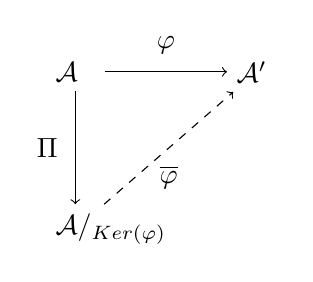
\begin{tikzpicture}
\def \SIZE {2}
\def \MARGINLEFT {5}

\FPeval{\MARGINPLUSSIZE}{\SIZE + \MARGINLEFT}
\FPeval{\MARGINPLUSSIZEPLUSNUMBER}{\MARGINPLUSSIZE + 0.3}
\FPeval{\SIZEHALF}{\SIZE / 2}


\node[text width=0.5cm] (ORIGINAL) at (0,\SIZE) {$\mathcal{A}$};
\node[text width=0.5cm] (QUOTIENT) at (0,0) {$\mathcal{A}/_{Ker(\varphi)}$};
\node[text width=0.5cm] (IMAGE) at (\SIZE.3,\SIZE) {$\mathcal{A}'$};

\draw [->] (ORIGINAL) -- (IMAGE) node [draw=none,midway,above=0.1cm] {$\varphi$};
\draw[->] (ORIGINAL) -- (QUOTIENT) node [draw=none,midway,left=0.1cm] {$\Pi$};
\draw[dashed, ->] (QUOTIENT) -- (IMAGE) node [draw=none,midway,below=0.1cm] {$\overline{\varphi}$};



\end{tikzpicture}
\caption{Komutativni diagram, $\varphi = \overline{\varphi} \circ \Pi$}
\end{figure}
\leavevmode

\begin{remark}
Izrek nam da inducirano preslikavo $\overline{\varphi}$.
%je to vredu izraz?
\end{remark}

\subsection{Zunanji in notranji direktni produkti grup}

Spomnimo se definicije zunanjega produkta grup \ref{def:outer_direct_product_of_groups}. Zunanji produkti nam iz danih grup gradijo nove grupe, medtem ko nam notranji produkti dano grupo (strukturo) razgradijo na "manjše".

\begin{definition}
\label{def:product_subgroup_projection}
Naj bo $\mathcal{G} = \mathcal{G}_1 \times \mathcal{G}_2 \times \dots \times \mathcal{G}_n$ zunanji direktni produkt grup $\mathcal{G}_j$.
\begin{equation}
\label{eq:def_product_subgropu_projection}
\widetilde{\mathcal{G}}_i = \{ (1, \dots , 1, x_i, 1, \dots, 1) | x_i \in \mathcal{G}_i\}
\end{equation}
\end{definition}

Poglejmo si primere za direktni produkt dveh grup.
$\mathcal{G} = \mathcal{G}_1 \times \mathcal{G}_2$\\
$\widetilde{\mathcal{G}}_1 = \{ (x, 1) | x \in \mathcal{G}_1 \}$\\
$\widetilde{\mathcal{G}}_2 = \{ (1, x) | x \in \mathcal{G}_2 \}$\\

\begin{statement}\\
$\mathcal{G}/_{\widetilde{\mathcal{G}}_1} \cong \mathcal{G}_2$
\end{statement}

\begin{proof}
$(x_1, x_2) \mapsto x_2$ je epimorfizem iz $\mathcal{G}$ v $\mathcal{G}_2$, katerega jedro je $\mathcal{G}_1$. Enako velja, če indeksa grup zamenjamo.
\end{proof}

\begin{remark}
S skoraj povsem enakim dokazom zadevo posplošimo na produkt več grup.
\end{remark}

Hitro opazimo naslednje splošne lastnosti grupe $\mathcal{G} = \mathcal{G}_1 \times \mathcal{G}_2 \times \dots \times \mathcal{G}_n$:
\begin{itemize}
\item $\widetilde{\mathcal{G}}_i \triangleleft \mathcal{G} \ \forall i < n$
\item $\mathcal{G} = \widetilde{\mathcal{G}}_1 \widetilde{\mathcal{G}}_2 \dots \widetilde{\mathcal{G}}_n $
\item $\widetilde{\mathcal{G}}_i \cap (\widetilde{\mathcal{G}}_1 \widetilde{\mathcal{G}}_2 \dots \widetilde{\mathcal{G}}_{i-1} \widetilde{\mathcal{G}}_{i+1} \dots \widetilde{\mathcal{G}}_n)  = \{1, 1, \dots, 1, 1\} = \{ 1\} $; za vsak $i$
\end{itemize}

\begin{definition}
\label{def:inner_direct_product}
Grupa $\mathcal{G}$ je \textbf{notranji direktni produkt} svojih edink $\mathcal{N}_1, \mathcal{N}_2, \dots, \mathcal{N}_n$, če velja:
\begin{itemize}
\item $\mathcal{G} = \mathcal{N}_1 \mathcal{N}_2  \dots  \mathcal{N}_n$
\item $\mathcal{N}_i \cap (\mathcal{N}_1 \mathcal{N}_2 \dots \mathcal{N}_{i-1} \mathcal{N}_{i+1} \dots \mathcal{N}_{n}) = \{ 1\}$; za vsak $i$.
\end{itemize}
\end{definition}

\begin{example}
\begin{example_case}
Če je $\mathcal{G}$ zunanji direktni produkt $\mathcal{G}_1, \mathcal{G}_2, \dots ,\mathcal{G}_n$, potem je $\mathcal{G}$ notranji direktni produkt $\widetilde{\mathcal{G}}_1, \widetilde{\mathcal{G}}_2, \dots , \widetilde{\mathcal{G}}_n$.
\end{example_case}
\begin{example_case}
$D_4 = \{ 1, r, z, rz \} $ (komutativna), $\mathcal{N}_1 = \{ 1,r \}, \mathcal{N}_2 = \{1,z\}$. Potem je $D_4$ njun notranji produkt. Spomnimo se, da velja tudi $D_4 \cong \mathbb{Z}_2 \oplus \mathbb{Z}_2$.
\end{example_case}
\begin{example_case}
$\mathcal{G} = \mathbb{C}^{\times}, \mathcal{N}_1 = \mathbb{R}^{+} = \{ r \in \mathbb{R}^{\times} | r > 0\}, \mathcal{N}_2 = \mathbb{S}^{1}$\\
Poljuben $z \in \mathcal{G} = |z| * \frac{z}{|z|}$, prav tako pa velja: $\mathbb{R}^{\times} \cap \mathbb{S}^1 = \{1\}$. $\mathbb{C}^{\times}$ je tako notranji direktni produkt $\mathbb{R}^{+}$ in $\mathbb{S}^1$. Sledi tudi: $\mathbb{C}^{\times}/_{\mathbb{R}^{+}} \cong \mathbb{S}^1$ in $\mathbb{C}^{\times}/_{\mathbb{S}^{1}} \cong \mathbb{R}^+$.
\end{example_case}
\end{example}

\begin{lemma}
Grupa $\mathcal{G}$ je notranji direktni produkt svojih podgrup edink $\mathcal{N}_1, \mathcal{N}_2, \dots \mathcal{N}_n$ natanko tedaj, ko lahko vsak element iz $\mathcal{G}$ na en sam način zapišemo kot produkt $n_1 n_2 \dots n_n$, kjer $n_i \in \mathcal{N}_i$.
\end{lemma}

\begin{proof}\leavevmode\\
$\implies$\\
$\mathcal{G} = \mathcal{N}_1, \mathcal{N}_2 \dots \mathcal{N}_n$. Vsak element lahko na vsaj en način zapišemo kot $n_1 n_2, \dots n_n$. Dokažimo enoličnost:\\
$n_1 n_2 \dots n_n = r_1 r_2 \dots r_n, \ n_i, r_i \in \mathcal{N}_i$. Pomnožimo z leve z $r_1^{-1}$ in z desne z $(n_2 n_3 \dots n_n)^{-1}$\\
$\underbrace{r_1^{-1}n_1}_{\in \mathcal{N}_1} = \underbrace{(r_2 r_3 \dots r_n)(n_2 n_3 \dots n_n)^{-1}}_{\in \mathcal{N}_2 \mathcal{N}_3 \dots \mathcal{N}_n}$ Ker velja $\mathcal{N}_1 \cap (\mathcal{N}_2 \mathcal{N}_3 \dots \mathcal{N}_{n}) = \{1\}$, sledi da $r_1n_1^{-1} = 1$ in torej $r_1 = n_1$. Obe strani enačbe krajšamo in dobimo: $n_2 n_3 \dots n_n = r_2 r_3 \dots r_n, \ n_i, r_i \in \mathcal{N}_i$. Ponavljamo dokler ne pridemo do rezultata, da so vsi členi enaki.\\
$\impliedby$\\
$\mathcal{G} = \mathcal{N}_1, \mathcal{N}_2 \dots \mathcal{N}_n$ sledi iz tega, da obstaja zapis (ne nujno enoličen).\\
$x \in \mathcal{N}_i \cap (\mathcal{N}_1 \mathcal{N}_2 \dots \mathcal{N}_{i-1} \mathcal{N}_{i+1} \dots \mathcal{N}_{n})$, $x = 1 * 1 *\dots n_i * \dots * 1 *1 = n_1 \dots n_{i-1} n_{i+1} \dots n_n$ iz enoličnosti zapisa sledi $n_j = 1$, torej $\mathcal{N}_i \cap (\mathcal{N}_1 \mathcal{N}_2 \dots \mathcal{N}_{i-1} \mathcal{N}_{i+1} \dots \mathcal{N}_{n}) = \{1\}$

\end{proof}

\begin{definition}
\label{def:comutator}
Naj bo $\mathcal{G}$ grupa in $x,y \in \mathcal{G}$. \textbf{Komutator} elementov $x,y$ je:
\begin{equation}
\label{eq:def_comutator}
[x,y] = xyx^{-1}y^{-1}
\end{equation} 
\end{definition}

\begin{remark}
Uporablja se tudi podobna definicija: $[x,y] = x^{-1}y^{-1}xy$.
\end{remark}

\begin{lemma}
Naj bosta $\mathcal{N}, \mathcal{M} \triangleleft \mathcal{G}$. Potem je komutator $[n,m] \in \mathcal{N} \cap \mathcal{M}$ za poljubna $n \in \mathcal{N}, m \in \mathcal{M}$. 
\end{lemma}

\begin{proof}\leavevmode\\
$[n,m] = \underbrace{nmn^{-1}}_{\in \mathcal{M}}m^{-1} \in \mathcal{M}$ in $[n,m] = n\underbrace{mn^{-1}m^{-1}}_{\in \mathcal{N}} \in \mathcal{N}$
\end{proof}

\begin{corollary}
Če je presek $\mathcal{N} \cap \mathcal{M} = \{1\}$ trivialen, potem je $nm=mn, n \in \mathcal{N}, m \in \mathcal{M}$, torej $\mathcal{N}$ in $\mathcal{M}$ med seboj komutirata.
\end{corollary}

\begin{theorem}
Če je grupa $\mathcal{G}$ notranji direktni produkt svojih podgrup edink $\mathcal{N}_1, \mathcal{N}_2 \dots \mathcal{N}_n$, potem je $\mathcal{G}$ izomorfna svojemu zunanjemu direktnemu produktu. Oziroma: $\mathcal{N}_1 \mathcal{N}_2 \dots \mathcal{N}_n \cong \mathcal{N}_1 \times \mathcal{N}_2 \times \dots \times \mathcal{N}_n$.
\end{theorem}

\begin{proof}\leavevmode\\
Definirajmo $\varphi : \mathcal{N}_1 \times \mathcal{N}_2 \times \dots \times \mathcal{N}_n \to \mathcal{G}$, $\varphi( (n_1, n_2, \dots, n_n) ) = n_1 n_2 \dots n_n$\\ Bijektivnost $\varphi$ dobimo iz prejšnje leme o enoličnosti zapisa. Preveriti moramo še, da je tako definirana preslikava res homomorfizem.\\
$\varphi((n_1, n_2, \dots , n_n) (r_1, r_2, \dots r_n)) = n_1r_1 n_2r_2 \dots n_nr_n$. Ali je to enako $n_1n_2 \dots n_n r_1 r_2 \dots, r_n$?
Iz prejšnje leme se spomnimo, da posamezni elementi iz različnih edink med sabo komutirajo (ker imajo po predpostavki trivialen presek), torej enakost velja.

\end{proof}

\begin{remark}
Ker sta si notranji in zunanji produkt po prejšnjem izreku izomorfna, tudi notranji produkt označujemo z $\mathcal{N}_1 \times \mathcal{N}_2 \times \dots \times \mathcal{N}_n$ in pogosto sploh ne ločujemo med notranjim in zunanjim produktom.
\end{remark}

\begin{remark}
Če je $\mathcal{G}$ aditivna grupa, namesto o produkt govorimo o vsoti in pišemo $\mathcal{G} = \mathcal{N}_1 \oplus \mathcal{N}_2 \oplus \dots \oplus \mathcal{N}_n$. Seveda smiselno spremenimo trivialni presek, ki je zdaj $\{0\}$.
\end{remark}

\begin{example}
$\mathcal{N}_1 = \{0,2,4\} \cong \mathbb{Z}_3, \mathcal{N}_2 = \{0,3\} \cong \mathbb{Z}_2$\\ $\mathbb{Z}_6 = \mathcal{N}_1 \oplus \mathcal{N}_2 \cong \mathbb{Z}_3 \oplus \mathbb{Z}_2$, vendar pa $\mathbb{Z}_4 \not \cong \mathbb{Z}_2 \oplus \mathbb{Z}_2$. V $\mathbb{Z}_4$ imamo namreč element reda 4, v $\mathbb{Z}_2$ pa ne (vemo, da bi izomorfizem ohranil red elementa).
\end{example}

\subsection{Direktni produkti in direktne vsote v kolobarjih}
Kolobar $\mathcal{K}$ je med drugim aditivna grupa, zato lahko pišemo $$\mathcal{K} = \mathcal{I}_1 \oplus \mathcal{I}_2 \oplus \dots \oplus \mathcal{I}_n$$ kjer so $\mathcal{I}_j$ poljubne podgrupe za seštevanje. Nas bo bolj zanimal primer, ko so $\mathcal{I}_j$ ideali.

Če je $\mathcal{K} = \mathcal{K}_1 \times \mathcal{K}_2 \times \dots \times \mathcal{K}_n$ direktni produkt kolobarjev $\mathcal{K}_1, \dots , \mathcal{K}_n$, potem je enak direktni vsoti svojih idealov:
$$\mathcal{I}_j = \{(0, \dots , 0, x, 0, \dots, 0) | x \in \mathcal{K}_j\}$$
Da je to res ideal, ni težko pokazati.\\
Radi bi pokazali obratno: če je $\mathcal{K}$ direktna vsota svojih idealov, je $\mathcal{K}$ izomorfen njihovemu direktnemu produktu.

Spomnimo se definicije idempotenta. $e \in \mathcal{K}$ je idempotent, če velja $e^2 = e$. Velja tudi $e^2 = e \iff (1-e)^2 = (1-e)$

\begin{definition}
\label{def:central_idempotent}
Idempotent $e$ kolobarja $\mathcal{K}$ je \textbf{centralni idempotent}, če velja $e \in Z(\mathcal{K})$, torej $ex = xe, \forall x \in \mathcal{K}$. 
\end{definition}

\begin{definition}
\label{def:orthogonal_idempotents}
Idempotenta $e$ in $f$ sta si \textbf{ortogonalna}, če velja $ef = fe = 0$
\end{definition}

\begin{remark}
V tem primeru je idempotent tudi $e+f$
\end{remark}

\begin{definition}
Idempotenti $e_k$ so si paroma ortogonalni, če velja $e_je_i = e_ie_j = 0, j \neq i$.
\end{definition}


\begin{example}
$\mathcal{K} = \mathcal{K}_1 \times \mathcal{K}_2 \times \dots \times \mathcal{K}_n$, $e_j = (0, \dots, 0, 1, 0, \dots ,0)$($1$ na $i$-tem mestu) so si paroma ortogonalni centralni idempotenti z vsoto $1$.
\end{example}


\begin{theorem}
Naj bodo $\mathcal{I}_1, \dots, \mathcal{I}_n$ ideali kolobarja $\mathcal{K}$. Potem velja $\mathcal{K} = \mathcal{I}_1 \oplus \dots \oplus \mathcal{I}_n$ natanko tedaj, ko obstajajo taki paroma ortogonalni idempotenti $e_1, \dots, e_n$, da je njihova vsota $e_1 + \dots + e_n = 1$ in $\mathcal{I}_j = e_j \mathcal{K} := \{ e_j x | x \in \mathcal{K}\}$. 
\end{theorem}

\begin{proof}\leavevmode\\
$\implies$\\
$\mathcal{K} = \mathcal{I}_1 \oplus \dots \oplus \mathcal{I}_n$. Velja $1 = e_1 + e_2 + \dots + e_n$ za neke $e_j \in \mathcal{I}_j$; velja tudi $i \neq j \implies \mathcal{I}_i \mathcal{I}_j \subseteq \mathcal{I}_i \mathcal{I}_j = \{0\}$ in zato $u_i \in \mathcal{I}_i \implies u_i e_j = 0 \implies u_i = u_i*1 = u_i e_i$ in podobno $u_i = e_i u_i$. Posebej $e_i^2 = e_i \in \mathcal{I}_i \implies e_i \mathcal{K} \subseteq \mathcal{I}_i$ in $\mathcal{I}_i \subseteq e_i\mathcal{K}$.\\
Dobimo torej $\mathcal{I}_i = e_i \mathcal{K}$. Iz enakosti prej ($e_iu_i = u_ie_i$) sledi, da so $e_i$ centralni idempotenti.\\
$\impliedby$\\
$x \in \mathcal{K} \implies x = 1x = e_1x + e_2 x + \dots e_n x$. Poglejmo si presek $\mathcal{I}_1 \cap (\mathcal{I}_2 \oplus \dots \oplus \mathcal{I}_n)$. $e_1x = e_2y_2 + \dots + e_n y_n$ za neke $x, y_i \in \mathcal{K}$. Pomnožimo z leve z $e_1$.
$e_1x = e_1e_2y_2 + \dots e_1e_n y_n = 0$, torej je presek ničelen.

\end{proof}

\begin{remark}
Ideali $\mathcal{I}_j = e_j \mathcal{K}$ sicer niso podkolobarji (ker ne vsebujejo enote), so pa sami zase kolobarji s svojo enoto $e_j$.
\end{remark}

\begin{theorem}
Če je kolobar $\mathcal{K}$ direktna vsota svojih idealov, potem je izomorfen direktnemu produktu teh idealov:
$$\mathcal{K} = \mathcal{I}_1 \oplus \mathcal{I}_2 \oplus \dots \oplus \mathcal{I}_n \cong \underbrace{\mathcal{I}_1 \times \mathcal{I}_2 \times \dots \times \mathcal{I}_n}_{\text{Operacija ima smisel v luči opombe, da so ti ideali sami zase kolobarji}}$$
\end{theorem}

\begin{proof} Dokaz bomo zgolj skicirali.
Podobno kot pri enakovrednem izreku za grupe definiramo $\varphi : \mathcal{I}_1 \times \mathcal{I}_2 \times \dots \times \mathcal{I}_n \to \mathcal{I}_1 \oplus \mathcal{I}_2 \oplus \dots \oplus \mathcal{I}_n$, $\varphi( (u_1, u_2, \dots, u_n) ) = u_1 + u_2 + \dots + u_n$.\\
Preverimo, da je $\varphi$ izomorfizem kolobarjev.

\end{proof}

\begin{example}
$(\mathbb{Z}_6, +,*)$ je izomorfen $\mathbb{Z}_3 \times \mathbb{Z}_2$ in enak vsoti idealov $\mathcal{I}_1 = \{0,2,4\}, \mathcal{I}_2 = \{0,3\}; e_1 = 4, e_2 = 3$
\end{example}

\section{Končne grupe}
\subsection{Lagrangeov izrek}

\begin{definition}
\label{def:group_order}
\textbf{Red grupe $\mathcal{G}$} je število njenih elementov.
\begin{equation}
\label{eq:def_group_order}
\ord \mathcal{G} := |\mathcal{G}|
\end{equation}
\end{definition}


\begin{lemma}
Naj bo $\mathcal{H} \leq \mathcal{G}$ in $a \in \mathcal{G}$. Velja: $|a\mathcal{H}| = | \mathcal{H}|$ 
\end{lemma}

\begin{proof}
$f : \mathcal{H} \to a \mathcal{H}, h \mapsto ah$ je očitno bijektivna preslikava
\end{proof}

\begin{definition}
\label{def:subgroup_index}
Naj bo $\mathcal{H}$ podgrupa grupe $\mathcal{G}$. \textbf{Indeks podgrupe $\mathcal{H}$} je moč množice vseh odsekov.
\begin{equation}
\label{eq:def_subgroup_index}
[\mathcal{G}: \mathcal{H}] := | \{a\mathcal{H} | a \in \mathcal{G}\}|
\end{equation}
\end{definition}

\begin{example}
$[\mathbb{Z}: n\mathbb{Z}] = n$
\end{example}
\\\\
\begin{theorem}[Lagrangeov izrek]
\label{th:lagrange_theorem}
Če je $\mathcal{H}$ podgrupa končne grupe $\mathcal{G}$, velja:
\begin{equation}
\label{eq:th_lagrange_theorem}
|\mathcal{G}| = [\mathcal{G}:\mathcal{H}] |\mathcal{H}|
\end{equation}
\end{theorem}

\begin{proof}
Spomnimo se, da je $\mathcal{G}$ disjunktna unija svojih odsekov: $\mathcal{G} = a_1 \mathcal{H} \cup \dots \cup a_r \mathcal{H}$, $r=[\mathcal{G}:\mathcal{H}]$\\
$|\mathcal{G}| = |a_1\mathcal{H}| + |a_2\mathcal{H}| + \dots + |a_r\mathcal{H}| = r|\mathcal{H}| = [\mathcal{G}:\mathcal{H}] |\mathcal{H}|$
\end{proof}

\begin{remark}
Očitno sledi: če $\mathcal{N} \triangleleft \mathcal{G}$, potem $|\mathcal{G}/_{\mathcal{N}}|  = \frac{|\mathcal{G}|}{|\mathcal{N}|}$ (ob predpostavki, da je $\mathcal{G}$ končna).
\end{remark}

\begin{corollary}
Red vsake podgrupe končne grupe deli red grupe.
\end{corollary}

\begin{remark}
Naj bo $\mathcal{G}$ grupa in $a \in \mathcal{G}$, potem veljajo naslednje trditve:
\begin{enumerate}
\item Naj bo $n$ = $\ord a$, potem velja: $a^m = 1 \iff n|m$
\item Če je $p$ praštevilo in je $a^p=1, a \neq 1$, potem velja $p = \ord a$
\item Naj bo $n = \ord a$ in $\varphi : \mathcal{G} \to \mathcal{G}'$ homomorfizem, potem velja $\ord \varphi(a) | \ord a$
\item $\mathcal{N} \triangleleft \mathcal{G} \implies \ord(a\mathcal{N}) | \ord a$
\item $a \in \mathcal{G}, \ord a = \ord <a>$
\end{enumerate} 
\end{remark}

\begin{proof}\leavevmode
\begin{enumerate}
\item $m=kn \implies a^m = (a^n)^k = 1^k = 1$ Obratno: $m = qn +r$, $a^m = a^{qn + r} = a^r = 1 \implies r = 0$ (saj mora biti $r \in \mathbb{N} < n$).
\item Sledi iz prejšnje točke (nobeno drugo število ne deli praštevila).
\item $a^n= 1 \implies \varphi(a)^n = \varphi(a^n) = \varphi(1) = 1$. Po prvi točki torej sledi: če obstaja tak $m < n$, da $\varphi(a)^m = 1$, potem $m |n$. Torej $\ord \varphi(a) | \ord a$.
\item V prejšnjo točko za homomorfizem vstavimo $\Pi$.
\item Podgrupa generirana z $a$ vsebuje elemente $1, a, a^2, \dots, a^{\ord a - 1}$ , torej ravno $\ord a$.
\end{enumerate}
\end{proof}

\begin{corollary}
Red vsakega elementa končne grupe deli red grupe
\end{corollary}

\begin{corollary}
Če je $\mathcal{G}$ končna grupa, za poljuben $a \in \mathcal{G}$ velja $a^{\ord G} = 1$
\end{corollary}

\begin{proof}
Vzemimo $a \in \mathcal{G}$ in naj bo $n = \ord a$, vemo $|\mathcal{G}| = kn$, torej $a^{|\mathcal{G}|} = (a^n)^k = 1^k = 1$
\end{proof}

Poglejmo si še poseben primer: $\mathcal{G} = \mathbb{Z}_p^\times$, kjer je $p$ praštevilo, kot grupo za množenje. Elementi $\mathcal{G}$ so odseki $x + p\mathbb{Z}, x \not \in p \mathbb{Z}$.
Opazimo naslednjo posledico.
\\\\
\begin{theorem}[Mali Fermatov izrek]
\label{th:little_fermat_theroem}
Naj bo $p$ praštevilo in $a \in \mathbb{N}$. Če $p \not | a$, potem $p | a^{p-1} - 1$.
\end{theorem}

\begin{remark}
Ekvivalentna formulacija izreka se glasi: Za poljubno naravno število $a$ in praštevilo $p$ velja: \begin{equation}
\label{eq:th_litttle_fermat_theorem}
a^p \equiv a \Mod p
\end{equation}
\end{remark}

\begin{proof}
$a + p \mathbb{Z} \in \mathbb{Z}_p^\times$
\end{proof}

\begin{corollary}
$(a - p\mathbb{Z})^{p-1} = a^{p-1} + p \mathbb{Z} = 1 + p\mathbb{Z} \iff a^{p-1} - 1 \in p\mathbb{Z}$
\end{corollary}

\begin{corollary}
Vsaka grupa s praštevilskim redom je ciklična (in zato izomorfna $\mathbb{Z}_p$).
\end{corollary}

\begin{proof}
Naj bo $|\mathcal{G}| = p$ praštevilo. \\Izberimo si $a \in \mathcal{G} - \{1 \}$. Potem velja $\{1\} \subsetneq <a> \leq \mathcal{G}$. Od prej vemo $\ord <a> | p \implies \ord <a> = p \implies <a> = \mathcal{G}$
\end{proof}

\begin{remark}
To velja za poljuben $a \neq 1$, torej za vsak $a \neq 1.<a> = \mathcal{G}$. Vidimo, da $\mathcal{G}$ ne vsebuje pravih netrivialnih podgrup (edini podgrupi sta $\{1\}$ in $\mathcal{G}$).
\end{remark}

\begin{corollary}
Grupa $\mathcal{G}$ nima pravih netrivialnih podgrup natanko tedaj, ko je njen red praštevilo.
\end{corollary}

\begin{proof}\leavevmode\\
$\implies$\\
$\mathcal{G}$ nima pravih netrivialnih podgrup. Vzemimo $a \neq 1$ in poglejmo $<a>$. Ker $\mathcal{G}$ nima trivialnih podgrup, velja $<a> = \mathcal{G}$. Torej je $\mathcal{G}$ ciklična in izomorfna $\mathbb{Z}_n$ ali pa $\mathbb{Z}$. Ker $\mathbb{Z}$ vsebuje podgrupe, je torej $\mathcal{G} \cong \mathbb{Z}_n$ za nek $n$. Če $d|n$ in $d \not \in \{1,n\}$, je $d\mathbb{Z}_n$ prava netrivialna podgrupa $\mathbb{Z}_n$, torej je $n$ praštevilo.\\
$\impliedby$ Smo dokazali že v opombi.
\end{proof}

Če je torej moč grupe praštevilo, je taka grupa ciklična. Kaj pa se zgodi, če moč grupe ni praštevilo?\\
$|\mathcal{G}| = 4, \mathcal{G} = \{1,a,b,c\}$\\
Predpostavimo, da $\mathcal{G}$ ni ciklična. Ker je red grupe $4$, imajo lahko elementi $a,b,c$ zgolj red $2$ ali $4$. Če bi bil red kateregakoli izmed njih $4$, bi bila grupa ciklična (generirana s tem elementom). Torej velja $a^2=b^2=c^2 = 1$. Torej $ab \neq 1 \neq a \neq b$. Ostane zgolj še $ab = c$ in podobno za ostale pare. Ugotovimo $\mathcal{G} \cong \mathbb{Z}_2 \oplus \mathbb{Z}_2$.


Poglejmo si nekaj osnovnih grup velikosti $n$
\begin{enumerate}
\item $\{1\}$
\item $\mathbb{Z}_2$
\item $\mathbb{Z}_3$
\item $\mathbb{Z}_4, \mathbb{Z}_1 \oplus \mathbb{Z}_2$(Med seboj si nista izomorfni, sej se red elemento ne ujema)
\item $\mathbb{Z}_5$
\item $\mathbb{Z}_3 \oplus \mathbb{Z}_2, \mathcal{S}_3$
\item $\mathbb{Z}_7$
\item $\mathbb{Z}_8 \underbrace{\mathbb{Z}_4 \oplus \mathbb{Z}_2, \mathbb{Z}_2 \oplus \mathbb{Z}_2 \oplus \mathbb{Z}_2, \mathcal{D}_2, \mathbb{Q}}_{\text{Niso izomorfne} \ \mathbb{Z}_8 \text{, saj so elementi različnih redov}}$
\item $\dots$
\end{enumerate}


Naravno se pojavi vprašanje, kako bi lahko klasificirali končne enostavne grupe. Izkaže se, da si jih da razdeliti na $18$ (neskončnih) družin $(\mathbb{Z}_p, \mathbb{A}_n(n > 5), \dots)$ in $26$ sporadičnih grup (največja med njimi se imenuje "monster" in ima približno $8*10^{53}$ elementov).


\subsection{Razredna formula}
Spomnimo se definicije, kdaj sta si elementa konjugirana(\ref{def:conjugate_elements_group}) in tega, da je to ekvivalenčna relacija.

\begin{definition}
\label{def:conjugate_equivalence_classes}
Grupa $\mathcal{G}$ glede na ekvivalenčno relacijo razpade na ekivalenčne razrede $\mathcal{R}_i$, ki jim pravimo \textbf{konjugirani razredi} in $\mathcal{R}(a)$ označuje ekvivalenčni razred, ki mu pripada $a$.
\begin{equation}
\label{eq:def_conjugate_class}
\mathcal{R}(a) := \{ gag^{-1} | g \in \mathcal{G} \}
\end{equation}
\end{definition}

Ker je $\mathcal{G}$ disjunktna unija svojih ekvivalenčnih razredov lahko zapišemo formulo:
\begin{equation}
\label{eq:power_of_gruop_is_sum_of_conjugate_classes}
|\mathcal{G}| =  \sum |\mathcal{R}_i|
\end{equation}

\begin{definition}
\label{def:centralizatior_of_elment}
\textbf{Centralizator} elementa $a$ grupe $\mathcal{G}$, je grupa vseh elementov, ki z njim komutirajo
\begin{equation}
\label{eq:def_centralizator_of_element}
C(a) := \{ x \in \mathcal{G} | ax = xa \}
\end{equation}
\end{definition}

\begin{lemma}
$C(a)$ je podgrupa $\mathcal{G}$ in velja $|\mathcal{R}(a)| = [\mathcal{G}:C(a)]$
\end{lemma}

\begin{proof}
Vzemimo $x,y \in C(a)$, očitno $xy \in C(a)$, prav tako $ax = xa \implies ax^{-1} = x^{-1}a$ če iz obeh strani pomnožimo z $x^{-1}$.\\
Dokažimo še drug del:\\
$g C(a) = hC(a) \iff h^{-1}g \in C(a) \iff h^{-1}ga = ah^{-1}g \iff gag^{-1} = hah^{-1}$, od tod dobimo da je $gag^{-1} \mapsto gC(a)$ dobro definirana bijekcija iz $\mathcal{R}(a) v \{ gC(a) | g \in \mathcal{G} \}$. \\
\end{proof}

Prav tako sledi $a \in \mathcal{Z}(\mathcal{G}) \iff \mathcal{R}(a) = \{a\} \iff |\mathcal{R}(a)| = 1$.\\
Iz \ref{eq:power_of_gruop_is_sum_of_conjugate_classes} sledi dodatek:
\begin{equation}
|\mathcal{G}| = |Z(\mathcal{G})| + \sum \mathcal{R}_j
\end{equation}
pri čemer so $\mathcal{R}_j$ razredi, ki vsebujejo vsaj dva elementa.

\begin{theorem}
Za vsako končno grupo $\mathcal{G}$ je 
\begin{equation}
|\mathcal{G}| = |Z(\mathcal{G})| + \sum [\mathcal{G}: C(a_j)]
\end{equation}
kjer vsota teče po vseh predstavnikih konjugiranih razredov, ki ne sestojijo iz elementov $Z(\mathcal{G}$
\end{theorem}

\subsection{Cauchiyjev izrek}

NAravno se pojavi vprašanje, če je $\mathcal{G}$ končna grupa, in če $m | \ord \mathcal{G}$, ali potem $\mathcal{G}$ vsebuje element reda $m$? V splošnem, če $\mathcal{G}$ ni ciklična ne vsebuje elementa z redom, ki je enak moči grupe.

\begin{theorem}[Cauchiyjev izrek]
\label{th:cauchy_theroem}
Naj bo $\mathcal{G}$ končna grupa. Če praštevilo $p$ deli $|\mathcal{G}|$, potem $\mathcal{G}$ vsebuje element reda $p$.

\end{theorem}

\begin{proof}
Naj bo $\mathcal{G}$ grupa moči $n= p*k$, pokazali bomo z indukcijo na $n$:
Če je $n = p$, potem je $\mathcal{G}$ ciklična in ima vsak neničelen element red $p$
Če $n > p$, in izrek velja za vse grupe, ki imajo manj kot $n$ elementov:\\
Predpostavimo, da $\mathcal{G}$ ni Abelova in torej $Z(\mathcal{G}) \subsetneq \mathcal{G}$. Če $p | Z(\mathcal{G}$, potem po indukcijski predpostavki obstaja tak element. Torej $p \nmid Z(\mathcal{G})$. Iz razredne formule sledi, da $p \nmid [\mathcal{G}:C(a_j)]$ za nek $a_j \in \mathcal{G}$.
Spet nam preostaneta dve možnosti če $p | |C(a_j)|$ po indukcijsi prespostavki $C(a_j)$ vsebuje element rada $p$. V nasprotnem primeru $p \nmid [\mathcal{G}:C(a_j)]|C(a_j)| = |\mathcal{G}|$ kar pa je v protislovju.\\
Če pa je $\mathcal{G}$ abelova, in ker $n$ ni praštevilo, potem $\mathcal{G}$ kot posledica Lagrangevega izreka vsebuje kako pravo netrivialno podgrupo $\{ 1\} \subsetneq \mathcal{N} \subsetneq \mathcal{G}$ in je $\mathcal{N}$ edinka lahko govorimo o $\mathcal{G}/_{\mathcal{N}}$\\
Če $p | |\mathcal{N}|$, po indukcijski predpostavki imamo tak element, v nasprotnem pa $p \nmid \mathcal{N}$, velja pa $p | \mathcal{G} = |\mathcal{N}| |\mathcal{G}/_{\mathcal{N}}|$ torej $p | |\mathcal{G}/_{\mathcal{N}}$ in ker $\mathcal{N}$ ni trivialna edinka lahko uporabimo predpostavko in dobimo element reda $p$.
\end{proof}
\begin{remark}
Izrek lahko ekvivalentno formuliramo: Če $p$ deli $|\mathcal{G}|$ potem $\mathcal{G}$ vsebuje podgrupi s $p$ elementi. Res, če je $\mathcal{H} = p$ $\mathcal{H} \leq \mathcal{G}$ potem je $\mathcal{H}$ ciklična in vsak njen neničelen element ima red $p$, obratno, če je $a^p = 1 \implies |<a>| = p$.
\end{remark}

Nasploh, ali iz $m| |\mathcal{G}|$ sledi, da $\mathcal{G}$ vsebuje pogrupo z $m$ elementi. V splošnem to ni res($A_n$ ne vsebuje podgrupe s $6$ elementi). Odgovor pa ni pozitiven zgolj za praštevila, ampak tudi za vse njihove potence: $p^k | |\mathcal{G}|$, potem $\mathcal{G}$ vsebuje elemepte reda $p^k$, to pravi prvi izrek Sylowa.


\begin{definition}
Grupa $\mathcal{G}$ se imenuje $p$-grupa, kjer je $p$ praštevilo, če je red vsakega njenega neničelenega elementa potenca števila $p$.
\end{definition}

\begin{example}
$\mathbb{Z}_p, \mathbb{Z}_{p^2}, \mathbb{Z}_{p^3}, \dots$
\end{example}

Direktni produkti $p$-grup so $p$-grupe, prav tako so to njihove podgrupe($\mathcal{D}_4, \mathbb{Q}$)

\begin{corollary}
Končna grupa $\mathcal{G}$ je $p$-grupa natanko tedaj, ko je $|\mathcal{G}| = p^l$ za nek $l \in \mathbb{N}$.
\end{corollary}

\begin{proof}
Če je $\mathcal{G}$ $p$-grupa, potem je po Cauchyjevem izreku $|\mathcal{G}| = p^l$, obratno, $|\mathcal{G}| = p^l \implies $ vsi elementi imajo red $p^k, k \leq l$, po posledici Lagrangevega izreka. 
\end{proof}

\subsection{Končne Abelove grupe}

Tipični primeri končnih Abelovih grup so ciklične grupe $\mathbb{Z}_n$ in njihove direktne vsote.\\
\begin{example}
$\mathbb{Z}_{n_1} \oplus \mathbb{Z}_{n_2} \oplus \dots \mathbb{Z}_{n_r}$
\end{example}

Ali jih imamo še kaj? Ne.\\
$\mathbb{Z}_4 \not \cong \mathbb{Z}_2 \oplus \mathbb{Z}_2, \mathbb{Z}_6 \cong \mathbb{Z}_3 \oplus \mathbb{Z}_2$

Po dogovoru bodo grupe v tem razdelku aditivne, im bom operacijo pisali kot $+$.

\begin{lemma}
Demimo, da je $|\mathcal{G}| = mn$ in sta si $m$ in $n$ tuji števili. potem je $\mathcal{G}$ direktna vsota svojih podgrup $\mathcal{H} = \{x \in \mathcal{G} | mx = n\}, \mathcal{K} = \{ x \in \mathcal{G} | nx = 0\}$
\end{lemma}

\begin{proof}
Očitno sta $\mathcal{H}, \mathcal{K} \leq \mathcal{G}$\\
$x^{|\mathcal{G}|} = 1 \forall x \in \mathcal{G} \implies x^{mn} = 0 \forall x \in \mathcal{G}$, torej je $nx \in \mathcal{H}$ in $mx \in \mathcal{K}$, ker sta si tuji, $\exists u,v \in \mathbb{Z}. um + vn = 1$ in $u\underbrace{(mx)}_{\in \mathcal{K}} + v\underbrace{(nx)}_{\in \mathcal{H}} = x \implies \mathcal{G} = \mathcal{H} + \mathcal{K}$, preverimo, še da je presek ničelen $x \in \mathcal{H} \cap \mathcal{K} \implies mx = nx = 0 \implies x = 0$
\end{proof}

Tako lahko posplošimo: $\mathbb{Z}_mn \cong \mathbb{Z}_m \oplus \mathbb{Z}_n$, kjer sta si $m$ in $n$ tuji števili.




\begin{lemma}
Naj bo $\mathcal{G}$ grupa in naj velja $|\mathcal{G}| = p_1^{k_1}p_2^{k_2} \dots p_n^{k_n}$, kjer so $p_i$ različna praštevila, potem je 
$$ \mathcal{G} = \mathcal{H}_1 \oplus \mathcal{H}_2 \oplus \dots \oplus \mathcal{H}_n$$
kjer so $\mathcal{H}_i$ $p_i-$ grupe in velja $|\mathcal{H}_i| = p_i^{k_i}$
\end{lemma}

\begin{proof}
Definirajmo: $\mathcal{H}_1 := \{ x \in \mathcal{G} | xp_1^{k_1} = 0\}$ in \\
$\mathcal{K} =  \{ x \in \mathcal{G} | p_2^{k_2} \dots p_n^{k_n} \}$\\
Vemo, da $p_1 \nmid | \mathcal{K}|$, saj bi sicer po Cauchyjevem izreku $\mathcal{K}$ vsebovala element reda $p$ in bi zato veljalo $p_1 | p_2^{k_2} \dots p_n^{k_n}$, kar pa je protislovje.
Tako je edina možnost $|\mathcal{G}| = |\mathcal{H}_1| |\mathcal{K}| = p_1 * p_2^{k_2} \dots p_n^{k_n}$
\end{proof}

\begin{lemma}
Naj go $\mathcal{G}$ $p-$grupa. Potem je $\mathcal{G}$ ciklična natanko tedaj, ko vsebuje eno samo podgrupo reda $p$.
\end{lemma}

\begin{remark}
Vsaka $p-$grupa vsebuje kako podgrupo reda $p$ (Po Cauchyjevem izreku), če pa ni siklična pa vsaj $2$.
\end{remark}

\begin{proof}\leavevmode\\
$\implies$Ker je $\mathcal{G}$ ciklična velja $\mathcal{G} \cong \mathbb{Z}_{p^m}$, kot vemo pa so edine pogrupe $\mathcal{G}$ grupe oblike: $p^i \mathbb{Z}_{p^k}$, kjer ima samo $p^{m-1}\mathbb{Z}_{p^m}$ $p$ elementov.


$\impliedby$ Naj ima $\mathcal{G}$ natanko eno podgrupo reda $p$, imenujmo jo $\mathcal{N}$. Imamo dve možnosti, če $|\mathcal{G}| = p$, potem velja $\mathcal{G} = \mathcal{N}$ in $\mathcal{G}$ je ciklična. drugače pa velja $|\mathcal{G}| > p$ in predpostavimo, da lema velja za vse grupe, ki imajo manj elementov, kot grupe $\mathcal{G}$.\\
Vpeljimo $\varphi: \mathcal{G} \to \mathcal{G}, \varphi(x) = px$, ki je endomorfizem, katerega jedro sestoji iz elementov z redom $p$. Zato velja $Ker (\varphi) = \mathcal{N}$. Po izreku o izomorfizmih tako velja: $\mathcal{G}/_{\mathcal{N}} \cong Im(\varphi) \leq \mathcal{G}$ in $|Im(\varphi)| = \frac{|\mathcal{G}|}{|\mathcal{N}|} \leq \mathcal{G}$. Tako lema po predpostavki velja za grupo $Im(\varphi)$.\\
Kot prodgrupa $Im(\varphi)$ ne more vsebovati več podgrup reda $p $ kot $\mathcal{G}$, zato vsebuje eno samo in je torej ciklična. zato je tudi $\mathcal{G}/_{\mathcal{N}}$ ciklična z generatorjem $a + \mathcal{N}$, iz tega sledi: $\mathcal{G} = <a> + \mathcal{N}$. Tako dobimo $|\mathcal{G}| > p = |\mathcal{N}|$ in zato je $<a>$ netrivialna podgrupa $\mathcal{G}$ in po Cauchyjevem izreku zato vsebuje element reda $p$. Sledi $\mathcal{N} \subseteq <a>$ in zato $\mathcal{G} = <a>$.
\end{proof}

Spomnimo se vektroskih prostorov. Če je $\mathcal{U}$ vektorski podprostor $\mathcal{V}$, potem obsjata podprostor $\mathcal{W}$, da velja $\mathcal{V} = \mathcal{U} \oplus \mathcal{W}$. Za grupe ne velja nič podobnega. Grupa $\mathbb{Z}_4$ in podgrupa $\{0,2\}$ nimata komplementa da velja $\mathbb{Z}_4 = \{0,2\} \oplus \mathcal{G}$.

\begin{lemma}
Naj bo $\mathcal{G}$ $p-$grupa. Če je $\mathcal{C}$ njena ciklična podgrupa, ki ima izmed vseh cikličnih podgrup največji red, potem $\mathcal{G}$ vsebuje tako podgrupo $\mathcal{K}$, da velja: $\mathcal{G} = \mathcal{V} \oplus \mathcal{K}$.
\end{lemma}

\begin{proof}
Če je $\mathcal{G}$ ciklična, potem $\mathcal{G} = \mathcal{C}$ in $\mathcal{K} = \{0\}$, torej smemo privzeti, da $\mathcal{G}$ ni ciklična, $|\mathcal{G}| > p$ in da lema velja za vse grupe z manj elementi kot $p$.\\
Ker po lemi vemo, da če $\mathcal{G}$ ni ciklična ima vsaj dve podgrupi reda $p$, $\mathcal{C}$ pa zgolj eno samo. Naj bo $\mathcal{N}$ podgrupa reda $p$, ki ni vsebovana v $\mathcal{C}$. Dobimo $\mathcal{C} \cap \mathcal{N} = \{0\}$ saj je presek podgrupa grupe $\mathcal{N}$ in ima zato $p^j$ elementov ($j = 0$). Tako velja $\mathcal{C} + \mathcal{N} = \mathcal{C} \oplus \mathcal{N}$ in $\mathcal{C} + \mathcal{N}/_{\mathcal{N}} \cong \mathcal{C}$ ($c \mapsto c + \mathcal{N}$) in tako dobimo: $(\mathcal{C} + \mathcal{N})/_{\mathcal{N}} \cong \mathcal{C}$.\\
v $\mathcal{G}/_{\mathcal{N}}$ tako ni cikličnih podgrup z več elemnti kot jih ima $\mathcal{C}$ (saj je red elemeta $x+ \mathcal{N} \in \mathcal{G}/_{\mathcal{N}}$ kvečjemu manjši kot red elementa $x$. Zato ima $(\mathcal{C} + \mathcal{N})/_{\mathcal{N}}$ izmed vseh cikličnih pogrup grupe $\mathcal{G}/_{\mathcal{N}}$ največji red $|\mathcal{G}/_{\mathcal{N}}| < \mathcal{G}$ in tako po naši predpostavki velja $\mathcal{G}/_{\mathcal{N}} = (\mathcal{C} + \mathcal{N})/_{\mathcal{N}} \oplus \mathcal{L}$ za neko podgrupo $\mathcal{L} \leq \mathcal{G}/_{\mathcal{N}}$.\\
Po znane izreku je tako res: $\mathcal{L} = \mathcal{K}/_{\mathcal{N}}, \mathcal{N} \leq \mathcal{K} \leq \mathcal{G}$, potrebno je še dokazati: $\mathcal{G} = \mathcal{V} \oplus \mathcal{K}$. Vemo: $\mathcal{G}/_{\mathcal{N}} = ((\mathcal{C} + \mathcal{N})/_{\mathcal{N}}) \oplus (\mathcal{K}/_{\mathcal{N}} \implies \mathcal{G} = \mathcal{C} + \mathcal{N} + \mathcal{K}$ in potrebujemo zgolj še $\mathcal{C} \cap \mathcal{K} = \{0\}$.\\
Vzemimo $x \neq 0$ iz preseka. $x \notin \mathcal{N} \implies x + \mathcal{N}$ je neničelen element $(\mathcal{C} + \mathcal{N})/_{\mathcal{N}} \cap \mathcal{K}/_{\mathcal{N}}$, kar pa je protislovje.

\end{proof}

\begin{theorem}[Osnovni izrek o končnih Abelovh grupah]
\label{th:fundamental_theorem_of_finite_abel_group}
Vsaka končna Abelova grupa je direktna vsota cikličnih podgrup. Te podgrupe lahko izberemo tako, da je red vsake izmed njih potenca praštevil.
\end{theorem}

\begin{proof}
Po predzadnji lemi zadošča obravnavati zgolj situacijo, ko je $\mathcal{G}$ $p-$grupa in tako po zadnji lemi dobimo $\mathcal{G} = \mathcal{C} \oplus \mathcal{K}$, $|\mathcal{C}| \geq p$ in $\mathcal{G}$ ciklična, potem $|\mathcal{K}| < |\mathcal{G}|$. Uporabimo zadnjo lemo za $\mathcal{K}$ in po končnem številu korakov dobimo željeno.
\end{proof}

\begin{remark}
Krajše lahko zadevo zapišemo: $\mathcal{G}$ je (notranja) direktna vsota cikličnih $p$ podgrup. Ali ekvivalentno: $\mathcal{G}$ je izomorfna (zunanji) direktni vsoti grup  oblike $\mathbb{Z}_{p^i}$, kjer je $p$ praštevilo.
\end{remark}

Naravno nas zanima, katere izmed teh grup so si med seboj izomorfne.

Naj bosta $\mathcal{G}$ in $\mathcal{G}'$ končni Abelovi grupi: $\mathcal{G} \cong \mathcal{G}'$, $|\mathcal{G}| = |\mathcal{G}'| \implies \mathcal{G} = \mathcal{H}_1 \oplus \dots \oplus \mathcal{H}_s, \mathcal{G}' = \mathcal{H}_1' \oplus \dots \mathcal{H}_s'$, kjer sta $\mathcal{H}_i, \mathcal{H}_i'$ $p_i-$grupi.\\
Izomorfizem $\varphi \mathcal{G} \to \mathcal{G}'$ pa slika eno v drugo. Zato je potrebno odgovoriti le za $p-$grupe.\\
$\mathcal{G}$ je $p-$grupa $\implies \mathcal{G} \cong \mathbb{Z}_{p^{k_1}} \oplus \dots \oplus \mathbb{Z}_{p^{k_n}}$, brez škode za splošnost pa lahko privzamemo $k_1 < \geq k_2 \geq \dots \geq k_n$
\\\\
\begin{theorem}
Naj bo $p$ preštevilo. Če za naravna števila $k_1 \geq k_2 \geq \dots \geq k_u$ in $l_1  \geq l_2 \geq \dots \geq l_v$ velja $\mathbb{Z}_{p^{k_1}} \oplus \dots \oplus \mathbb{Z}_{p^{k_u}} \cong \mathbb{Z}_{p^{l_1}} \oplus \dots \oplus \mathbb{Z}_{p^{l_v}}$ potem je $k_i = l_i$ in $u = v$.
\end{theorem} 

\begin{proof}
Seveda se vsoti ujemata in sta enaki moči grup. Naj bo $|\mathcal{G}| > p$ in privzemimo, da izrek velja za grupe z manj elementi kot $\mathcal{G}$. Za nako poljubno podgrupo $\mathcal{K}$ pišimo $p\mathcal{K} := \{ px | x \in \mathcal{K} \}$. Tako dobimo $p \mathbb{Z}_{p^m} \cong \mathbb{Z}_{p^{m-1}} (m=1: p\mathbb{Z}_p = \{0\}$ in $\mathcal{G} \cong \mathcal{G}' \implies p\mathcal{G} \cong p\mathcal{G}' \implies \mathbb{Z}_{p^{k_1 - 1}} \oplus \dots \oplus \mathbb{Z}_{p^{k_w - 1}} \cong \mathbb{Z}_{p^{l_1 - 1}} \oplus \dots \oplus \mathbb{Z}_{p^{l_z - 1}}$, kjer je $w$ največji indeks $k_w > 1$ in $z$ največji indeks $k_z > 1$. Po predpsotavki tako dobimo $w = z$ in $k_i - 1 = l_i - 1$, ker pa $k_1 + \dots + k_w - w = l_1 + \dots + l_w - w$ in imata grupi enako moč dobmio $u = v$.

\end{proof}

\begin{example}
$|\mathcal{G}|$ je Abelova in $|\mathcal{G}| = 200 = 5^2*2^3$, $\mathcal{G} = \mathcal{H} \oplus \mathcal{K}$, $|\mathcal{H}| = 25$ in $|\mathcal{K}| = 8$.\\
Za $\mathcal{H}$ imamo (do izomorfizma natančno) dve možnosti: $\mathbb{Z}_25$ ali $\mathbb{Z}_5 \oplus \mathbb{Z}_5$, za $\mathcal{K}$ pa $\mathbb{Z}_8$ ali $\mathbb{Z}_2 \oplus \mathbb{Z}_4$ ali $\mathbb{Z}_2 \oplus \mathbb{Z}_2 \oplus \mathbb{Z}_2$. Torej je $\mathcal{G}$ izomorfna eni izmed grup, ki o dobimo s kombinacijo prve ali druge možnosti.
\end{example}

\begin{remark}
Osnovni izrek za \textbf{končno generirane} Abelove grupe: Vsaka taka grupa je izomorfna $\mathbb{Z}^m\oplus \mathcal{K}$, kjer je $\mathcal{K}$ končna Abelova grupa. Tako je vsaka taka grupa direktna vsota cikličnih grup.
\end{remark}

\section{Deljivost v komutativnih kolobarjih}
\subsection{Glavni ideal}

\begin{definition}
\label{def:main_ideal}
Naj bo $\mathcal{K}$ komutativen kolobar in $a \in \mathcal{K}$. Množica
\begin{equation}
\label{eq:def_main_ideal}
(a) := \{ ax | x \in \mathcal{K} \}
\end{equation}
je \textbf{ideal generiran z $a$}.
\end{definition}

\begin{definition}
Ideal kolobarja je glavni ideal, če je generiran z enim samim elementom.
\end{definition}

\begin{remark}
Če $\mathcal{K}$ ni komutativen kolobar je 
$$(a) := \{\sum_i x_iay_i \ | \ x_i, y_i \in \mathcal{K} \} $$ 
\end{remark}

\begin{example}
$\mathcal{K} = \{1\}$ in $(0) = \{0\}$
\end{example}

\begin{statement}
$\mathcal{K} = (a)$ natanko tedaj, ko je $a$ obrnljiv.
\end{statement}

\begin{proof}\leavevmode\\
$\implies$ Enačba $ax = 1$ ima rešitev, torej je $a$ obrnljiv \\
$\impliedby$ Vemo od prej

\end{proof}

\begin{example}
$\mathcal{K} = \mathbb{Z}$, vsi ideali so oblike $n\mathbb{Z}, n \geq 0$ in zato so vsi glavni.
\end{example}

\begin{definition}
Ideal je \textbf{končno generiran}, če je generiran s končno mnogo množico elementov. Oznalimo ga z $(a_1, a_2, \dots, a_n)$
\end{definition}

\begin{remark}
Opazimo, da velja $(a_1, a_2, \dots, a_n) = (a_1) + (a_2) + \dots + (a_n)$ in torej $(a_1, a_2, \dots, a_n) = \{ a_1x_1 + a_2x_2 + \dots + a_nx_n \ | \ x_i \in \mathcal{K} \}$
\end{remark}

\begin{example}
\begin{example_case}
$(4,6)\triangleleft \mathbb{Z}$ $(4,6) = \{ 4x + 6y \ | \ x,y \in \mathbb{Z} \} = (2)$, torej lahko generatorja $4,6$ nadomestimo z enim samim $2$.
\end{example_case}
\begin{example_case}
Naj bo $\mathcal{F}$ polje in naj bo $\mathcal{I}$ množica vseh polinomov iz $\mathcal{F}[X]$ s konstantnim členom $0$. Velja $\mathcal{I} = (X)$. Kasneje bomo pokazali, da so vsi ideali $\mathcal{F}[X]$ glavni.
\end{example_case}
\begin{example_case}
$\mathbb{Z}[X]$ ($\mathbb{Z}$ ni polje), $(2,X)$ sestoji iz polinomov, ki imajo konstanten člen sod. Ta ideal pa ni glavni, saj če bi veljalo: $(2,X) = (f(X))$, cin $2 \in (f(X))$, sledi, da je $f(X)$ konstanten polinom $a_0$, ki je sod, kar pa je v protislovju s predpostavko da $X \in (a_0)$
\end{example_case}
\begin{example_case}
$\mathcal{F}[X,Y]$, $\mathcal{I}$ vsebuje vse polinome s konstantim členom $0$, torej $\mathcal{I} = (X,Y)$, bralec pa bo za domačo nalogo lahko preveril, da $\mathcal{I}$ ni glavni ideal.
\end{example_case}
\end{example}

\subsection{Deljivost}

\begin{definition}
\label{def:divides_ring}
Naj bo $\mathcal{K}$ komutativen kolobar. Neničelen element $b$ \textbf{deli} element $a$, če obstaja  tak $q \in \mathcal{K}$, da velja $a = bq$. V tem primeru rečemo, da je $a$ deljiv z $b$.
\begin{equation}
\label{eq:def_divides_ring}
b \mid a \iff \exists q \in \mathcal{K}. \ a = bq 
\end{equation}
\end{definition}


\begin{statement}
$$b \mid a \iff (a) \subseteq (b)$$
\end{statement}

\begin{proof}\leavevmode \\
$\implies$ \\
$b \mid a \implies a = bq \implies (a) \subseteq (b)$
\\$\impliedby$\\
$(a) \subseteq (b) \implies a \in (b) \implies a = bq$
\end{proof}

\begin{remark}
V posebnem primeru dobimo: $$b \mid a \land a \mid b \iff (a) = (b)$$
\end{remark}

\begin{definition}
V primeru, da $a \mid b$ in $b \mid a$ pravimo, da sta si $a$ in $b$ \textbf{asociirana}.
\end{definition}

\begin{statement}
Naj bo $\mathcal{K}$ cel kolobar (torej komutativen in brez deliteljev niča), potem sta si neničelna elementa $a$ in $b$ asiciiriana natanko tedaj, ko obstaja tak obrnljiv elementa $u \in \mathcal{K}$, da velja $a = ub$.
\end{statement}

\begin{proof}\leavevmode\\
$\implies$\\
$a \mid b \land b \mid a, a,b \neq 0$\\
$b = ar, a = bq \implies b = ar = (bq)r = b(qr) \implies b(1-qr) = 0$, ker pa $b \neq 0$, sta $q, r$ obrnljiva.\\
$\impliedby$\\
Zgolj premečemo definicjo.

\end{proof}

\begin{example}
\begin{example_case}
V $\mathbb{Z}$ sta si števili asociirani natanko tedaj, ko sta si enaki ali ko velja $n = -m$, saj sta $1$ in $-1$ edina obrnljiva elementa.
\end{example_case}
\begin{example_case}
Obrnljivi elementi v $\mathcal{F}[X]$ so neničelni konstanti polinomi, $f(x) in g(x)$ sta si asociirana $\iff$ $f(X) = ug(X)$ za nek $u \in \mathcal{F} \neq 0$  
\end{example_case}
\end{example}

\begin{remark}
Iz definicij sledi, da asociirana elementa delite iste elemente in sta z istimi elementi deljiva. S stališča teorije deljivosti ju zato lahko identificiramo.
\end{remark}

\begin{definition}
\label{def:gcd_ring}
Naj bo $\mathcal{K}$ komutativen kolobar in $a,b \in \mathcal{K}$ neničelna. Neničelni $d \in \mathcal{K}$ je njun \textbf{največji skupni delitelj}, če velja:
\begin{itemize}
\item $d \mid a \land d \mid b$
\item $c \mid a \land c \mid b \implies c \mid d$
\end{itemize}
Pišemo $\gcd(a,b) = d$
\end{definition}

\begin{remark}
Največji skupni delitelj števil ne obstaja vedno, če pa obstaja, potem je določen do asociiranosti natančno.
\end{remark}

\begin{remark}
Po dogovoru v $\mathbb{Z}$ za $\gcd$ izberemo naravno število in je tako $\gcd$ natančno določen. Podobno v $\mathcal{F}[X]$ za $\gcd$ izberemo polinom, ki ima vodilni koeficient $1$.
\end{remark}

\begin{definition}
Elementa $a$ in $b$ sta si \textbf{tuja}, če velja $gcd(a,b) = 1$
\end{definition}


\begin{statement}
Naj bo $\mathcal{K}$ komutativen in $a,b \in \mathcal{K}$ ne oba enaka $0$, če je idal $(a,b)$ glavni, potem $\gcd(a,b)$ obstaja in je oblike $d = ax + by$ za neka $x,y \in \mathcal{K}$.
\end{statement}

\begin{proof}
Po predpostavki je $(a,b) = (d)$ za nek $d \neq 0 \in \mathcal{K}$, vemo $a \in (d) \implies d \mid a, b \in d \implies d \mid b$\\
$d \in (d) = (a,b) \implies d =ax + by$\\
 $c \mid a, c \mid d$, $a = cz, b= cw \implies d = c(zx +wy) \implies c \mid d$
\end{proof}

\begin{remark}
Četudi ideal $(a,b)$ ni glavni ideal lahko njun $\gcd$ še vedno obstaja. V $\mathbb{Z}[X]$ je tako $\gcd(2, X) = 1$. 
\end{remark}

\begin{definition}
Naj bo $\mathcal{K}$ komutativen. Neničelen $p \in \mathcal{K}$, ki ni obrnljiv je \textbf{nerazcepen}, če iz $p = ab$ sledi, da je (vsaj) eden izmed elementov $a,b$ obrnljiv.
\end{definition}

\begin{example}
V $\mathbb{Z}$ so nerazcepni elementi $p, -p$, kjer je $p$ praštevilo.
\end{example}

\begin{statement}
Naj bo $\mathcal{K}$ cel kolobar in $p \in \mathcal{K}$, tedaj sta za neničelen in neobrnljiv $p$ naslednji trditvi ekvivalentni:
\begin{itemize}
\item $p$ je nerazcepen
\item Če je $a \in \mathcal{K}$ tak, da $(p) \subseteq (a)$ in $(a) \neq \mathcal{K}$, potem $(p) = (a)$
\end{itemize}
\end{statement}

\begin{proof}
$(p) \subseteq (a)$ pomeni $p = ab$ za nek $b$. $(a) \neq \mathcal{K}$ pomeni, da $a$ ni obrnljiv, $(p) = (a)$ pa, da sta si $p$ in $a$ asociirana ($ua = p$ za nek obrnljiv $u$)\\
$p = ab = ua \implies b=u$ in sledi, da sta si trditvi ekvivalentni.

\end{proof}

\subsection{Evklidski kolobarji}

Če si podrobneje pogledamo, vidimo da sta si $\mathbb{Z}$ in $\mathcal{F}[X]$ zelo podobna, oba sta cela in imata zelo "malo" obrnljivih elementov. Oba zadoščata osnovnemu izreku o deljenju (\ref{th:fundamental_theorem_of_division}).
 

\begin{theorem}[Osnovni izrek o deljenju polinomov]
\label{def:fundamental_theorem_of_polynomial_division}
Naj bo $\mathcal{F}$ polje in naj bosta $f(X), g(X) \in \mathcal{F}[X]$, Če $g(X) \neq 0$ potem obstajata taka $q(X), r(X) \in \mathcal{F}[X]$, da velja 
\begin{equation}
\label{eq:def_fundemantal_theorem_of_polynomial_division}
f(X)= q(X)g(X) + r(X), r(X) = \lor st(r(X)) < st(g(X))
\end{equation} 
\end{theorem}

\begin{proof}
$n := st(g(X)), m := st(f(X))$, $m < n \implies q(X) = 0, r(X) = f(X)$, torej naj bo $m \geq n$, izrek pa bomo dokazali z indukcijo na $m$.\\
$m = 0 \implies n = 0$ in trivialno dobimo $r(X) = 0$\\
$f(X) = aX^n + f_1(X), st(f_1(X)) < m$. $g(X) = bX^n + g_1(X)$, $st(g_1(X)) < n$\\
$h(X) := f(X)- ab^{-1}X^{m-n}g(X) = \underbrace{f_1(X) - ab^{-1}X^{m-n}g_1(X)}_{\text{stopnja } \ < m}$\\
Po indukcijski predpostavki velja $h(X) = q_1(X)g(X) + r(X), r=0 \lor st(r(X)) < n$
$f(X) - ab^{-1}X^{m-n}g(X) = q_1(X)g(X) + r(X) \implies$\\ $f(X) = \underbrace{(ab^{-1}X^{m-n} + q_1(X))}_{q(X)}g(X) + r(X)$
\end{proof}


\begin{definition}
\label{def:euclidean_ring}
Cel kolobar $\mathcal{K}$ je \textbf{evklidksi kolobar} če obstaja taka preslikava $\sigma : \mathcal{K} - \{0\} \to \mathbb{N} \cup \{0\}$, za katero velja:
\begin{itemize}
\item $\forall a,b \in \mathcal{K}, b \neq 0. \exists q,r \in \mathcal{K}. \ a= qb +r, r = 0 \lor \sigma(r) < \sigma(b)$ (izrek o deljenju)
\item $\forall a,b \in \mathcal{K}- \{0\}. \ \sigma(a) \leq \sigma(ab)$
\end{itemize} 
\end{definition}

\begin{example}
\begin{example_case}
$\mathbb{Z}, \sigma(n) = |n|$
\end{example_case}
\begin{example_case}
$\mathcal{F}[X], \sigma(f(X)) = st(f(X))$
\end{example_case}
\begin{example_case}
$\mathbb{Z}[i]$ je evklidski za $\sigma(n+mi) = n^2 + m^2$
\end{example_case}
\begin{example_case}
$\mathcal{F}$ je evklidski, saj je zaradi deljenja vedno: $r=0$, tako je lahko $\sigma$ poljubna funkcija, ki ustreza drugemu pogoju.
\end{example_case}
\end{example}

\begin{statement}
$\sigma(a) = \sigma(ab) \implies b$ je obrnljiv
\end{statement}

\begin{proof}
$a = qab + r, r= 0 \lor \sigma(r) < \sigma(ab)$. \\
Če $r = 0 \implies a(1-qb) = 0  \underbrace{\implies}_{a \neq 0} b = q^{-1}$\\
Če $r \neq 0 \implies r = a(q-qb)$ in zato $\sigma(r) \geq(a)$, kar pa je protislovje.
\end{proof}

\begin{remark}
$\sigma(u) = 0 \implies u$ je obrnljiv. $1 = qu + r \implies r = 0$
\end{remark}

\begin{theorem}
Vsak ideal evklidskega kolobarja je glavni.
\end{theorem}


\begin{proof}
Naj bo $\mathcal{I} \triangleleft \mathcal{K}$, kjer je $\mathcal{K}$ evklidski. Izberimo si $a \in \mathcal{I} - \{0\}$, da zanj velja $\sigma(a) \leq \sigma(x), x \in \mathcal{I}$ (to lahko naredimo, saj za naravna števila velja načelo dobre urejenosti. Pokazali bomo da velja $\mathcal{I} = (a)$, vemo že da $(a) \subseteq \mathcal{I}$. Vemo tudi $x \in \mathcal{I}. x = qa +r$ Če $r = 0: x = qa \in (a)$, Če pa $\sigma(r) < \sigma(a), r = x- qa \in \mathcal{I}$, kar pa je protislovje.
\end{proof}


\begin{corollary}
Naj bo $\mathcal{K}$ evklidksi kolobar in $p \in \mathcal{K}, p \neq 0$, naslednje trditve so si ekvivalentne:
\begin{enumerate}
\item $p$ je nerazcepen
\item $(p)$ je maksimalen ideal
\item $\mathcal{K}/_{(p)}$ je polje
\end{enumerate} 
\end{corollary}

\begin{proof}
$(1) \iff (2)$, v prejšnjem razdelku smo dokazali, da je nerazcepnost ekvivalentena maksimalnosti.\\
$(2) \iff (3)$ Smo dokazali v poglavju $4$.
\end{proof}

\begin{example}
Za $\mathbb{Z}$ to že poznamo ($p$ je praštevilo $\iff \mathbb{Z}/_{p\mathbb{Z}} = \mathbb{Z}_p$ je polje 
\end{example}

\begin{corollary} %posledica posledice............
Naj bo $\mathcal{K}$ evklidski kolobar. Za vsaka $a,b \in \mathcal{K}$, ki nista oba $0$ velja, da obstaja njun $\gcd$, ki je oblike $\gcd(a,b) = ax + by; \ x,y \in \mathcal{K}$
\end{corollary}

\begin{proof}
Že prej smo dokazali, da je vsak tak kolobar glavni in da temu ustreza.
\end{proof}

\begin{corollary}
Naj bo $\mathcal{K}$ evklidski kolobar in $a,b, p \in \mathcal{K}$. Če je $p$ nerazcepen in $p \mid ab$, potem $p \mid a \lor p \mid b$.
\end{corollary}

\begin{proof}
Denimo, da $p \nmid a$, potem sta si $p$ in $a$ tuja, zato po prejšnji posledici velja $ax + py = 1$ za nkea $x,y \in \mathcal{K}$\\
$abx = bpy = y \implies p(cx+by) = b \implies p\mid b$
\end{proof}

\begin{remark} %mogoce definicija
Fraza \textbf{enoličnost do vrstnega reda asociiranosti} pomeni $a= p_1p_2 \dots p_s = q_1 q_2\dots q_t$, ker so $p_i, q_i$ nerazcepni pomeni, da ob pogoju $s = t$ obstaja permutacija $\sigma \in \mathcal{S}_s$, da velja $p_i$ je asociiran $q_{\sigma(i)}$. 
\end{remark}


\begin{theorem}
\label{th:unique_factorization_in_ring}
Naj bo $\mathcal{K}$ evklidski kolobar, vsak neničelni $a \in \mathcal{K}$, ki ni obrnljiv lahko zapišemo kot produkt nerazcepnih elementov. Ta zapis je enoličen do vrstnega reda in asociiranosti faktorjev natančno.
\end{theorem}

\begin{proof}
$a \in \mathcal{K}, a \neq 0$, a ni obrnljiv. Predpostavimo, da $a$ ni nerazcepen, torej $a = a_1a_2$, kjer sta $a_1$ in $a_2$ obrnljiva, velja tudi $\sigma(a_1) < \sigma(a), \sigma(a_2) < \sigma(a)$ tako nadaljujemo za navzdol, doker ne pridemo do $a$ja, kjer velja $\sigma(a) = 0$.\\
Potrebno je dokazati še enoličnost.
$a = p_1 p_2 \dots p_s = q_1 q_2 \dots q_t$, kjer so $p_i, q_i$ nerazcepni, po posledici pa $p_1 \mid p_i$ za nek $i$. $q$-je permutiramo, in $p_1 \mid q_1$ in $q_1 = p_1 u$, kjer je $u$ obrnljiv. $p_1$ in $q_1$ sta si asociirana. Krajšamo s $p_1$ in dobimo $p_2 \dots p_s = (uq_2)\dots q_t$, kjer je $uq_2$ nerazcepen. Postopek ponavljamo dokler ne končamo.
\end{proof}

\begin{remark}
Vse posledice zadnjega izreka veljajo tudi za \textbf{glavne kolobarje} (celi kolobarji, v katerih je vsak ideal glaven), venad se je za dokaz potrebno nekoliko bolj potruditi.
\end{remark}

\begin{remark}
Vsak evklidski kolobar je glavni, obratno pa v splošnem ne velja.
\end{remark}

\begin{definition}
\textbf{Kolobar z enolično faktorizacijo} je cel komutativen kolobar, za katerega velja izrek (\ref{th:unique_factorization_in_ring}).
\end{definition}


\begin{definition}
\textbf{Noetherski kolobar} je komutativen kolobar, v katerem je vsak ideal končno generiran.
\end{definition}


\begin{remark}
Izkaže se:\\
$\mathcal{K}$ je kolobar z enolično faktorizacijo $\implies$ $\mathcal{K}[X]$ je kolobar z enolično faktorizacjio.\\
$\mathcal{K}$ je noeterski kolobar $\implies$ $\mathcal{K}[X]$ noeterski kolobar.\\
Zato sta $\mathbb{Z}[X]$ in $\mathcal{K}[X,Y] = (\mathcal{K}[X])[Y]$ kolobarja z enolično faktorizacijo/noetrska(ob primernih predpostavkah), nista pa niti evklidska niti glavna.
\end{remark}

\subsection{Nerazcepni polinomi}

Spomnimo se prejšnjega poglavja in rezultata, da je vsak ideal $\mathcal{F}[X]$ glavni, torej oblike: 
$$(a(X)) = \{ a(X)f(X) | \ f(X) \in \mathcal{F}[X] \}$$

Za vsaka $a(X), b(X) \in \mathcal{F}[X]$, ki nista oba $0$ obstaja  $\gcd$, ki je oblike: $\gcd(a(X) = d(X) = b(X)) = a(X)f(X) + b(X)g(X)$, z zahtevo da ima $d$ vodilni koeficient $1$ pa je $\gcd$ celo enolično določen.

\begin{lemma}
Polinom $f(X) \in \mathcal{F}[X]$ ima ničlo v $a \in \mathcal{F}$ natanko tedaj, ko je $f(X)$ deljiv z $(X-a)$ ($f(X) = g(X)(X-a)$).
\end{lemma}

\begin{proof}
$f(X) = q(X)(X-a) + r(X)$, kjer je $r(X)$ konstanten polinom izračunamo $f$ v $a$. $f(a) = 0 + a_0 = 0 \iff a_0 = 0$
\end{proof}

\begin{corollary}
Če neničelen in nelinearen polinom $f(X) \in \mathcal{F}[X]$ ima ničlno v $\mathcal{F}$, potem ni razcepen.
\end{corollary}

\begin{remark}
V nasprotno smer ne gre. $(X^2+1)^2 \in \mathbb{R}[X]$ ni nerazcepen, a nima ničle v $\mathbb{R}$ 
\end{remark}

\begin{remark}
Linearni polinomi so nerazcepni (v $\mathbb{C}$ so to tudi edini nerazcepni polinomi (Osnovni izrek algebre)).
\end{remark}

\begin{remark}
V $\mathbb{R}[X]$ so nerazcepni linearni polinomi in kvadratni polinomi, katerih diskriminanta je manjša od $0$.
\end{remark}

Pojavi s vprašanje, kaj so nerazcepni polinomi v $\mathbb{Q}[X]$, izkaže se da je dovolj, da si pogledamo $\mathbb{Z}[X]$, saj lahko poljuben polinom pomnožimo z skupnim imenovalcem in smo v $\mathbb{Z}$

\begin{definition}
Polinom $p \in \mathbb{Z}[X]$ je \textbf{primitiven}, če je največji skupni delitelj njegovih koeficientov enak $1$.
\end{definition}

\begin{example}
$2 - 3X + 6X^5$ je primitiven, $2-4X+6X^5$ pa ni.
\end{example}

\begin{lemma}[Gaussova lema]
Produkt dveh primitivnih polinomov je primitiven polinom.
\end{lemma}

\begin{proof}
$f(X), g(X)$ sta primitivna, njun produkt $p(X)q(X)$ pa ni. Torej obstaja praštevilo $p$, da $p$ ki deli vse koeficiente $p(X)g(X)$. $p$ lahko obravnavamo ko polinom v $\mathbb{Z}[X]$, vemo da velja $f(X)g(X) \in (p) = \{ pq(X) | \ q(X) \in \mathbb{Z}[X]\}$. Vemo da je $f(X) + \underbrace{p\mathbb{Z}[X]}_{(p)} \in \mathbb{Z}[X]/_{(p)}$ neničelen odsek, saj $p$ ne deli vseh koeficientov $f(X)$. Podoben argument velja za $g(X)$. Tako dobimo $(f(X) + (p))(g(X) + (p)) = f(X) + g(X) + (p) = 0$, kolobar $\mathbb{Z}[X]/_{p\mathbb{Z}[X]}$ ima torej delitelje niča. Ker pa je izomofen $(\mathbb{Z}/_{p\mathbb{Z}})[X] = \mathbb{Z}_p[X]$ in je $\mathbb{Z}_p$ polje je to protislovje.
\end{proof}


\begin{definition}
Nekonstanten polinom $f(X) \in \mathbb{Z}[X]$ je nerazcepen, če ga je noremo zapisati kot produkt dveh nelinearnih polinomov iz $\mathbb{Z}[X]$
\end{definition}

\begin{theorem}
Če je polinom $f(X) \in \mathbb{Z}[X]$ nerazcepen v $\mathbb{Z}[X]$ je nerazcepen tudi v $\mathbb{Q}[X]$.
\end{theorem}

\begin{remark}
Veljevnost v obratno je trivialna.
\end{remark}

\begin{proof}
$f(X) = g(X)h(X), g(X),h(X) \in \mathbb{Q}[X]$ Izberemo $k,l \in \mathbb{N}$, da velja $kg(X), lh(X) \in \mathbb{Z}[X]$, dobimo $klf(X) = kg(X)lh(X)$, kjer imajo vsi trije koeficiente v $\mathbb{Z}$.\\
Zapišemo $hg(X) = d_1g_0(X)$, kjer je $d_1$ največji skupni delitelj koeficientov $hg(X)$. Potem je $g_0$ primitiven. Podobno dobimo: $lh(X) = d_2h_(X), h_0(X)$ je primitiven in $f(X) = df_0(X), f_0(X)$ je primitiven. \\
$\underbrace{(hld)}_{\in \mathbb{Z}}f_0(X) = \underbrace{(d_1d_2)}_{\in \mathbb{Z}}\underbrace{g_0(X)h_0(X)}_{\text{primitivna po Gaussovi lemi}}$\\
Največji skupni delitelj $(hld)f(X)$ j3 $kld$, za $(d_1d_2)g_0(X)h_0(X)$ pa $d_1d_2$ torej $kld = d_1d_2$.\\
Pokrajšamo polinoma $f_0(X) = g_0(X)h_0(X) \implies f(X) = df_0(X) = dg_0(X)h_0(X)$, ki pa je nerazcepen v $\mathbb{Z}$. Sledi da je $dg_0(X)$ ali $h_0(X)$ konstanten torej $g(X)$ ali $h(x)$ je konstanten.
 
\end{proof}

\begin{corollary}[Eisensteinov kriterij]\\
Naj bo $n \in \mathbb{N}$ in $f(X) = a_0 + a_1X + \dots + a_nX^n \in \mathbb{Z}[X], a_n \neq 0$. Če obstaja tako praštevilo $p$, da $p \mid a_0, p \mid a_1, \dots, p \mid a_{n-1} \land p \nmid a_n \land p^2 \nmid a_0$, potem je $f(X)$ nerazcepen v $\mathbb{Q}[X]$.
\end{corollary}

\begin{proof}
Po izreku zadošča pokazati, da je $f(X)$ nerazcepen v $\mathbb{Z}[X]$.
Naj bo $f(X) = g(X)h(X)$ kjer
$g(X) = b_0 + b_1X + \dots + b_rX^r, b_r \neq 0$ in $h(X) = c_0 + c_1X + \dots + c_sX^s, c_s \neq 0$ $a_0 = b_0c_0$ in ker $p \mid a, p^2 \nmid a_0 \implies p$ deli natanko eno izmed $b_0$ in $c_0$, naj deli $b_0$. 
Vemo tudi $a_n = b_rc_s$, $p \nmid a_n \implies p \nmid b_r$. Naj bo $k \leq r$ število z lastnostjo $p \mid b_0, p\mid b, \dots , p \mid b_{k-1}, p \nmid b_n$, potem $a_k = b_kc_0 + b_{k-1}c_1 + \dots + b_0c_k$, $p\mid a_n$(ker $k \leq r < n$) in $p \mid b_0, \dots p \mid b_{n-1}$. Sledi $p \mid b_n c_0 \implies p \mid b_n \lor p \mid c_0$ kar pa je protislovje.
\end{proof}

\begin{example}
$X^n - p \in \mathbb{Q}[X]$, kjer je $p$ praštevilo je nerazcepen v $\mathbb{Q}[X]$, torej nima ničel, torej $\sqrt[n]{p} \notin \mathbb{Q}$
\end{example}


\section{Ničle polinomov in razširitve polj}
\subsection{Pogled v zgodovino}

$$\mathbb{N} \subseteq \mathbb{Z} \subseteq \underbrace{\mathbb{Q}}_{\text{ničle }\ nX - m} \subseteq \underbrace{\mathbb{R}}_{\text{ničle }\ X^2 - 1} \subseteq \underbrace{\mathbb{C}}_{\text{ničle }\ X^2 + 1}$$
Polinom $a_0 + a_1X + a_2X^2 + \dots + a_n X^n, a_n \neq 0$ ima za poljuben $a_i$ ničlo v $\mathbb{C}$(po osnovnem izreku algebre).

Že Babilonci so (cca. 4000 let naza) znali reševati linearne in kvadratne enačbe.
\\
\\
Ničle kubičnega polinoma so v 16. stoletju znali reševati s pomočjo Cardanovih formul.
\\
\\
$x^3 + px + q = 0 \implies x = \sqrt[3]{\frac{q}{2} + \sqrt{(\frac{q}{q})^2 - (\frac{p}{3})^3}} + \sqrt[3]{\frac{q}{2} - \sqrt{(\frac{q}{q})^2 - (\frac{p}{3})^3}}$ % pocutim se kot pri vajah RPja....

Splošne enačbe tretje in četrte stopnje se da prevesti na to, za $n \geq 5$ pa so Ruffini, Abel in Galois dokazali, da obstajajo polinomi, za katere se rešitev ne da izraziti z njihovimi koeficienti in operacijami: $+,-,*,/, \sqrt[n]{\ }$.

\begin{example}
Poleg prejšnjih polj so za raziskovanje pomembna tudi polja:
\begin{itemize}
\item $\{a + bi \ | a,b \in \mathbb{Q} \}$
\item $\{a + b\sqrt{2} \ | a,b \in \mathbb{Q} \}$
\item $\mathbb{Z}_p$
\item $\mathcal{F}[X] \hookrightarrow \mathcal{F}(x)$
\end{itemize}
\end{example}

\subsection{Algebraični in transcedentni elementi}

\begin{example}
$\sqrt{2}$ je algebraično število, saj je ničla $X^2-2$, medtem ko število $\pi$ ni algebraično, je torej transcedentno(dokaz je zelo zahteven).
\end{example}

\begin{remark}
V tem smislu lahko govorimo, da je $\sqrt{2}$ "bližje" $\mathbb{Q}$ kot $\pi$.
\end{remark}

\begin{definition}
Naj bo polje $\mathcal{E}$ razširitev polja $\mathcal{F}$. Pravimo, da je $a \in \mathcal{E}$ \textbf{algebraičen nad $\mathcal{F}$}, ča obstaja tak $0 \neq f(X) \in \mathcal{F}[X]$, da velja $f(a) = 0$. 
\end{definition}

\begin{definition}
Če $a$ ni algebraičen nad $\mathcal{E}$, potem rečemo, da je $a$ \textbf{transcedenten nad $\mathcal{F}$}.
\end{definition}

\begin{remark}
Če je $\mathcal{E} = \mathbb{C}, \mathcal{F} = \mathbb{Q}$, takrat govorimo o algebraičnih oziroma transcedentnih števili.
\end{remark}

\begin{definition}
Naj bo $a \in \mathcal{E}$ algebraičen nad $\mathcal{F}$, polinom $p(X) \in \mathcal{F}[X]$ je \textbf{minimalni polinom} elementa $a$, če velja:
\begin{itemize}
\item $p(X) \neq 0$
\item $p(a) = 0$
\item vodilni koeficient $p(X)$ je $0$
\item izmed vseh polinomov, ki imajo $a$ za $0$ ima $p(X)$ najmanjšo stopnjo
\end{itemize}
\end{definition}

\begin{remark}
Eksistenca in enoličnost sta očitni
\end{remark}

\begin{statement}
Naj bo $a \in \mathcal{E}$ algebraičen nad $\mathcal{F}$ in naj bo $p(X) \in \mathcal{F}[X]$ neničelen polinom, da je njegovo vodilni koeficient $0$ ter $p(a) = 0$. Naslednje trditve so ekvivalentne:
\begin{enumerate}
\item $p(X)$ je minimalen polinom elementa $a$
\item $p(X)$ je nerazcepen v $\mathcal{F}[X]$
\item $(p(X)) = \{ f(X) \in \mathcal{F}[X] \ | \ f(a) = 0 \}$
\end{enumerate}
\end{statement}

\begin{proof}
(i) $\implies$ (ii):\\
Naj bo $p(X) = g(X)h(X)$, potem $0 = p(a) = g(a)h(a) \implies g(a) = 0  \lor h(a) = 0$, ker pa je $f(X)$ minimalen, potem $st(g(X)) > st(p(X))$, kar pa je protislovje.\\ % ali je tu stroga neenakost, v definicije piše smo najmanjša stopnja?
(ii) $\implies$ (iii):\\
naj bo $p(X)$ nerazcepen, $\mathcal{I} := \{ f(X) \  | \ f(a) = 0\}$ je ideal za $\mathcal{F}[X]$, vemo da je $\mathcal{I}$ glavni ideal, tj $\mathcal{I} = (p_1(X))$, torej $p(X) \in \mathcal{I} = p_1(X)g(X)$, ker pa je $p(X)$ nerazcepen je $g(X)$ konstanten polinom in $(p(X)) = (p_1(X))$\\
(iii) $\implies$ (i):\\
$f(a) = 0$, $f(X) = p(X)g(X)$, torej ima $p(X)$ izmed vseh polinomov, katerih ničla je $a$ najmanjšo stopnjo.

\end{proof}

\begin{definition}
Elementa $a \in \mathcal{E}$ je \textbf{algebraične stopnje $n$}, če je $n$ stopnja njegovega minimalnega polinoma.
\end{definition}

\begin{example}
\begin{example_case}
Elementi $\mathcal{F}$ so algebraične stopnje $1$ nad $\mathcal{F}$.
\end{example_case}
\begin{example_case}
Vsak $z \in \mathbb{C}$ je algebraičen nad $\mathbb{R}$, saj je ničla $(X-z)(X-\overline{z}) = X^2 - (z + \overline{z})X \in \mathbb{R}[X]$ in če $z \in \mathbb{C} - \mathbb{R}$, je $z$ algebraičen stopnje $2$ nad $\mathbb{R}$.
\end{example_case}
\begin{example_case}
$\mathcal{F}, \mathcal{F}[X](=\mathcal{E}$, $X \in \mathcal{F}[X]$ je očitno transcedenten nad $\mathcal{F}$ 
\end{example_case}
\begin{example_case}
$\pi, e$ sta transcedentni števili(dokaz je dokaj zahteven, zato navadno transcedentna števila konstruiramo posebej, glej Liouvillova števila). %ziher narobe napisan
\end{example_case}
\end{example}

\begin{remark}
Algebraičnih števil je števno mnogo.
\end{remark}

\begin{remark}
Vsota dveh algebraičnih števil je algebraično število.
\end{remark}

\subsection{Kratnost ničle polinoma}

\begin{definition}
Naj bo $f(X) \in \mathcal{F}[X]$ neničelen polinom in $a \in \mathcal{F}$ njegova ničla. $a$ je enostavna ničla polinoma $f(X)$, če velja $f(X) = (X-a)g(X)$ in $g(a) \neq 0$. 
\end{definition}

\begin{definition}
Naj bo $f(X) \in \mathcal{F}[X]$ neničelen polinom in $a \in \mathcal{F}$ njegova ničla. $a$ je $k-$kratna ničla polinoma $f(X)$, če velja $f(X) = (X-a)^kg(X)$ in $g(a) \neq 0$. 
\end{definition}

\begin{statement}
Naj bo polje $\mathcal{E}$ razširitev polja $\mathcal{F}$. Polinom $f(X) \in \mathcal{F}[X]$ ima ničlo $a \in \mathcal{E}$ natanko tedaj, ko obstaja $g(X) \in \mathcal{E}[X]$, da velja $f(X) = (X-a)g(X)$.
\end{statement}

\begin{proof}
Za $\mathcal{F} = \mathcal{E}$ to že vemo. Če obravanvamo $f(X)$ kot element $\mathcal{E}[X]$ tako trditev sledi.\\
V splošnem lahko zapišemo $f(X) = (X-a)^k g(X), g(X) \in \mathcal{E}[X] \land g(a) \neq 0$\\
Tudi $g(X)$ pa ima lahko ničle v $\mathcal{E}$, tako pridemo do zapisa $f(X) = (X-a_1)^{k_1}(X-a_2)^{k_2} \dots (X-a_r)^{k_r} f_(X)$, kjer so $a_i \in \mathcal{E}$ in $f_0(X)$ nima ničel v $\mathcal{E}$. Opazimo: $st(f(X)) = k_1 + k_2 + \dots  + k_r + st(f_0(X))$
\end{proof}

\begin{corollary}
Število ničel polinoma, štetih z njihovo mnogokratnostjo je kvečjemu manjše od stopnje polinoma
\end{corollary}

\begin{example}
$f(X) = X^6 - 3X^2 + 4 \in \mathbb{Q}[X], f(X) = (X^2-2)^2(X^2 + 1)$
Glede na izbiro polja $\mathcal{E}$ imamo več možnosti:
\begin{enumerate}
\item $\mathcal{E} = \mathbb{Q}:$ polinom nima ničel, $f_0(X) = f(X)$
\item $\mathcal{E} = \mathbb{R}: a_1 = \sqrt{2}, k_1 = 2; a_2 = -\sqrt{2}, k_2 = 2; f_0(X) = (X^2 + 1)$
\item $\mathcal{E} = \mathbb{C}: a_1 = \sqrt{2}, k_1 = 2; a_2 = -\sqrt{2}, k_2 = 2; a_3 = i, k_3 = 1; a_4 = -1, k_4 = 1$
\end{enumerate}

\end{example}


\subsection{Končne razširitve}

$\mathcal{F} \subseteq \mathcal{E}$, tedaj lahko $\mathcal{E}$ obravanavamo kot vektorski prostor nad $\mathcal{F}$. $\mathcal{E}$ je seveda aditivna grupa, za množenje s skalarji pa vzamemo kar damo množenje v $\mathcal{E}$. Tako so vsi aksiomi za vektorske prostore izpolnjeni.

\begin{definition}
Naj bo $\mathcal{E}$ razširitev $\mathcal{F}$. Rečemo, da je $\mathcal{E}$ končna razširitev $\mathcal{F}$, če je $\mathcal{E}$ končno razsežen vektorski prostor nad $\mathcal{F}$. Dimanziji $\mathcal{E}$ nad $\mathcal{F}$ pravimo stopnja razširitve in jo označujemo z 
$$[\mathcal{E}: \mathcal{F}] := dim_{\mathcal{F}}(\mathcal{E})$$
\end{definition}

\begin{example}
\begin{example_case}
$[\mathbb{C}:\mathbb{R}] = 2$, s standardno bazo: $\{1, i\}$
\end{example_case}
\begin{example_case}
$\mathbb{R} ni končna razširitev \mathbb{Q}$ (Vsaka končna razširitev $\mathcal{Q}$ je števna množica.
\end{example_case}
\end{example}

\begin{theorem}
Naj bo polje $\mathcal{L}$ končna razširitev polja $\mathcal{F}$ in polje $\mathcal{E}$ končna razširitev polja $\mathcal{L}$. Potem je tudi $\mathcal{E}$ končna razširitev $\mathcal{F}$ in velja:
$$[\mathcal{E}:\mathcal{F}] = [\mathcal{E}:\mathcal{L}][\mathcal{L}:\mathcal{F}]$$
\end{theorem}

\begin{proof}
Naj bo $\{a_1, \dots a_m\}$ baza $\mathcal{L}$ nad $\mathcal{F}$in $\{b_1, \dots , b_n\}$ baza $\mathcal{E}$ nad $\mathcal{L}$. Trdimo, da je $B := \{ a_ib_j | 1 \leq i \leq m, 1 \leq j \leq n \}$ baza $\mathcal{E}$ nad $\mathcal{F}$. \\
Preverimo, da je ogrodje: \\
$x \in \mathcal{E} \implies x = c_1b_1 + \dots + c_nb_n, c_i \in \mathcal{L}$, $c_i = \sum_{j=1}^{m} f_{ij}a_j$\\
$$x = \sum_{i=1}^n\sum^m_{j=1} f_{ij}a_jb_i$$
Torej je $B$ ogrodje. Pokažimo, še da je linearno neodvisna.\\
Denimo $\sum_{i=1}^n\sum^m_{j=1} f_{ij}(a_jb_i) = 0, f_{ij} \in \mathcal{F}$\\
Potem $\sum_{i=1}^n\underbrace{(\sum^m_{j=1} f_{ij}a_j)}_{\in \mathcal{L}}b_i = 0 \implies \sum f_{ij}a_j = 0$, sa so $b_i$ linearno neodvsini nad $\mathcal{L}$. Prav tako pa so tudi $a_j$ linearno neodvisni in torej $f_{ij} = 0$.
 
\end{proof}

\begin{corollary}
Naj bo $\mathcal{E}$ končna razširitev $\mathcal{F}$. Če je $\mathcal{L}$ podpolje $\mathcal{E}$, ki vsebuje $\mathcal{F}$, potem $[\mathcal{L}:\mathcal{F}]$ deli $[\mathcal{E}:\mathcal{F}]$
\end{corollary}. 

\begin{proof}
Bralec bo lahko sam razmislil.
\end{proof}

\begin{definition}
Polje $\mathcal{E}$ je \textbf{algebraična razširitev} polja $\mathcal{F}$, le je vsak element iz $\mathcal{E}$ algebraičen nad $\mathcal{F}$.
\end{definition}


\begin{remark}
število $a$ je algebraično natanko tedaj, ko so elementi $1, a, \dots, a^n \in \mathcal{E}$ linearno odvisni nad $\mathcal{F}$.
\end{remark}

\begin{statement} % To se pogosto pojavi na ustnem izpitu.
Vsaka končna razširitev je algebraična.
\end{statement}

\begin{proof}
Naj bo $[\mathcal{E}:\mathcal{F}] = n$, $a \in \mathcal{E} \implies 1, a, \dots , a^n$ so linearno odvisni nad $\mathcal{F}$, saj jih je $n+1$, kar je več od dimenzije. To pomeni, da obstaja tak polinom, katerega ničla je $a$. Torej je $a$ algebraičen. 
\end{proof}

\begin{example}
$[\mathbb{C}:\mathbb{R}] = 2 \implies \mathbb{C}$ je algebraičen nad $\mathbb{R}$, iz dokaza pa sledi, da je poljubno kompleksno število ničla nekega polinoma, stopnje $2$ ali manj z realnimi koeficienti ($(X - \overline{z})(X + \overline{z})$).
\end{example}


\begin{remark}
Obstajajo tudi algebraične razširitve, ki niso končne.
\end{remark}

\begin{definition}
Naj bo $\mathcal{F} \subseteq \mathcal{E}$ in naj bo $\mathcal{A}$ podmnožica $\mathcal{E}$. Z $\mathcal{F}[\mathcal{A}]$ označimo podkolobar $\mathcal{E}$ generiran z $\mathcal{F}$ in $\mathcal{A}$.
\end{definition}

\begin{definition}
Naj bo $\mathcal{F} \subseteq \mathcal{E}$ in naj bo $\mathcal{A}$ podmnožica $\mathcal{E}$. Z $\mathcal{F}(\mathcal{A})$ označimo podpolje $\mathcal{E}$ generiran z $\mathcal{F}$ in $\mathcal{A}$.
\end{definition}

\begin{remark}
Če je $\mathcal{A} =\{a_1, a_2, \dots \}$ pišemo kar $\mathcal{F}[a_1, a_2, \dots ]$ ali $\mathcal{F}(a_1, a_2, \dots )$. Največkrat je $\mathcal{A}$ kar singelton torej $\mathcal{F}[a]$ in $\mathcal{F}(a)$.
\end{remark}

\begin{example}
$\mathcal{F}[a] = \{ f(a)(=\lambda_0 + \lambda_1 a_1 + \dots \lambda_n a_n) \  | f(X) \in \mathcal{F}[X] \}$\\
$\mathcal{F}(a) = \{ f(a)g(a)^{-1} | f(X), g(X), g(a) \neq 0 \in \mathcal{F}[X] \}$
\end{example}

\begin{definition}
Polje $\mathcal{F}(a)$ imenujemo polje, dobljeno s priključitvijo elementa.
\end{definition}

\begin{definition}
$\mathcal{E}$ je enostavna razširitev $\mathcal{F}$, če obstaja tak $a \in \mathcal{E}$, da je $\mathcal{E} = \mathcal{F}(a)$, tedaj ta $a$ imanujemo primitivni element iz razširitve.
\end{definition}

\begin{example}
\begin{example_case}
$\mathbb{C} = \mathbb{R}(i)$, $\mathbb{C}$ je torej enostavna razširitev $\mathbb{R}$, $i$ pa je primer primitivnega elementa.
\end{example_case}
\begin{example_case}
$\mathcal{F} = \mathbb{Q}, \mathcal{E} = \mathbb{C}, a = i$\\
$\mathbb{Q}[i] = \{ f(i) | f(X) \in \mathbb{Q}[X] \} = \{a + bi | a, b \in \mathbb{Q} \}$, kar pa je tudi polje vidmo: $\mathbb{Q}[i] = \mathbb{Q}(i)$
\end{example_case}
\end{example}

\begin{theorem}
Naj bo polje $\mathcal{E}$ razširitev polja $\mathcal{F}$. Če je $a \in \mathcal{E}$ algebraičen stopnje $n$ nad $\mathcal{F}$, potem je $\mathcal{F}(a) = \mathcal{F}[a] = \{ \lambda_0 + \lambda_1a + \dots + \lambda_{n-1}a^{n-1} \ | \lambda_i \in \mathcal{F} \}$ in velja $[\mathcal{F}(a):\mathcal{F}] = n]$
\end{theorem}

\begin{proof}
Vsak element iz $\mathcal{F}[a]$ je oblike $f(a)$ za nek $f(X) \in \mathcal{F}[X]$. Denimo: $f(a) \neq 0$, dokazati moramo, da $f(a)^{-1} \in \mathcal{F}[a]$.\\
Naj bo $p(X)$ minimalen polinom elementa $a$ (stopnje $n$). $f(a) \neq 0 \implies p(X) \nmid f(X)$, $p(X)$ je nerazcepen, torej sta si $p(X)$ in $f(X)$ tuja. $\exists h(X), k(X) \in \mathcal{F}[X]. h(X) p(X) + k(X)f(X) = 1$. Vsativmo $a$ in dobimo $f(a)k(a) = 1 \implies f(a)^{-1} = k(a) \implies \mathcal{F}[a] = \mathcal{F}(a)$\\
Za drugi del uporabimo osnovni izrek o deljenju.:
$f(X) = q(X)p(X) + r(X) \implies f(a) = \underbrace{q(a)p(a)}_{=0} + r(a) = r(a)$, $r(X) = 0 \lor st(r(x)) < n$
Tako dobimo, da so elementi $1, a, \dots , a^{n-1}$ ogrodje $\mathcal{F}(a)$ nad $\mathcal{F}$, ker pa je $a$ algebraične stopnje $n$ pa so si tudi neodvsini.\\
Torej je $\{1, a, \dots, a^{n-1} \}$ baza $\mathcal{F}(a)$ nad $\mathcal{F}$ in sledi $[\mathcal{F}(a):\mathcal{F}] = n$.
\end{proof}

\begin{remark}
V slučaju zgornjega izreka bomo namesto $\mathcal{F}[a]$ raje uporabljali $\mathcal{F}(a)$.
\end{remark}

Spomnimo se, da če vzamemo praštevilo $p$, je potem $\sqrt[n]{p}$ algebraične stopnje $n$ nad $\mathcal{Q}$, saj je njegov minimalni polinom $X^n - p$, ki je po Eisensteinovem kriteriju nerazcepen.

Tako dobimo $\mathbb{Q}(\sqrt[n]{p}) = \{ \lambda_0 + \lambda_1 \sqrt[n]{p} + \dots  + \lambda_{n-1}\sqrt[n]{p^{n-1}}, \lambda_i \in \mathbb{Q} \}$


\begin{remark}
Za nek $a \in \mathcal{E}, \mathcal{F} \subseteq \mathcal{E}$, je $\varphi : \mathcal{F}[X] \to \mathcal{F}[a], f(x) \mapsto f(a)$ surjektivni (evalvacijski) homomorfizem in velja:
\begin{enumerate}
\item Če je $a$ algebraičen, potem $\ker(\varphi) = (p(X))$, kjer je $p(X)$ minimalnio polinom za $a$. Te lepo sledi iz izreka o izomorfizmih: 
$$\underbrace{\mathcal{F}[X]/_{(p(X))}}_{\text{je polje, saj je } p(X) \text{nerazcepen}} \cong \mathcal{F}[a]$$
Tudi od tod bi lahko dobili enakost $\mathcal{F}[a] = \mathcal{F}(a)$
\item Če je $a$ transcedenten, potem $\ker(\varphi) = \{0\}$ in je zato $\varphi$ izomorfizem in torej $\mathcal{F}[a] \cong \mathcal{F}[X]$ in velja celo $\mathcal{F}(a) = \mathcal{F}(X)$(to preprosto vidimo tako, da poiščemo razširitev preslikave iz zgornje vrstice) in je zato $\mathcal{F}[a] \subsetneq \mathcal{F}(a)$
\end{enumerate}
\end{remark}


\begin{remark}
Izrek pove $[\mathcal{F}(a):\mathcal{F}]$ je stopnja algebraičnosti elementa $a$. Naj bo $\mathcal{L}$ razširitev $\mathcal{F}$. Ker je $a$ algebraičen nad $\mathcal{F}$, je algebraičen nad $\mathcal{L}$. Stopnja algebraičnosti nad $\mathcal{L}$ pa je manjša ali enaka kot stopnja algebraičnosti nad $\mathcal{F}$. $$[\mathcal{L}(a):\mathcal{L}] \leq [\mathcal{F}(a):\mathcal{F}]$$
\end{remark}

\begin{corollary}
Naj bo $\mathcal{E}$ razširitev $\mathcal{F}$. Če so $a_1, \dots a_n \in \mathcal{E}$ algebraični nad $\mathcal{F}$, potem je polje $\mathcal{F}(a_1, \dots, a_n)$ končna razširitev $\mathcal{F}$ in velja $$\mathcal{F}[a_1, \dots, a_n] = \mathcal{F}(a_1, \dots, a_n)$$
\end{corollary}

\begin{proof}
Dokažemo z indukcijo na $n$. Za $n = 1$ je to kar osnovni izrek.\\
Predpostavimo lahko, da je $\mathcal{L} = \mathcal{F}[a_1, \dots a_{n-1}] = \mathcal{F}(a_1, \dots, a_{n-1}$ končna razširitev $\mathcal{F}$. Ker je $a$ algebraičen nad $\mathcal{F}$, potem je $a$ tudi algebraičen nad $\mathcal{L}$. Po osnevnem izreku je $\mathcal{L}(a_n)$ končna razširitev $\mathcal{L}$ in ker je $\mathcal{L}$ končna razširitev $\mathcal{F}$ je $\mathcal{L}(a_n)$ končna razširitev $\mathcal{F}$ (Končna razširitev končne razširitve je končna razširitev). Pokazati moramo torej $\mathcal{L}(a_n) = \mathcal{F}(a_1, \dots, a_n) = \mathcal{F}[a_1, \dots, a_n]$. Elementi $\mathcal{L}(a_n)$ so oblike $l_0 + l_1a_1 + \dots + l_ka_{k}^k$, vsak $l_i$ pa je oblike $f_i(a_1, \dots, a_{n-1})$ \\
Sledi: vsak podkolobar, ki vsebuje $\mathcal{F}$ in vse $a$ mora vsebovati $\mathcal{L}(a_n)$, ki je celo polje in ki vsebuje vse $a_i$ in s tem dobimo željeno.

\end{proof}

\begin{remark}
Če so torej $a_1, \dots, a_n$ algebraični nad $\mathcal{F}$, je $\mathcal{F}(a_1, \dots, a_n)$ končna razširitev $\mathcal{F}$. Velja pa tudi obratno. Tako je vsaka kočna razširitev $\mathcal{F}$ oblike $\mathcal{F}(a_1, \dots, a_n)$ za $a_i \in \mathcal{E}$(Včasih se za zelo pametno izkaže, da izberemo kar elementa iz baze). Izrek o primitivnem elementu nam pove, da če je $\ker(F) = 0$, potem lahko vse $a_i$ nadomestimo z enim samim elementom $a$ ($\mathcal{F}(a_1, \dots, a_n) = \mathcal{F}(a)$) in je torej vsaka končna razširitev enostavna. 
\end{remark}

\begin{example}
$\mathbb{Q}(\sqrt{2}, \sqrt{3}) =  \mathbb{Q}(\sqrt{2} + \sqrt{2})$, inkluzija v eno smer je očitna, v drugo pa se je potrebno malo bolj potruditi. $(\sqrt{2} + \sqrt{3})^3 = 11\sqrt{2} + 9\sqrt{3}$ in torej $2\sqrt{2} = (\sqrt{2} + \sqrt{3})^3 - 9(\sqrt{2} + \sqrt{3})$. Tako smo $\sqrt{2}$ izrazili kot $f(\sqrt{2} + \sqrt{3}), f(X) \in \mathbb{Q}$. Podobmo naredimo še za $\sqrt{3}$ in dobimo $\mathbb{Q}(\sqrt{2} + \sqrt{3}) \subseteq \mathbb{Q}(\sqrt{2}, \sqrt{3})$, z malo razmisleka pa lahko ugotovim otudi $[\mathbb{Q}(\sqrt{2},\sqrt{3}):\mathbb{Q}] = 4$ 
\end{example}

\begin{remark}
Naj bo $\mathcal{E}$ razširitev nad $\mathcal{F}$. Množica $\mathcal{A}$ vseh elementov iz $\mathcal{E}$, ki so algebraični nad $\mathcal{F}$ je podpolje polja $\mathcal{E}$ (ki vsebuje polje $\mathcal{F}$).
\end{remark}

\begin{proof}
Pokazati je treba:
$$a,b(\neq 0)  \in \mathcal{A} \implies a+b, a-b, ab, b^{-1} \in \mathcal{A}$$
Vemo da velja $\mathcal{F}(a,b) = \mathcal{F}[a,b]$ končna razširitev $\mathcal{F}$ in je zato tudi algebraična. Vsak element iz $\mathcal{F}(a,b)$ je torej algebraičen nad $\mathcal{F}$ in pripada $\mathcal{A}$(posebej $a+b, a-b, ab, b^{-1}$).
\end{proof}

\begin{remark}
Poseben primer: \underline{Polje} algebraičnih števol $\mathcal{A}$. To je tudi primer algebraične razširitve, ki ni končna, saj $[\mathbb{Q}(\sqrt[n]{1}):\mathbb{Q}] = n$ in če bi veljalo $[\mathcal{A}:\mathbb{Q}] \leq \infty$, sledilo: $n \mid [\mathcal{A}:\mathbb{Q}]$ za vsk $n$ (pride iz formule $[\mathcal{E}:\mathcal{F}] = [\mathcal{E}:\mathcal{L}][\mathcal{L}:\mathcal{F}]$), kar pa je protislovje.
\end{remark}

\subsection{Razpadna polja}
Dan je $f(X) \in \mathcal{F}(X)$ in denimo, da nima ničel v $\mathcal{F}$, zanima nas, ali bi obstajala kakšna razširitev, v kateri bi $f(X)$ imel ničlo. (Če je $\mathcal{F} \subseteq \mathbb{C}$ potem nam odgovor da kar osnovni izrek algebre, a nas zanimajo bolj splošna polja).

\begin{example}
"Ponovno odkrijmo" $\mathbb{C}$. Vemo, da $X^2 + 1 \in \mathbb{R}$ nima ničel. Radi bi pokazali, da 
$$\mathbb{R}[X]/_{(X^2 + 1)} \cong \mathbb{C}$$
\end{example}

\begin{proof}\leavevmode\\
$$\varphi : \mathbb{C} \to \mathbb{R}[X]/_{(X^2 + 1)}, \varphi(a + bi) = (a+bX) + \underbrace{(X^2 + 1)}_{= \mathcal{I}}$$ Preprosto preverimo, da je $\varphi$ izomorfizem. $i \in \mathbb{C}$ je v smislu tega izmorfizma identifikacija z $X + \mathcal{I}$. 
\end{proof}

% Pogosto na ustnem izpitu
\begin{theorem}
Naj bo $\mathcal{F}$ polje in $f(X) \in \mathcal{F}[X]$ nekonstanten polinom. Potem ima $f(X)$ ničlo v kaki razširitvi $\mathcal{E}$ polja $\mathcal{F}$.
\end{theorem}

\begin{proof}
Naj bo $p(X) \in \mathcal{F}[X]$ nerazcepen polinom, ki deli $f(X)$(ta obstaja, saj vemo, da je $F(X)$ produkt nerazcepnih polinomov). $\mathcal{I} = (p(X))$ in ker je $p(X)$ nerazcepen vemo da je $$\mathcal{E} := \mathcal{F}[X]/_{\mathcal{I}}$$ polje. Tako lahko na $\mathcal{F}$ gledamo kot na podpolje v smislu vložitve $ a \mapsto a + \mathcal{I}$ ($a + \mathcal{I} \neq 0$, saj $\mathcal{I}$ ne vsebuje konstantnih polinomov). Tako lahko poljuben element $a$ identificiramo z $a + \mathcal{I} \in \mathcal{E}$. Vzemimo sedaj $g(X) \in \mathcal{F}[X] (\subseteq \mathcal{E}[X])$. $g(X) = a_0 + a_1X + \dots a_nX, a_i \in \mathcal{F}$ in jih zaradi lažje predstave pišimo kot $a_i + \mathcal{I} \in \mathcal{E}$.\\
$g(X + \mathcal{I})$ je tako vrednost polinoma $g(X) \in \mathcal{E}[X]$ v elementu $X + \mathcal{I} \in \mathcal{E}$. $g(X + \mathcal{I}) = (a_0 + \mathcal{I}) + (a_1 + \mathcal{I})(X + \mathcal{I})  + \dots + (a_n + \mathcal{I})(X + \mathcal{I})^n = (a_0 + \mathcal{I}) + (a_1X + \mathcal{I}) + \dots + (a_nX^n + \mathcal{I}) = g(X) + \mathcal{I}$. Za $g(X) = f(X)$ tako dobimo $f(X + \mathcal{I}) = \underbrace{f(X) + \mathcal{I} = \mathcal{I}}_{f(X) \in \mathcal{I}} = 0$\\
Tako je $X + \mathcal{I} \in \mathcal{E}$ ničla polinoma $f(X)$.
\end{proof}

\begin{theorem}
Naj bo $\mathcal{F}$ polje in $f(X) \in \mathcal{F}[X]$ nekonstanten polinom z vodilnim koeficientom $c \in \mathcal{F}$. Potem obstaja taka razširitev $\mathcal{E}$ polja $\mathcal{F}$, da je $f(X) = x(X-a_1)^{k_1} \dots (X-a_r)^{k_r}$ za neke $a_i \in \mathcal{F}$.
\end{theorem}

\begin{proof}
Izrek pove, da obstaja razširitev $\mathcal{E}_1$ in $a_1 \in \mathcal{E}_1. f(a_1) = 0$. Sledi da $f(X) = (X-a_i)g(X)$ na nek $g(X) \in \mathcal{E}_1[X]$. Potem induktivno obstaja razširitev $\mathcal{E}_2 \supseteq \mathcal{E}_1 \supseteq \mathcal{F}$ in $a_2 \in \mathcal{E}_2. g(a_2) = 0$.
$f(X) = (X-a_1)(X-a_2)h(X), h(X) \in \mathcal{E}_2[X]$. Tako nadaljujemo do konca.
\end{proof}

\begin{remark}
Tako vidimo, da za vsak nekonstanten polinom $f(X) \in \mathcal{F}[X]$ obstaja razširitev, v kateri ima $f(X)$ toliko ničel štetih z njihovo večkratnostjo, kot je njegova stopnja.
\end{remark}

\begin{definition}
Pravimo, da polinom $f(X) \in \mathcal{F}[X]$ razpade v polju $\mathcal{E}$, le je $f(X)$ produkt lineranih polinomov iz $\mathcal{E}[X]$. Če $f(X)$ razpade v $\mathcal{E}$, ne razpade pa v nobenem podpolju $\mathcal{E}$, $\mathcal{E}$ imenujemo \textbf{razpadno polje} $f(X)$.
\end{definition}

\begin{theorem}
Za vsak nekonstanten polinom $f(X) \in \mathcal{F}[X]$ obstaja razpadno polje.
\end{theorem}

\begin{proof}
Naj bo $\mathcal{E}$ polje iz prejšnjega izreka. $f(X) = c(X-a_1)^{k_1} \dots (X-a_r)^{k_r}, a_i \in \mathcal{E}$. Vsako podpolje $\mathcal{E}$, v katerem $f(X)$ razpade mora vsebovati $a_i$, torej ja to razpadno polje $\mathcal{F}(a_1, \dots, a_n)$
\end{proof}

\begin{remark}
$a_i$ so ničle $f(X) \in \mathcal{F}[X]$, zato so to algebraični elementi nad $\mathcal{F}$, tako je razpadno polje vselej \textbf{končna razširitev}.
\end{remark}

\begin{example}
Kaj je razpadno polje $X^2 + 1$, odgovor je odvisien od izbire $\mathcal{F}$.
\begin{itemize}
\item $\mathcal{F} = \mathbb{Q}$ Seveda $X^2+ 1$ razpade v $\mathbb{C}$, razapdno polje pa je že $\mathbb{Q}(i,-i) = \{ a + bi | \ a,b \in \mathbb{Q} \}$
\item $\mathcal{F} = \mathbb{R}$, razpadno polje je $\mathbb{R}(i) = \mathbb{C}$
\item $\mathcal{F} = \mathbb{C}$ $X^2 + 1$ razpade že v $\mathcal{F}$, zato je to že kar razpadno polje. 
\item $\mathcal{F} = \mathbb{Z}_2$, $(X^2 + 1) = (X + 1)^2$ , zato razpade že kar v $\mathcal{F}$
\end{itemize}
\end{example}


\begin{remark}
Razpadno polje poljubnega nekonstantnega polinoma obstaja, ni pa enolično določeno.
\end{remark}

\begin{proof}
Poljubni razpadni polji istega polnoma sta si izomorfni
\end{proof}

\begin{remark}
Ni dokaza
\end{remark}


\subsection{Algebraično zaprta polja}
\begin{definition}
Polje $\mathcal{Z}$ je \textbf{algebrično zaprto}, le ima vsak nekonstanten polinom iz $\mathcal{Z}[X]$ vsaj eno ničlo v $\mathcal{Z}$
\end{definition}


\begin{remark}
Osnovni izrek algebre: $\mathbb{C}$ je algebraično zaprto polje.
\end{remark}


\begin{remark}
Naslednje trditve so si ekvivalentne:
\begin{itemize}
\item $\mathcal{Z}$ je algebraično zaprto
\item Vsak nekonstanten polinom iz $\mathcal{Z}[X]$ je produkt linearnih faktorjev iz $\mathcal{Z}[X]$, $f(X) = c(X-a_1)^{k_1}\dots (X-a_r)^{k_r}, a_i \in \mathcal{Z}$
\item Vsak nekonstanten polinom iz $\mathcal{Z}[X]$ ima toliko ničel štetih z njivovo večkratnostjo, kot je njegovo stopnja.
\end{itemize}
\end{remark}

\begin{statement}
Naj bo $\mathcal{L}$ algebraična razširitev $\mathcal{F}$, če je $\mathcal{E}$ razširitev $\mathcal{L}$ i nje $X \in \mathcal{E}$ algebraičen nad $\mathcal{L}$, potem je algebraičen tudi nad $\mathcal{F}$.
\end{statement}


\begin{proof}
Po predpostavki je $a_0 + a_1X + \dots a_nX^n = $ za neke $a_i \in \mathcal{L}$, ki niso vsi 0. Torej je $X$ algebraičen že nad poljen $\mathcal{F}(a_0, \dots, a_n)$, to polje pa je končna razširitev $\mathcal{F}$, saj so $a_i \in \mathcal{L}$ in so zato algebraični nad $\mathcal{F}$. Po znanen izreku je $(\mathcal{F}(a_0, \dots, a_n))(X)$ končna razširitev $\mathcal{F}(a_0, \dots, a_n)$ in ker je končna razširitev končne razširitve spet končna razširitev, je to tudi končna razširitev $\mathcal{F}$, vsak element iz končne razširitve pa je algebraičen, torej tudi $X$.
\end{proof}


\begin{corollary}
Algebraična razširitev algebraične razširitve je sama algebraična.
\end{corollary}


\begin{definition}
Polje $\mathcal{A}$ se imenuje \textbf{algebraično zaprtje} poja $\mathcal{F}$, če je algebraična zaprto in je algebraična razširitev $\mathcal{F}$.
\end{definition}

\begin{example}
$\mathbb{C}$ je algebraično zaprtje $\mathbb{R}$, ni pa algebraično zaprtje $\mathbb{Q}$, saj ni algebraična razširitev.
\end{example}


\begin{theorem}
Naj bo $\mathcal{F}$ podpolje algebraično zaprtega polja $\mathcal{Z}$. Potem je množica $\mathcal{A}$ vseh elementov iz $\mathcal{Z}$, ki so algebraični nad $\mathcal{F}$ algebraično zaprtje $\mathcal{F}$.
\end{theorem}

\begin{proof}
$f(X) \in \mathcal{A}[X]$ naj bo nekonstanten polinom, ker $\mathcal{A} \subseteq \mathcal{Z}$ in je $\mathcal{Z}$ algebraično zaprto ima $f(X)$ ničlo $x \in \mathcal{Z}$. $x$ je torej algebraičen nad $\mathcal{A}$, ki je sam po sebi algebraična razširitev $\mathcal{F}$ in je zato po trditvi $x$ tudi algebraičen nad $\mathcal{F}$. To pomeni, $x \in \mathcal{A}$. 
\end{proof}

\begin{corollary}
Polje algebraičnih števil je algebraično zaprtje polja $\mathbb{Q}$.
\end{corollary}


\begin{theorem}
Vsako polje ima algebraično zaprtje. Poljubni algebraični zaprtji istega polja sta si izomorfni.
\end{theorem}

\begin{remark}
Ni dokaza
\end{remark}

\begin{remark}
Iz tega izreka seveda sledi obstoj razpadnega polja posameznih polinomov
\end{remark}


\subsection{Končna polja}

Cilj: Klasifikacija vseh končnih polj, od katerih zanekrat poznamo $\mathbb{Z}_p$, kjer je $p$ praštevilo.

Vemo, da ima končno polje končno karakteristiko $p$ vsebuje izomorfno kopijo $\mathbb{Z}_p$, vsako polje s karakteristiko $0$ pa kopijo $\mathbb{Z}$% \mathbb{Q} v zapiskih ?
, zato smemo predpostaviti, da vsako kočno polje s karakteristiko $p$ vsebuje $\mathbb{Z}_p$

\begin{lemma}
Če je $\mathcal{E}$ končno polje s karakteristiko $p$, je $|\mathcal{E}| = p^n, n \in \mathbb{N}$
\end{lemma}

\begin{proof}
$\mathbb{Z}_p \subseteq \mathcal{E}$ in seveda $$n:=[\mathcal{E}:\mathbb{Z}_p] < \infty$$
Naj bo $\{b_1, \dots, b_n \}$ baza $\mathcal{E}$ nad $\mathbb{Z}_p$. Vsak element iz $\mathcal{E}$ torej lahko zapišemo na en sam način kot $\lambda_1 b_1 + \dots \lambda_n b_n, \lambda_i \in \mathbb{Z}_p$, število vseh možnih zapisov je torej produkt števila zapisov za vsako komponento $|\mathcal{E}| = p * p \dots p = p^n$.
\end{proof}
Denimo, da je $|\mathcal{E}| = p^n$, $\mathcal{E}^* - \{0\}$ je množica vseh obrnljivih elementov v $\mathcal{E}$ in je grupa za množenje. Za $x \in \mathcal{E}^*$ velja $x^{|\mathcal{E}^*|} = 1$, torej $x^{p^n-1} = 1$ za neničelne $x$, če to formulo pomnožimo z $x$ dobimo $$\forall x \in \mathcal{E}. x^{p^n} = x$$.











\end{document}

